\documentclass[a4paper,dvipdfmx,reqno,12pt]{amsart}
\synctex=1
%
%%%% packages
\usepackage[utf8]{inputenc}
\usepackage[dvipdfmx]{graphicx,color}%for images
\usepackage{bm}%fonts
\usepackage{tikz-cd}%
\usetikzlibrary{cd}
\usetikzlibrary{calc}
\usepackage{amsmath,amsthm,amstext,amsfonts,amsbsy}% ほぼ必須
\usepackage{amssymb}
\usepackage{latexsym}% ほぼ必須
\usepackage{makecell}%表のセル内で改行するためのパッケージ
\usepackage{algpseudocode,algorithm}%疑似コード用
\usepackage{todonotes}%comments
\usepackage[margin=0.8in]{geometry}
\usepackage{layout}
\usepackage[T1]{fontenc}%font encoding
\usepackage{physics}
\usepackage{braket}%after physics
\usepackage{mathtools,thmtools}
\usepackage{imakeidx}%before hyperref for pagebackref
\usepackage[pagebackref,dvipdfmx]{hyperref}
\usepackage[capitalize]{cleveref}
\hypersetup{
     colorlinks = true,
     citecolor  = blue,
     linkcolor  = blue, 
     urlcolor   = blue, 
}
%\usepackage{pxjahyper}%for hyperref in Japanese
\usepackage{bookmark}
\usepackage{dynkin-diagrams}

%%%% imakeidx
\makeindex
\makeindex[name=not, title=Index, columns=2]
\makeindex[name=sym, title=Symbol, columns=3]
\makeindex[name=ref, title=Ref, columns=3]

\newcommand{\ind}[2]{\emph{#1}\index{1{#2}@{#1}}}
\newcommand{\indset}[3]{$#1 \deq #2 $ \index{0{#3}@$#1$} }
\newcommand{\indse}[2]{{$#1$}\index{0{#2}@{$#1$}}}

%%%%
\usepackage{pgf,tikz,pgfplots}
\pgfplotsset{compat=1.15}
\usetikzlibrary{arrows}



%%%%


%%%% theoremstyle

\theoremstyle{definition}
\newtheorem{Thm}{Theorem}[section]
\newtheorem*{Thm*}{Theorem}
\newtheorem{Def}[Thm]{Definition}
\newtheorem{Def*}{Definition}
\newtheorem{Eg}[Thm]{Example}
\newtheorem*{Eg*}{Example}
\newtheorem{Prop}[Thm]{Proposition}
\newtheorem*{Prop*}{Proposition}
\newtheorem{Note}[Thm]{Note}
\newtheorem*{Note*}{Note}
\newtheorem{Ntc}[Thm]{Notice}
\newtheorem*{Ntc*}{Notice}
\newtheorem{Lem}[Thm]{Lemma}
\newtheorem*{Lem*}{Lemma}
\newtheorem{DefProp}[Thm]{Definition and Proposition}
\newtheorem*{DefProp*}{Definition and Proposition}
\newtheorem{Fact}[Thm]{Fact}
\newtheorem*{Fact*}{Fact}
\newtheorem{Ques}[Thm]{Question}
\newtheorem*{Ques*}{Question}
\newtheorem{Cite}[Thm]{Citation}
\newtheorem*{Cite*}{Citation}
\newtheorem{Conj}[Thm]{Conjecture}
\newtheorem*{Conj*}{Conjecture}
\newtheorem{Rule}[Thm]{Rule}
\newtheorem*{Rule*}{Rule}
\newtheorem{Not}[Thm]{Notation}
\newtheorem*{Not*}{Notation}
\newtheorem{Cor}[Thm]{Corollary}
\newtheorem*{Cor*}{Corollary}
\newtheorem{Rmk}[Thm]{Remark}
\newtheorem*{Rmk*}{Remark}
\newtheorem{Cond}[Thm]{Condition}
\newtheorem*{Cond*}{Condition}
\newtheorem{Conv}[Thm]{Convention}
\newtheorem*{Conv*}{Convention}
%%%% newcommand

%%%logic symbol
\newcommand{\deq}{\coloneqq}

\newcommand{\dbraket}[1]{\hspace{-1.5pt}\braket{\hspace{-2.2pt}\braket{#1}\hspace{-2.2pt}}}

\newcommand{\textcmd}[1]{\texttt{\symbol{"5C}#1}}

%%special sets
\newcommand{\emp}{\varnothing}%emptyset
\newcommand{\C}{\mathbb{C}}%complex number
\newcommand{\Ha}{\mathbb{H}}%quaternion
\newcommand{\F}{\mathbb{F}}%field
\newcommand{\R}{\mathbb{R}}%real number
\newcommand{\Q}{\mathbb{Q}}%rational number
\newcommand{\Z}{\mathbb{Z}}%integer
\newcommand{\N}{\mathbb{N}_{0}}%natural number
\newcommand{\Pj}{\mathbb{P}}%bold p
\newcommand{\vep}{\varepsilon}%varepsilon

%%%%

\newcommand{\mb}[1]{\mathbb{#1}}%blackboard bold (for math mode)
\newcommand{\mcal}[1]{\mathcal{#1}}%
\newcommand{\mf}[1]{\mathfrak{#1}}%

\newcommand{\opn}[1]{\operatorname{#1}}
\newcommand{\catn}[1]{\mathbf{#1}}

\newcommand{\abk}[1]{\langle {#1} \rangle}%angle bracket 
\newcommand{\Abk}[1]{\left \langle {#1} \right \rangle}%angle bracket (auto sizing)
\newcommand{\dabk}[1]{\langle\! \langle {#1}\rangle \! \rangle}%double angle bracket
\newcommand{\Dabk}[1]{\left \langle \! \left \langle {#1} \right \rangle \! \right \rangle}%double angle bracket
\newcommand{\Sbk}[1]{\left[ {#1} ]\right }% square bracket [] (auto sizing)
\newcommand{\Cbk}[1]{\left \{ {#1}\right \}}% curly bracket {} (auto sizing)
\newcommand{\dcbk}[1]{\{\!\!\{ {#1}\}\!\!\}} % double curly bracket {{}} 
\newcommand{\Dcbk}[1]{\left \{\!\! \left \{ {#1} \right\} \!\!\right \}} % double curly bracket {{}} (auto sizing)
\newcommand{\Paren}[1]{\left ( {#1} \right )}%parenthesis () (auto sizing)
\newcommand{\dparen}[1]{(\!({#1})\!)}%double parenthesis
\newcommand{\xto}[1]{\xrightarrow{#1}}
\newcommand{\xgets}[1]{\xleftarrow{#1}}
\newcommand{\hookto}{\hookrightarrow}


%%%% 

%%%% mathabx.sty (font) 
\DeclareFontFamily{U}{matha}{\hyphenchar\font45}
\DeclareFontShape{U}{matha}{m}{n}{
      <5> <6> <7> <8> <9> <10> gen * matha
      <10.95> matha10 <12> <14.4> <17.28> <20.74> <24.88> matha12
      }{}
\DeclareSymbolFont{matha}{U}{matha}{m}{n}

\DeclareFontFamily{U}{mathb}{\hyphenchar\font45}
\DeclareFontShape{U}{mathb}{m}{n}{
      <5> <6> <7> <8> <9> <10> gen * mathb
      <10.95> mathb10 <12> <14.4> <17.28> <20.74> <24.88> mathb12
      }{}
\DeclareSymbolFont{mathb}{U}{mathb}{m}{n}

\DeclareFontFamily{U}{mathx}{\hyphenchar\font45}
\DeclareFontShape{U}{mathx}{m}{n}{
      <5> <6> <7> <8> <9> <10>
      <10.95> <12> <14.4> <17.28> <20.74> <24.88>
      mathx10
      }{}
\DeclareSymbolFont{mathx}{U}{mathx}{m}{n}

%DeclareMathSymbol (from mathabx.sty)
\DeclareMathSymbol{\bigboxslash}{\mathop}{mathx}{"FE}
\DeclareMathSymbol{\bigboxtimes}{\mathop}{mathx}{"D2}
%%%%

%%%% MnSymbol.sty (font)
\DeclareFontFamily{U}{MnSymbolC}{}
\DeclareFontShape{U}{MnSymbolC}{m}{n}{
  <-6> MnSymbolC5
  <6-7> MnSymbolC6
  <7-8> MnSymbolC7
  <8-9> MnSymbolC8
  <9-10> MnSymbolC9
  <10-12> MnSymbolC10
  <12-> MnSymbolC12}{}
\DeclareFontShape{U}{MnSymbolC}{b}{n}{
  <-6> MnSymbolA-Bold5
  <6-7> MnSymbolC-Bold6
  <7-8> MnSymbolC-Bold7
  <8-9> MnSymbolC-Bold8
  <9-10> MnSymbolC-Bold9
  <10-12> MnSymbolC-Bold10
  <12-> MnSymbolC-Bold12}{}

\DeclareSymbolFont{MnSyC}{U}{MnSymbolC}{m}{n}

%%%% DeclareMathSymbol (from MnSymbol.sty)

\DeclareMathSymbol{\tplus}{\mathbin}{MnSyC}{43}
\DeclareMathSymbol{\aplus}{\mathbin}{MnSyC}{190}

%%%% renewcommand




%%%% footnote

\newcommand{\cfootnote}[1]{\footnote{#1}}

\newcommand{\TB}{\mcal{T}_{B_0}}
\newcommand{\TBZ}{\mcal{T}_{\Z,B_0}}
\newcommand{\AffS}{{\mathop{\mcal{A}\!f\!\!f\!}\nolimits}}
\newcommand{\FBZ}{\mcal{F}_{\Z,B}}
\newcommand{\FB}{\mcal{F}_{B}}
\newcommand{\simto}{ 
\mathrel{\raisebox{0.13em}{${\sim}$}}
\kern -0.75em \mathrel{\raisebox{-0.11em}{${\scriptstyle \to}$}}  
}
%%%% from 

%%%% from  https://tex.stackexchange.com/questions/183702/formatting-back-references-in-bibliography-bibtex
\renewcommand*{\backrefalt}[4]{
    \ifcase #1 [Not cited.]%
        \or        [Cited on p.#2.]%
        \else      [Cited on p.#2.]%
    \fi}


\usepackage{mathrsfs}
\usepackage{upgreek}
\numberwithin{equation}{section}
\title{On counting lattice points in some tropical spaces and beyond
}
\author[Y. Tsutsui]{Yuki Tsutsui}
\address{Graduate School of Mathematical Sciences, The University of Tokyo, 3-8-1 Komaba, Meguro-Ku, Tokyo, 153-8914, Japan}
\email{tyuki@ms.u-tokyo.ac.jp}
\date{\today}

\begin{document}

\begin{abstract}
  We $\simto$
\end{abstract}
\maketitle

\section{Introduction}
<<<<<<< HEAD
Let $A$ be a (measurable) subset of $\R^{d}$ and $\sharp (A\cap \Z^{d})$ the number of lattice points on $A$.
=======

The following is the main theorem of this paper:

\begin{Thm}[not proved yet]
  Let $B$ be a compact tropical manifold and $s=\{(U_i,f_i)\}_{i\in I}$ an extremely polite smooth Cartier data of $B$.
  Then, we can define the number $\chi(B,s)$ of the sum of
  weighted lattice point on $B$.
  If $B$ is a compact tropical curve or an integral affine manifold with
  a Hessian form then the following formula is true:
  \begin{align}
    \chi(B,s)=\int_{B} \opn{ch}(D_s)\opn{td}(B).
  \end{align}
  In particular, $\opn{ehr}_{s}(n)\deq \chi(B,ns)$ is a polynomial function of at most degree $\opn{dim} B$ and $\opn{ehr}_{s}(0)=\chi_{\opn{top}}(B)$.
\end{Thm}
This main theorem is obvious from our definition.
We stress the "extremely polite" condition is very strict,
and we don't know how many elements of N\'eron Severi group
is a first Chern class of such a desirable Cartier data.

On the other hand, we can choose an extremely polite Lagrangian section
for any fist Chern class when $B$ is a compact tropical curve or closed integral affine
manifold with a Hessian form.

$\opn{ehr}_{s}(n)$ is a certain analog of Ehrhart polynomial of lattice polytope when $B$ is a projective tropical toric manifold and thus we can see Ehrhart reciprocity for $\opn{ehr}_s$ (see \cref{sec: toric}).

Besides the $\chi(B,s)$ is deeply related with various notion from not only the theory of Ehrhart polynomials but also of geometric prequantization and mirror symmetry.

\section{昔のintroduction(最後の段階でIntroductionと統合・編集)}

Let $A$ be a (measurable) subset of $\R^{d}$ and $\sharp (A\cap \Z^{d})$ the number of lattice point on $A$.
>>>>>>> d4416eaaa24c5112505351c7972886340ae9749a
Such counting lattice points on a given region is a typical example of integration.

For general measurable subset $A$ of $\R^{d}$, the Euclidean volume of $A$ and the number $\sharp (A\cap \Z^{d})$ is irrelevant but has good relationships for convex sets. In particular, when $A$ is a lattice polytope the relationships between the standard volume and the number of lattice points on $A$ is deeply related.
A \ind{lattice polytope}{lattice polytope} of $\R^{d}$ is a convex polytope\footnote{A \ind{convex polytope}{convex polytope} of $\R^{d}$ is the convex hull of a finite subset of $\R^{d}$.}  each vertex is in $\Z^{d}$.



\emph{Pick's formula} gives a simple and explicit formula between the number of lattice points on 2-dimensional lattice polytope $P$  and the area of $P$.
For higher dimensional cases, the relationships between the volume $\opn{vol}(P)$ and the number $\sharp (P\cap \Z^{d})$ are complicated.

The theory of \ind{Ehrhart polynomials}{Ehrhart polynomial} gives a certain generalization of Pick's formula.

The Ehrhart polynomial of a lattice polytope $P$ is a function
$\opn{ehr}_P(n)\deq \sharp (nP\cap \Z^{d})=\sharp(P\cap \frac{1}{n}\Z^{d})$ for any positive integers $n$ and $\opn{ehr}_P(0)=1$. $\opn{ehr}_P(n)$ is a polynomial function with degree $\dim P$.
We write $P(\frac{1}{n}\Z)\deq P\cap \frac{1}{n}\Z^{d}$ for positive integer $n$ and we frequently use the notation $\sharp P(\frac{1}{n}\Z)=\opn{ehr}_P(n)$ properly. Since $\opn{ehr}_P$ is a polynomial function, we can extend the domain of



\begin{Thm}[{Ehrhart reciprocity}]
  Let $P$ be a lattice polytope and $\opn{relint}(P)$
  the relative interior. Then,
  \begin{align}
    \opn{ehr}_{P}(-n)=(-1)^{\dim P}\opn{ehr}_{\opn{relint}(P)}(n), \quad \opn{Ehr}_P(\frac{1}{z})=(-1)^{\dim P +1}\opn{Ehr}_{\opn{relint}(P)}(z)
  \end{align}
\end{Thm}

\begin{Eg}
  If $P=[0,1] ^{d}$, then $nP=[0,n]^{d}$ and thus $\opn{ehr}_{[0,1] ^{d}}(n)=(n+1)^{d}$.
\end{Eg}

Since $\opn{ehr}_P(n)=\sharp P(\frac{1}{n}\Z)$ is a polynomial function with degree $\dim P$, we can define the \ind{relative volume}{relative volume} (resp. \ind{normalized relative volume}{normalized relative volume}) $\opn{vol}(P)\deq \lim_{n\to \infty}\frac{1}{n^{\dim P}} \sharp P(\frac{1}{n}\Z)$ (resp. $(\dim P)!\opn{vol}(P)$) of $P$ and $\opn{vol}(P)$ is equal to the leading coefficient of $\opn{ehr}_P(n)$. If $\dim P=d$, then the relative volume is equal to the usual lattice volume on $\R^{d}$.

The Ehrhart polynomial can be generalized for finite polyhedral complexes
such that each cell is a lattice polytope and each lattice structure of
a face of a cell is given by the restriction of the cell
(we say \ind{lattice polyhedral complexes}{latticepolyhedralcomplexes}
for short):
\begin{align} \label{eq: lattice polyhedral complex}
  \opn{ehr}_{\Sigma}(n)\deq \sharp (|\Sigma|(\frac{1}{n}\Z))=\sum_{F\in \Sigma}\sharp(\opn{relint}(F(\frac{1}{n}\Z)))=\sum_{F\in \Sigma}(-1)^{\dim F}\opn{ehr}_F(-n)
\end{align}
From definition, $\opn{ehr}_{\Sigma}(n)$ is independent of the choice
of polyhedral subdivisions
and $\opn{ehr}_{\Sigma}(0)=\chi_{\opn{top}}(|\Sigma|)$.
The function $\opn{ehr}_{\Sigma}(n)$ is also a polynomial function
and the same polynomial functions already appear in \cite{MR154188}
for lattice polyhedral complexes in $\R^{d}$.
$\opn{ehr}_{\Sigma}(n)$ is one of key notion of this paper.

As like lattice polytopes, we can define
\ind{volume}{volume} $\opn{vol}(\Sigma)$ of $\Sigma$ as the leading coefficient of $\opn{ehr}_{\Sigma}(n)$ which is equal to the sum of the volume of all maximal cells in $\Sigma$.

See \cite{MR154188}, \cite[5.6.]{MR3839322} and \cite[4.3]{MR2600650} for more about $\opn{ehr}_{\Sigma}(n)$.
Let's return to the case of lattice polytopes.
The theory of lattice polytope $P$ has wonderful relationships with the theory of toric varieties.
\begin{Thm}[{Toric varieties and lattice polytopes}]
  $P(\Z)$

  Let $X_P$ be the associated toric varieties over a given field $k$ and $\mcal{L}_P$ the associated ample line bundle on $X_P$.

  (i) (Danilov's formula)
  $H^{0}(X_P,\mcal{L}_P)\simeq \bigoplus_{m\in P(\Z)}k \cdot z^{m}$. In particular,
  \begin{align}
    \opn{ehr}_{P}(n)\deq \sharp (P(\frac{1}{n}\Z))=\chi(X_P,\mcal{L}_P^{\otimes n})=\dim_k H^{0}(X_P,\mcal{L}_P^{\otimes n})
  \end{align}

  (ii) (moment map and almost torus fibration) Let $k=\C$ and $X_P^{\opn{an}}$ be the complex analytification of $X_P$. There exists a surjection $\mu_P:X_{P}\to P$ such that $\mu_P:\mu^{-1}_F(\opn{relint}(F))\to \opn{relint}(F)$ is a $\dim F$-dimensional (Lagrangian) torus fibration on the relative interior of each face $F$ of $P$.

\end{Thm}

In other words, (i) lattice polytope gives a standard basis of the graded ring $R(X_{P},\mcal{L}_P)\deq H^{\bullet}(X_{P},\mcal{L}_P^{\otimes n})$  of ample line bundles on toric varieties, and thus the number of Euler characteristic of line bundle is equal to the counting number of lattice points of associated lattice polytopes. Further results of toric varieties and relationships between toric varieties and Ehrhart polynomials in \cite{coxToricVarieties2011a}.

There exist some similar results of (i) for Lagrangian torus fibration $X \to B$ of a closed symplectic manifold $X$ and a prequantizable line bundle on $X$ \cite{MR1461965}. This is a very important example of our paper but we put it aside in this section and we will explain about it later.

From (i), we can expect that the Ehrhart polynomial
$\opn{ehr}_{\Sigma}(n)$ of an $n$-dimensional lattice polyhedral complex
$\Sigma$ behave like the Euler characteristic of
an ample line bundle $\mcal{L}$ on
an $n$-dimensional complex variety $X$.

In particular, we expect a certain analogue of Wirtinger's formula of compact K\"ahler manifolds: $\opn{vol}(X)=\frac{1}{d!}\int_{X}\omega^{d}$ since if the cohomology class of $\omega$ is in $H^{2}(X,\Z)$ then $[\omega]$ is the cohomology class of the first Chern class of an ample line bundle $\mcal{L}$ and the right side is equal to the leading term of the numerical polynomial $n\mapsto \chi(X,\mcal{L}^{n})$.

\begin{Eg}[lattice points of finite integer metric graphs]
  Let $C$ be a realization space of a metric graph $G=(V,E,l)$ such that the length of each edge is a positive integer and $C$ is connected.
  We can consider $C$ as a realization space of the metric graph $G'=(V',E',l')$ such that $V'=C(\Z)$ and the length $l'(e)$ of each edge $e$ is $1$. From fundamental properties of Euler number $\chi_{\opn{top}}(C)=\sharp V'-\sharp E'$ of finite cell complexes, we get Pick's formula $\sharp C(\Z)=\opn{ehr}_{C}(1)$ for finite integer metric graphs elementally:
  \begin{align}
    \sharp C(\Z) & =\sharp V'=\sharp E'+\chi_{\opn{top}}(C)=\opn{vol}(C)+1-g(C)
  \end{align}
  Here, $g(C)\deq \dim_{\R} H^{1}(C,\R)$.
  This is very similar with Riemann-Roch formula for line bundles on a compact Riemann surface (or tropical curve) $\chi(S,\mcal{L})=\opn{deg}(\mcal{L})+\chi(S,\mcal{O}_S)=\opn{deg}(\mcal{L})+1-g(S)$ where $g(S)\deq \dim_k H^1(S,\mcal{O}_S)$. We stress this formula works for general finite metric graphs even though there exists some finite length edge which is adjacent to a 1-valent vertex.
\end{Eg}

\begin{Eg}[{Pick's formula for polyhedral
        complexes which is homeomorphic to a closed surface}]
  \label{eg: latticesurfaces}
  Let $\Sigma$ be a lattice polyhedral complex.
  Since every convex 2-dimensional lattice polygon has a triangulation
  such that each cell is an unimodular triangle from Pick's result,
  we can replace $\Sigma$ with an unimodular triangulation of $|\Sigma|$.
  Such a triangulation is called a \ind{unimodular triangulation}{unimodular triangulation} of $|\Sigma|$.

  From now, we compute the Ehrhart polynomial $\opn{ehr}_{\Sigma}(n)$ of $\Sigma$.
  Let $f_i$ be the $i$-th \ind{f-vector}{f-vector}, i.e., the number of $i$-dimensional cell of $\Sigma$ and $\Delta_n$ an unimodular $n$-dimensional simplex. We write $v\deq f_0,e\deq f_1, f\deq f_2$ for simplicity.
  From Pick's formula, we have the following equation for an unimodular triangle $\Delta_2$;
  \begin{align}
    \sharp  \opn{relint}(\Delta_2)(\frac{1}{n}\Z)=n^{2}\opn{vol}(\Delta_2)-\frac{3}{2}n+1
  \end{align}
  From this, we can compute $\opn{ehr}_{\Sigma}(n)$ as follows;
  \begin{align}
    \opn{ehr}_{\Sigma}(n)\deq \sharp |\Sigma |(\frac{1}{n}\Z) & =\sum_{i=0}^{2}  f_i\cdot \sharp\opn{relint}(\Delta_{i})(\frac{1}{n}\Z)=v+(n-1)e+n^{2}\opn{vol}(|\Sigma|)-\frac{3}{2}nf+f \\
                                                              & = n^{2}\opn{vol}(|\Sigma|)-n\frac{3 f-2e}{2}+\chi_{\opn{top}}(|\Sigma |).
  \end{align}
  The number $3f-2e$ is invariant for the choice of unimodular triangulations but not a topological invariant of $|\Sigma|$ except special cases. If $\Sigma$ has no edge such that the number of 2-dimensional face containing edge as a face is less than $1$, $3f-2e$ should be positive since $3f$ is equal to the total sum of the number of 2-dimensional face containing edge as a face. On the other hand, if $|\Sigma|$ is homeomorphic to a manifold with boundary, then $3f-2e$ is not positive \footnote{Another typical example appear when "$|\Sigma|$ has a fibration $\pi: |\Sigma| \to C$ over the realization space of a metric graph such that the fiber is metric tree". We skip the precise definition of it since this example is not a main topic of this paper.}.
  If $|\Sigma|$ is homeomorphic to a closed manifold, i.e., a compact manifold with no boundary, then $3f=2e$.


  \begin{align}
    \sharp |\Sigma|(\frac{1}{n}\Z)=n^{2}\opn{vol}(|\Sigma|)+\chi_{\opn{top}}(|\Sigma|)
  \end{align}

  From now, let's compare with the Euler characteristic of ample line bundle $\mcal{L}$ on a smooth complex projective surface $X$.
  From Riemann-Roch theorem of complex surfaces,
  $\chi(X,\mcal{L}^{\otimes n})=n^{2}\frac{c_1(\mcal{L})^2}{2}-n\frac{c_1(\mcal{L})c_1(K_X)}{2}
    +\chi(X,\mcal{O}_X)$. We assume $X$ is minimal, i.e., has no $(-1)$-curve from now for simplicity.
  Then $K_X$ is nef if and only if the Kodaira dimension $\opn{kod}(X)$ of $X$ is not $-\infty$ \cite[VI. (2.1) Theorem]{MR2030225} \footnote{ If $\opn{kod}(X)=-\infty$, $X$ is isomorphic to $\C P^{2}$ or a $ \C P^{1}$-bundle over a Riemann surfaces \cite[VI. (3.3) Proposition]{MR2030225}.}.
  By Bertini's theorem \cite[II. Theorem 8.18]{hartshorneAlgebraicGeometry1977a}, if $\mcal{L}$ is very ample  then there exists smooth curve $C (\subset X)$ such that $c_1(C)=c_1(\mcal{L})$. Therefore, $c_1(\mcal{L})c_1(K_X)\geq 0$ if $K_X$ is nef.
  Besides, we assume $c_1(\mcal{L})c_1(K_X)=0$. This assumption may seem to be ad-hoc but this condition
  is equal to the condition such that the \ind{numerical Kodaira dimension}{numericalKodairadimension} of $X$ is zero and the numerical Kodaira dimension $\opn{nkod}(X)$ is equal to the Kodaira dimension $\opn{kod}(X)$ of $X$ for minimal algebraic surfaces such that $K_X$ is nef ($2$-dimensional version of abundance theorem). By classification theorem of projective complex surfaces, minimal projective complex surfaces with Kodaira dimension zero is isomorphic to K3 surface, Enriques surface, Abelian varieties or bielliptic surfaces respectively.

  By comparing the rank of cohomology $\dim_{\R}H^{\bullet}(|\Sigma|,\R)$ and $\dim_{\C}H^{\bullet}(X,\mcal{O}_X)$, Pick's formula for 2-sphere $S^{2}$, real projective plane $\R P^{2}$, real 2-torus $T^{2}$ and Klein bottle $K^2$ is similar with the Euler characteristic of ample line bundle on K3 surface, Enriques surface, Abelian varieties and bielliptic surface.
  From the above observation, the Pick's formula for the other closed surfaces is not an analogue of Euler characteristic of ample line bundle on complex surfaces.

\end{Eg}

Of course, the above discussion gives no mathematical reason of this analogue of the above example instead of toric varieties.


Roughly speaking, tropical geometry is an algebraic geometry over tropical semifield  $\underline{\mb{R}}_{\max}$\footnote{We use max-plus semifield in this paper.} whose geometrical object is a certain polyhedral complex with additional data.

In tropical geometry, there exist various style of tropical analogue of algebraic varieties such like algebraic geometry before the appearance of the notion of schemes. In this paper, we expect that the theory of lattice points on tropical space is related with the following three styles.

(i) tropical variety (= a formalization of non-Archimedean amoeba)

(ii) tropical complex (= a formalization of the dual complex of a reduced simple normal crossing divisor + additional data)

(iii) integral affine manifold with singularities (= a formalization of the base space of (special) Lagrangian torus fibration)

Each tropical object is precisely different but deeply related with each other. In fact, these styles share essentially same some tropical objects.

For some cases we can define "$\frac{1}{n}\underline{\Z}_{\max}$-rational point" of $B$.
One of typical example is a smooth compact tropical curve has no 1-valent vertices such that the length of each edge is a positive integer.


\footnote{In \cite{MR4155409}, new Ehrhart theory of tropical geometry appear.}



The difference between for the case of toric varieties and others is that others is not about line bundles on tropical varieties. In this  paper, we fill these gaps and consider the number of lattice points as a "Bohr-Sommerfeld point" which is studied in symplectic geometry.

\begin{Rmk}
  The idea of considering the lattice point $B(\Z)$ of integral affine manifold with singularities $B$ as a index of a good basis of an ample line bundle of a (degenerating) family of Calabi--Yau manifold is deeply developed by Gross and Siebert. The precise setting of the conjecture is in \cite[Conjecture 1.6]{MR3525095}.

\end{Rmk}

\section{Proof of main theorem}



\subsection{The local index}



\begin{Not}
  
  In particular, we will use the following notation in this paper:

  $R^{\bullet}(\mcal{F})\deq H^{\bullet}(R\mcal{F})$

\end{Not}

Let $X$ be a topological space and $Z$ a closed subset of $X$.

$\Gamma_{Z}(U;\mcal{F})\deq \opn{Ker}(\mcal{F}(U)\to \mcal{F}(U\setminus Z))$

$\Gamma_{Z}(\mcal{F})$ be the presheaf
$U\mapsto \Gamma_{Z\cap U}(U;\mcal{F})$
\cite[Definition 2.3.8]{MR1299726}.
$\Gamma_{Z}(\mcal{F})$ is also a sheaf.

If $Z$ is a locally closed subset of $X$, there exists
an open subset $U$ of $X$ containing $Z$ as a closed
subset of $U$, and thus we may define
$\Gamma_{Z}(X;\mcal{F})\deq \Gamma_{Z}(U;\mcal{F})$
for any locally closed subset $Z$ of $X$ and which is
independent of the choice of $U$. From this we may also
define $\Gamma_{Z}(\mcal{F})$ for any locally closed subset $Z$ of
$X$.

\cite[(2.6.32)]{MR1299726}

\begin{align}
  R\Gamma_{Z'}(\mcal{F})\to R\Gamma_{Z}(\mcal{F})\to R\Gamma_{Z\setminus Z'}(\mcal{F})\xto{[1]} R\Gamma_{Z'}(\mcal{F})[1]
\end{align}

We mention two elementary properties about stalks of $R\Gamma_{Z}(\mcal{F})$.

(i) Let $j:V\to X$ be an open inclusion.
Then, $\Gamma_{Z\cap V}(\mcal{F}|_V)(U)=\Gamma_{Z\cap U}(U;\mcal{F})$
for any open subset $U (\subset V)$.
Therefore, $\Gamma_{Z\cap V}\circ j^{-1}=j^{-1}\circ \Gamma_{Z}$.
In particular, for any point $v\in V$
\begin{align}
  (R(\Gamma_{Z\cap V}(\mcal{F}|_{V}))_v\simeq (R(j^{-1}\circ \Gamma_{Z})(\mcal{F}))_v\simeq R\Gamma_{Z}(\mcal{F})_v
\end{align}

Therefore, the stalk is independent of the choice of $V (\ni v)$.

(ii) Let $i: Y\to X$ be an closed inclusion.
Since $i_!=i_*$ and $i_!$ is exact,
\begin{align}
  j^{-1}R\Gamma_{Z}(j_*\mcal{F})\simeq j^{-1}R(\Gamma_{Z}\circ j_*)\mcal{F}
  \simeq j^{-1}R(j_*\circ \Gamma_{j^{-1}(Z)})\mcal{F}
  \simeq R\Gamma_{Z\cap Y}\mcal{F}
\end{align}
In particular, $(R\Gamma_{Z}(i_*\mcal{F}))_v
  \simeq (R\Gamma_{Z\cap Y}\mcal{F})_v$ for $v\in Y$.

At first, we define the local index of $C^{1}$-function on a locally
closed subset of $\R^{n}$.

\begin{Def}
  Let $|\Sigma|$ be the support of a convex polyhedral fan $\Sigma$ of $\R^{n}$
  such that the affine hull of $|\Sigma|$ is equal to $\R^{n}$.
  Fix a $C^{1}$-function $f_0:U\to \R$ with only
  one isolated critical point at the origin $v\deq 0$ of $\R^{n}$
  and $f$ is the restriction on $S\deq U \cap |\Sigma|$.
  Let $\mcal{F}$ be a sheaf of $A$-modules on $S$.
  \begin{align}
    \opn{MF}^{\bullet}(f;\mcal{F})
     & \deq H^{\bullet}(R\Gamma_{\{f\geq f(v)\}}(\mcal{F})_v) \simeq
    H^{\bullet}(R\Gamma_{\{f\geq f(v)\}}(\mcal{F}))_v,               \\
    \opn{CF}^{\bullet}(f;\mcal{F})
     & \deq H^{\bullet}(R\Gamma_{\{f\leq f(v)\}}(\mcal{F})_v) \simeq
    H^{\bullet}(R\Gamma_{\{f\leq f(v)\}}(\mcal{F}))_v.
  \end{align}
  \footnote{The isomorphism come from the exactness of taking
    a stalk and $R^{i}(G\circ F)\simeq G\circ R^{i}F$}
  where $\chi(C^{\bullet})$ is the K-class of
  $C^{\bullet}(\in \opn{D}^{b}(\catn{Mod}(A)))$
  in the K-group $K_0(\catn{Mod}(A))$.
\end{Def}

\begin{Note}
  $\opn{MF}^{\bullet}(f,\mcal{F})=\opn{CF}^{\bullet}(-f,\mcal{F})$
  and thus we only need one of the above two, but we use both of it
  for comparing related notions.
  We explain $\opn{MF}^{\bullet}(f,\mcal{F})$ is a certain analog
  of a cochain complex of Morse cohomology in \cref{sec: Morse}.
\end{Note}

\begin{Rmk}
  When $f_0:U\to \R$ is a $C^{1}$-function such that
  $f_0-g$ has only one isolated singular point at $v$
  for some affine function $g$ on $U$, we may define
  $\opn{MF}^{\bullet}(f,\mcal{F})\deq (f-g,\mcal{F})$
  and $\opn{ind}^{+}(f,\mcal{F})\deq \opn{ind}^{+}(f-g,\mcal{F})$.
\end{Rmk}

The functor $R\Gamma_{\{f\geq f(v)\}}$ is called
the \ind{local cohomology functor}{local cohomology functor}


For simplicity, we assume $f(v)=0$ from now.

To calculate the graded module $\opn{CF}^{\bullet}(f,\mcal{F})$,
the following exact triangle of $D(\catn{Mod}(\Z_S))$
is useful \cite[(2.6.32)]{MR1299726}.
\begin{align}
  R\Gamma_{\set{f\geq 0}}(\mcal{F})
  \to \mcal{F} \to R\Gamma_{\set{f<0}}(\mcal{F})
  \to R\Gamma_{\set{f\geq 0}}(\mcal{F})[1]
\end{align}
Let $j:\set{f<0}\hookto S$ be the open inclusion map.
Since $\Gamma_{\set{f<0}}=j_*\circ j^{-1}$
and $j^{-1}$ is exact, we have
\begin{align}
  R\Gamma_{\set{f<0}}(\mcal{F})
  = R (j_*j^{-1})(\mcal{F})\simeq Rj_* \mcal{F}|_{\set{f<0}}, \\
  R^{i}\Gamma_{\set{f<0}}(\mcal{F})_v
  \simeq \varinjlim_{v\in U} H^{i}(U\cap\set{f<0};\mcal{F}|_{\set{f<0}}).
\end{align}

$\{|\Sigma|\cap B^{n+1}_{v}(\vep)\mid 0<\vep<\vep_0\}$ forms a local
open basis of the neighborhood of $v$.

Besides, $B_v^{n+1}(\vep)\cap |\Sigma|$ is contractible,
we can compute
$R^{i}\Gamma_{\set{f<0}}(\mcal{F})_v
  \simeq H^{i}(B_v^{n+1}(\vep)\cap\set{f<0};\mcal{F}|_{\set{f<0}})$
for sufficiently small $B_v^{n+1}(\vep)$ when
$\mcal{F}$ and $f$ satisfy for some good conditions.

\begin{Def} Let $A$ be a PID.
  If $\opn{MF}^{\bullet}(f;\mcal{F}),\opn{CF}^{\bullet}(f;\mcal{F}).
    \in \opn{D}^{b}(\catn{mod}(A))$ then
  \begin{align}
    \opn{ind}_v^{+}(f;\mcal{F})\deq \chi([\opn{MF}^{\bullet}(f;\mcal{F})]),\quad
    \opn{ind}_v^{-}(f;\mcal{F})\deq \chi([\opn{CF}^{\bullet}(f;\mcal{F})])
  \end{align}
\end{Def}

From now on, we assume $\mcal{F}$ is
the constant sheaf $A_S$ for some a commutative ring $A$.

Since $S\deq |\Sigma|\cap U$ has an contractible open basis $\mcal{B}$,
$A_S(B)\to A_S(B\setminus Z)$ is injective for $B\in \mcal{B}$.
Therefore, $\Gamma_{Z}(A_S)$ is trivial for any closed subset $Z$ of $S$.
\begin{align}
  \opn{MF}^{i}(f,A_S)\simeq \varinjlim_{v\in B(\in \mcal{B})}
  \tilde{H}^{i-1}(B\cap\set{f<0};A).
\end{align}

Here, $\tilde{H}^{i-1}(X;A)$ is the reduced (singular) cohomology group
of $X$(cf. \cite[p.199]{hatcherAlgebraicTopology2002a}).
We note $\tilde{H}^{-1}(\emp;A)=A$ and $\tilde{H}^{i}(\emp;A)=0$
for any $i\in \N$ from definition.
In particular, if $f$ is strictly convex at $v$
then $\opn{ind}_v(f,A_S)=1-\chi_{\opn{top}}(\emp)=1$.
We will explain that this local index corresponds to a Bohr-Sommerfeld point for Lagrangian torus fibration and the usual lattice point for lattice polyhedra later.
Of course, $\tilde{H}^{-1}(X;A)=0$ for any nonempty space $X$.

\begin{Rmk}
  We remark about a historical note of the local index.
  in \cite[p.246]{MR225327}.
  This index is also defined for affine linear map $f:\R^{n}\to \R$ and embedded convex cell complex
  $M$.
  The definition of the index $a(v,f)$
  may seem different from that of us but as written .

  We also note generic affine linear function defines a Morse function
  on an embedded smooth manifold as the restriction of it.

  $a(v,f)=1-\chi_{\mathrm{top}}(\opn{lk}(v)_{\leq f(v)})$. Therefore, $a(v,f)$ is a combinatorial version of our local index.

  Banchoff proves a polyhedral complex version of Poincare-Hopf theorem
  for height functions (Banchoff's critical point theorem) \cite[Theorem 1]{MR225327}.

  the condition for function is weaker than that of us but we need that condition for our goals.

  We also note this combinatorial local index $1-\chi(\opn{lk}(v)_{\leq f(v)})$ is defined in
  \cite[3]{knill2012graph}
  for (abstract) graphical analogue of Poincar\'e-Hopf theorem.
\end{Rmk}



\subsection{The local index and Morse degree}




This is different from those of microlocal sheaf theory \cite[Definition 4.2.2, Definition 4.3.1]{MR1299726} but deeply related with them,
see \cite[Remark 1.1.1]{MR2031639}.



In some case we write $f_1\dot{+} f_2\deq \pi_1^{*}f_1+\pi_2^{*}f_2$.

\begin{Thm}[Thom-Sebastiani Theorem for sheaves]
  where $\mcal{F}_1\boxtimes^{L} \mcal{F}_2\deq p_1^{*}\mcal{F}_1\otimes^{L}p^{*}_2\mcal{F}_2$ is
  the \ind{external derived tensor product}{external derived tensor product}.
  \begin{align}
    R\Gamma(S_1\times S_2,\mu_{f_1\dot{+}f_2}(\mcal{F}_1\boxtimes^{L} \mcal{F}_2))
    \simeq R\Gamma(S_1,\mu_{f_1}(\mcal{F}_1))
    \otimes^{L}_{A_X}R\Gamma(S_2,\mu_{f_2}(\mcal{F}_2)).
  \end{align}

\end{Thm}
The proof is in \cite[Theorem 1.2.2]{MR2031639}.

\begin{Eg}
  If $S_1=\set{v},S_2=\set{w}$ and $\mcal{F}_1=\Z_V, \mcal{F}_2=\Z_{W}$,
  the Thom-Sebastiani theorem gives
  a certain K\"unneth formula for
  $\opn{CF}^{\bullet}(f_1\dot{+}f_2,\Z_{V\times W})$:
  \begin{align}
    \opn{CF}^{\bullet}(f_1\dot{+}f_2,\Z_{V\times W})
    \simeq \opn{CF}^{\bullet}(f_1,\Z_{V})
    \otimes_{\Z} \opn{CF}^{\bullet}(f_2,\Z_{W}), \quad
    \opn{ind}_{(v,w)}(f_1\dot{+}f_2)=\opn{ind}_v(f_1)\cdot \opn{ind}_v(f_2).
  \end{align}
  From instance, if $f_1(x)=x_1^{2}+\cdots x_{m}^{2}$
  and $f_2(x)=-x_{m+1}^{2}-\cdots - x_{m+n}^{2}$ then we have

  \begin{align}
    \opn{CF}^{\bullet}(f_1\dot{+}f_2,\Z_{\R^{n+m}})
    \simeq \tilde{H}^{\bullet}(S^{n-1},\Z)
    \simeq \Z[-\opn{ind}_{\mathrm{Morse}}(f_1\dot{+}f_2,0)]
  \end{align}
  where $\opn{ind}_{\mathrm{Morse}}(f,0)$ is the Morse index
  of a Morse function $f$ at the origin.
\end{Eg}

\begin{Eg}
  This formula gives a criterion for the index of gradient vector field.
  If $n=2$, the fiber $f^{-1}(\delta)\cap B^{2}_{\vep}$ is a
  $1$-dimensional (paracompact) manifold. From classification
  of $1$-dimensional manifold, we have $\opn{Ind}(\opn{grad} f,0)=1-\chi_{\opn{top}} (f^{-1}(\delta)\cap B^{2}_{\vep})\leq 1$.
\end{Eg}



\subsection{Results for stratified spaces in $\R^{n}$}

Let $X$ be a locally compact space and $(P,\leq_P)$
a preordered set with an Alexandrov topology (c.f. \cite[]{}.).

$\opn{int}(p)$

An (abstract) stratification is a continuous map $c:X\to P$.

From now on, we suppose $P$ is lower bounded locally finite and at most countable set.

A filtration (in the sense of \cite[Definition 4.0.1]{MR2031639}) $X_{\bullet}$ is a sequence $\emp =:X_{-1}$
If $X$ is a \ind{polyhedra}{polyhedra}
\footnote{Be careful with that polyhedra means that
  convex polyhedra in the literature.},
i.e., a topological space that is isomorphic to
the realization space of a simplicial complex then
this isomorphism induces a standard topological stratification whose stratum is isomorphic
(relative) interior of an open ball in $\R^{n}$ for some $n\in \N$.

A continuous function $f\in C^{0}(X\cap U;\R)$ is smooth if $f$ is
in $\opn{Im}(C^{\infty}(U;\R)\to C^{0}(X\cap U;\R))$.

\subsection{Proof for tropical curves}

Our theorem for tropical curve
is a little bit extension of Banchoff's critical point theorem \cite[Theorem 1]{MR225327}
or Poincar\'e-Hopf theorem for graphs \cite{knill2012graph}.
Besides, our proof can be considered as a localization of
the index of complex line bundle on classical Riemann surface
theorem that is discussed in \cite[6]{MR2676658}.
Let $B$ be a compact tropical curve. (See \cite{mikhalkinTropicalCurvesTheir2008a}) 
The \ind{coarse polyhedral filtration}{coarse polyhedral filtration}
of $B$ is $\emp\subset V \subset B$.


\begin{Def}
  Let $U$ be a open domain of $\R^{n}$. For simplicity we assume
  $\sharp U\cap V(B)=1$.
  Let $f:U\to \R$ be a smooth function.
  The inclusion map $S \cap U \to \R^{n}$ induces the pullback
  $\Gamma(U,T^{*}U)\to \Gamma(S\cap U,T^{*}(S \cap U))$
  of smooth $1$-forms for each strata $S$ of the stratification of $B$.

  $\opn{Ker}(T_x^{*}U \to T^{*}_{x}(S \cap U))\cap T^{*}_{\Z,x}U$

  $s:U \to \check{X}(B\cap U)$

\end{Def}

\begin{Def}
  $s_{f,0}:B_0 \xto{df|_{B_0}} T^{*}B_0 \to\check{X}(B_0)$
  can be extended to a section $s_f:B \to \check{X}(B)$ as the closure of $s_0$.
  A continuous section $s: B \to \check{X}(B)$ is a $C^{2}$-\ind{tame Lagrangian section}{tame Lagrangian section} if
  it is locally defined as $s_f$ for some definable $C^{2}$-function $f$.
\end{Def}

\begin{Def}[Extremely polite smooth function for curves]
  Let $B$ be a tropical curve. A continuous function $f: B \to \R$
  is \ind{extremely polite}{extremely polite} if $f$ is locally
  the restriction of a $C^{1}$-function such that
  (i) $df_v\in T_{\Z,v}^{*}B$ for $v\in V(B)$.

  (ii) $f|_{B^{i}}$ is a Morse function for each strata $B^{i}$.
\end{Def}



Let $B$ be a connected compact tropical curve with half edges of finite length.

In general, the topology of $\check{X}(B)$ is defined by the dual torus
fibration $X(B)$ but

$\check{X}_0(B)$ is homeomorphic to the pushout $\check{X}_0(B_0)\coprod_{B_0} B$
for the zero section $s_0:B_0\to \check{X}(B_0)$ and the inclusion
$i:B_0\to B$.

\begin{Eg}
  If $B=[0,1]$, then $\check{X}_0(B)\simeq \set{(x,y)\in [0,1]\times \R^{\vee}/\Z^{\vee}\mid y=0 \text{ if } x=0,1}$.
\end{Eg}

\begin{align}
  |\check{X}(B)|\deq \coprod_{x\in B} T_x^{*} S(x)/T_{\Z,x}^{*} S(x)
\end{align}
where $S(x)$ is the minimum strata of $B$ containing $x$.

$T_x^{*} S(x)\subset \mcal{F}_{x,B}^{1}$


Let $S,S'$ be stratum of $B_0$ such that $S' \subset \opn{cl}(S)$.
We would like to characterize the gluing condition of section
$s: S\cup S' \to \check{X}(S\cup S)$


\begin{Def}

\end{Def}

\begin{Eg}
  Let $f$ be the restriction of smooth function on $U\cap B$.
\end{Eg}

\begin{Lem}
  Let $s:[0,1]\to [0,1]\times \R/\Z$ be a smooth section such that $s(0)=s(1)=0$ and intersect with zero section transversely.
\end{Lem}
\begin{proof}





\end{proof}


\tikzset{every picture/.style={line width=0.75pt}} %set default line width to 0.75pt        

\begin{figure}
  \centering
  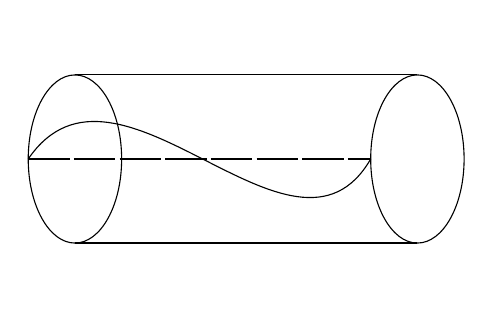
\begin{tikzpicture}[x=0.75pt,y=0.75pt,yscale=-1,xscale=1]
    %uncomment if require: \path (0,302); %set diagram left start at 0, and has height of 302

    %Shape: Ellipse [id:dp7113644287533367] 
    \draw   (220,160.5) .. controls (220,138.13) and (230.07,120) .. (242.5,120) .. controls (254.93,120) and (265,138.13) .. (265,160.5) .. controls (265,182.87) and (254.93,201) .. (242.5,201) .. controls (230.07,201) and (220,182.87) .. (220,160.5) -- cycle ;
    %Shape: Ellipse [id:dp2574876106229609] 
    \draw   (385,160.5) .. controls (385,138.13) and (395.07,120) .. (407.5,120) .. controls (419.93,120) and (430,138.13) .. (430,160.5) .. controls (430,182.87) and (419.93,201) .. (407.5,201) .. controls (395.07,201) and (385,182.87) .. (385,160.5) -- cycle ;
    %Straight Lines [id:da9747654267031158] 
    \draw    (242.5,120) -- (407.5,120) ;
    %Straight Lines [id:da6388065944921051] 
    \draw    (242.5,201) -- (407.5,201) ;
    %Straight Lines [id:da44727041223554886] 
    \draw  [dash pattern={on 15pt off 1.5pt}]  (220,160.5) -- (385,160.5) ;
    %Curve Lines [id:da44274218397801035] 
    \draw    (220,160.5) .. controls (263,97.5) and (348,224.5) .. (385,160.5) ;
  \end{tikzpicture}

  \caption{A standard section for $\check{X}([0,1])\simeq S^{1}\times [0,1]$}
\end{figure}

At first, we prove for projective tropical line $\mb{T}\mb{P}^{1}$.

\begin{proof}[Proof for tropical projective lines]

\end{proof}

\begin{Rmk}[Relations with sympletic geometry]
  In this paper, we usually assume every $C^{1}$-function has at most isolated critical point because we don't know about Morse-Bott functions for polyhedral complexes.
  $\check{X}_0([0,1])$ is a submanifold of a Liouville domain $[0,1]\times \R/\Z$ and
  the Liouville completion of $[0,1]\times \R^{\vee}/\Z^{\vee}$ is
  isomorphic to $\check{X}(\R)\simeq \R\times \R^{\vee}/\Z^{\vee}$.
  We can see such a Lagrangian section as
  a Lagrangian submanifold of the exact
  Lagrangian submanifold $\check{X}(\R)\simeq T^{*}S^{1}$
  such that the exact $1$-form vanishes on the complement
  of a compact set and invariant for the flow of
  the Liouville vector field
  \footnote{A \ind{Liouville vector field}{Liouville vector field}
    on a symplectic manifold $(M,\omega)$ is a vector field $V$ such that $L_V\omega =\omega$. If a Liouville vector field exists $V$ $i(V)\omega$ is a Liouville $1$-form and this transformation is bijective since $\omega$ is nondegenerate.}.
  associated with the tautological $1$-form on $T^{*}S^{1}$.
  Lagrangian submanifolds of this type have
  a central role of \ind{wrapped Fukaya category}{wrapped Fukaya category}.
  We will mention more about this in \cref{sec: toric}.
\end{Rmk}

\begin{Eg}
  Let $U$ be a sufficiently small open domain of an $n$-valent vertex $v$ of tropical curve.

  \begin{align}
    \opn{ind}_v(s_{p,q})=1-q, \quad
    \opn{ind}_v(-s_{p,q})=\opn{ind}_v(s_{q,p})=1-p.
  \end{align}

  when $n=p+q=3$,

  \begin{align}
    \opn{ind}_v(s_{3,0})=1, \quad \opn{ind}_v(s_{2,1})=0, \quad \opn{ind}_v(s_{1,2})=-1, \quad \opn{ind}_v(s_{0,3})=-2.
  \end{align}

\end{Eg}


\begin{DefProp}
  Let $B$ be a compact tropical curve and $s:B \to \check{X}_0(B)$ a continuous section of
  the surjection $\check{\pi}_{B}:\check{X}_0(B)\to B$
  such that $\check{\pi}_B(\opn{Im}s\cap \opn{Im}s_0)$ is discrete.

  The \ind{rotation number}{rotation number} of $s$ is the sum $\opn{rot}(s)\deq \sum_{e\in \pi_0(B_0)} \opn{rot}(s|_{\opn{cl}(e)})$ of rotation number
  of all closed edge whose interior is a connected component of $N$.
  \begin{align}
    \opn{rot}(s)=\opn{deg}(D_s)(=c_1(D_s))
  \end{align}

\end{DefProp}

\begin{proof}
  Compare the \v{C}ech cocycle between smooth Cartier data and ordinary Cartier data.
\end{proof}

\begin{Thm}[Pick's formula for tropical curve]
  Let $B$ be a compact tropical curve and $s:B \to \check{X}_0(B)$ a continuous section of
  the surjection $\check{\pi}_{B}:\check{X}_0(B)\to B$
  such that $\check{\pi}_B(\opn{Im}s\cap \opn{Im}s_0)$ is discrete.
  Then,
  \begin{align}
    \chi(B,s)=\opn{deg}(D_s)+1-g(B).
  \end{align}
  where $g(B)\deq \rank H^{1}(B,\Z)$.
\end{Thm}

\begin{proof}



  We can deform $s$ to a new section $s'$
  such that $\opn{ind}_v(s')=1$ for every vertex $v\in B\setminus B_0$.

  Under this deformation, the number $\chi(B,s)$ and $\opn{rot}(s)$ have no change.

  Choose a connected component $e$ of $B_0$.

  By replacing $s'|_{e}$ to the standard section, we get a new section $s_1$.

  The difference $\chi(B,s')-\chi(B,s_1)$ is equal to $\opn{rot}(s'|_{\opn{cl}(e)})$. By repeating this process, we can construct a new section $s_m$ such that every
  restriction of $s_m$ to a connected component of $B_0$ is a standard section.
  Obviously, $\opn{rot}(s_m)=0$, $\chi(B,s_m)= \sharp (B\setminus B_0) -\sharp \pi_0(B_0)=\chi_{\opn{top}}(B)$ and $\chi(B,s')-\chi(B,s_m)=\opn{rot}(s')$.

  In summary,
  \begin{align}
    \chi(B,s)=\opn{rot}(s)+\chi_{\opn{top}}(B)=\opn{deg}(D_s)+\chi_{\opn{top}}(B).
  \end{align}

\end{proof}

\begin{Rmk}
  We can naturally generalize this Pick's formula for "Lagrangian multi-section" of tropical curves.

  If $B$ is a tropical elliptic curve. This can be considered as a mirror of holomorphic vector bundle on the complex elliptic curve $X(B)$.

  This can be considered as the pushforward of line bundle by harmonic map.

\end{Rmk}

\begin{Rmk}
  If $D$ is BS type, then $\opn{deg}(D)+1-g\geq \sharp V(C)$ and thus
  $\opn{deg}(D)-\sharp V(C)\geq g-1$.
  From this we can easily see there exists an effective (resp. very ample) divisor $D$ such that
  $D$ is not BS type if $g\geq 2$.
  If $C$ is a trivalent metric graph, then every BS type divisor is very ample if $g\geq 4$ since
  $\sharp V(C)+g-1=3g-3$

  From the existence of winning strategy of chip-firing game \cite[Thereom 1.9]{MR2355607},
  every effective divisor has sufficiently large multiple $nD$ such that
  $nD$ is a Bohr-Sommerfeld type.



  From the philosophy of mirror symmetry, the desired associated cohomology is compatible with
  the rank of divisor on Mumford curves.
  See also \cite[Remark 2.9]{MR2448666} for an example of the specialization inequality is strict.
  (This remark is not in arXiv preprint.)
\end{Rmk}

\subsection{Proof for Hessian manifolds}


Let $f:X\to Y$ be a morphism of rational polyhedral space.
Then, this induces the pullback $f^{-1} $ and ring homomorphism
$f^{*}:H^{\bullet,\bullet}(Y)\to H^{\bullet,\bullet}(X)$ \cite[Proposition 4.17]{gross2019sheaftheoretic}. In particular, we have
$c_1(f^{*}(D))^{n}=f^{*}(c_1(D)^{n})$ for every $D\in\opn{Div}(Y)$.
\subsubsection{Verdier duality of rational polyhedral spaces}

Every rational polyhedral space $X$ is locally compact and $\Z$ is has finite homological dimension.

Thus, we can use Verdier duality of tropical spaces.
Recall the following elementary quasi-isomorphism.
\begin{align}
  \upomega_X=a_X^{!}\Z\simeq (a_Y\circ f)^{!}\Z \simeq f^{!}a_Y^{!}\Z=f^{!}\upomega_Y
\end{align}

The \ind{trace map}{trace map} of $X$ is the counit
$\int_X=\vep(X):Rf_!f^{!}\Z\to \Z$.

\begin{Prop}[Composition of ]
  \begin{align}
    (F\circ F')(G\circ G')(X)\to X
  \end{align}

  \begin{align}
    Rg_*Rf_*f^{!}g^{!}(\Z_X)\xto{\int_X\circ g^{!}}
  \end{align}

\end{Prop}

\subsubsection{Borel-Moore homology of rational polyhedral spaces}
The $(p,q)$-th Borel-Moore homology of $X$ is
\begin{align}
  H^{\opn{BM}}_{p,q}(X;\Z)\deq H^{-q}R\opn{Hom}(\Omega_X^{p},\upomega_X)
\end{align}

\begin{Eg} (i) $H_{0,q}^{\opn{BM}}(X;\Z)=H^{-q}R\opn{Hom}(A_X,\upomega_X)$ is equal to the classical Borel-Moore homology
  \cite[Lemma 4.8]{gross2019sheaftheoretic}.

  Since $B$ is a locally compact space,

  \begin{align}
    H_{0,0}^{\opn{BM}}(X;\Z)\simeq \Z,\quad H^{\opn{BM}}_{n,n}(X,\Z)\simeq \opn{Hom}_{\opn{D}(\Z_X)}(\upomega_X,\upomega_X)\simeq
    \opn{Hom}_{\opn{D}(\Z)}(R\Gamma_c\upomega_X,\Z)
  \end{align}

  (ii)

\end{Eg}



\begin{Prop}

  \begin{align}
    f^{\flat}:\Omega_Y^{*}\to f_*\Omega_X^{*}, \quad b_f: \Omega_Y^{*}\to f_*\Omega_X^{*} \to Rf_*\Omega_X^{*}
  \end{align}
  \begin{align}
    (g\circ f)^{\flat}=g_*(f^{\flat})\circ g^{\flat},
    \quad b_{g\circ f}=Rg_*(b_f)\circ b_g
  \end{align}
\end{Prop}
\begin{proof}

\end{proof}

\begin{Def}[{\cite[Definition 4.9]{gross2019sheaftheoretic}}]

  \begin{align}
    \opn{Hom}_{\opn{D}(\Z_X)}(\Omega_X^{p}[q],\upomega_X)\xto{Rf_*}
    \opn{Hom}_{\opn{D}(\Z_Y)}(Rf_*\Omega_X^{p}[q],Rf_*\upomega_X)
    \\
    \opn{Hom}_{\opn{D}(\Z_Y)}(Rf_*\Omega_X^{p}[q],Rf_*\upomega_X)
    \xto{\opn{Hom}(b_{f},Rf_*\upomega_X)}
    \opn{Hom}_{\opn{D}(\Z_Y)}(\Omega^{p}_Y[q],Rf_*\upomega_X) \\
    \opn{Hom}_{\opn{D}(\Z_Y)}(\Omega^{p}_Y[q],Rf_*\upomega_X)
    \xto{\opn{Hom}(\Omega_Y^{p}[q],\int_{X/Y})} \opn{Hom}_{\opn{D}(\Z_Y)}(\Omega_Y^{p}[q],\upomega_Y)
  \end{align}

  where

\end{Def}

\begin{align}
  \int_{X/Z}=\int_{Y/Z} \circ Rg_*\circ \int_{X/Y}
\end{align}

\begin{Prop}
  Let $f:X\to Y$, $Y\to Z$ be a proper morphism of rational polyhedral spaces
  In particular, $\int_X=\int_Y\circ f_*$.
\end{Prop}
\begin{proof}
  As mentioned in \cite[4.4]{gross2019sheaftheoretic}, this proposition comes from functoriality of derived pushforwards.
  We check about this.

  $f^{\flat}$

  \begin{align}
    \opn{Hom}(b_{g\circ f},R(g\circ f)_*\omega_X)
    =\opn{Hom}(b_g,R(g\circ f)_*\omega_X)\circ\opn{Hom}(Rg_*(b_f),R(g\circ f)_*\omega_X)
  \end{align}
  where
  \begin{align}
    \opn{Hom}(\Omega_{Z}^{p}[q],\int_{X/Z})=
    \opn{Hom}(\Omega_Z^{p}[q],\int_{Y/Z})\circ \opn{Hom}(\Omega_Z^{p}[q],Rg_*\circ \int_{X/Y})
  \end{align}

  \begin{align}
    \opn{Hom}(Rg_*(b_f),R(g\circ f)_*\upomega_X): &                                                                            \\
    \opn{Hom}_{\opn{D}(\Z_Z)}(R(g\circ f)_*\Omega_X^{p}[q],R(g\circ f)_*\upomega_X)
                                                  & \to \opn{Hom}_{\opn{D}(\Z_Z)}(Rg_*\Omega_Y^{p}[q],R(g\circ f)_*\upomega_X)
  \end{align}

  \begin{align}
    \opn{Hom}(b_g,R(g\circ f)_*\upomega_X): &                                                                        \\
    \opn{Hom}_{\opn{D}(\Z_Z)}(Rg_*\Omega_Y^{p}[q],R(g\circ f)_*\upomega_X)
                                            & \to \opn{Hom}_{\opn{D}(\Z_Z)}(\Omega_Z^{p}[q],R(g\circ f)_*\upomega_X)
  \end{align}

  Therefore,
  \begin{align}
    \opn{Hom}(Rg_*(b_f),R(g\circ f)_*\upomega_X)\circ Rg_*= Rg_*\circ \opn{Hom}(b_f,Rf_*\upomega_X)
  \end{align}

  \begin{align}
    \opn{Hom}(b_{g},R(g\circ f)_*\omega_X)\circ Rg_*:                           \\
    \opn{Hom}_{\opn{D}(\Z_Y)}(\Omega_Y^{p}[q],R f_*\upomega_X)
     & \to \opn{Hom}_{\opn{D}(\Z_Z)}(\Omega_Z^{p}[q],Rg_*(Rf_*f^{*}\upomega_Y))
  \end{align}

  \begin{align}
    \Omega_Z^{p}\to (g\circ f)_*\Omega_{X}^{p}\to R(g\circ f)_*\Omega_{X}^{p}
  \end{align}

  When $Z=\{\opn{pt}\}$, then $\upomega_Z=\Z_{\{\opn{pt}\}}$
\end{proof}

On the other hand,

$\frown: H^{p,q}(Y) \otimes H_{i,j}^{\opn{BM}}(Y)\to H_{p-i,q-j}^{\opn{BM}}(Y)$

$c\in H^{p,q}(Y)$
Let $f:X\to Y$ be a proper morphism of rational polyhedral spaces.
\begin{align}
  f_*(f^{*}c\frown \alpha)=c\frown f_*\alpha\in H_{p-i,q-j}^{\opn{BM}}(Y)
\end{align}
\begin{Eg}
  Consider the cap product
  $\frown:H^{n,n}(Y)\otimes H_{n,n}^{\opn{BM}}(Y)\to H^{\opn{BM}}_{0,0}(Y)$
  Recall, $H^{\opn{BM}}_{0,i}(Y;A)=H_{i}^{\opn{BM}}(Y;A)$ and$H_{0}^{\opn{BM}}(Y;\Z)$
  is isomorphic to $\Z$. This isomorphism is given from the following isomorphism.
  $H_{0}^{\opn{BM}}(X;A)\simeq
    \mb{H}^{0}(X;\upomega_X)\to \mb{H}_c^{0}(X;\upomega_X) \xto{\int_X} A$.
  On the other hand,

  $f_*:H_{n,n}^{\opn{BM}}(X)\to H_{n,n}^{\opn{BM}}(Y)$

\end{Eg}
\begin{Def}[degree of proper morphism]
  Let $f:X\to Y$ be a morphism of rational polyhedral spaces the pushforward
  $f_*:H_{n,n}^{\opn{BM}}(X)\to H_{n,n}^{\opn{BM}}(Y)$ $\int_X$

  the \ind{degree}{degree} of $f$.
\end{Def}


\subsubsection{Tropical cycle and cycle map}

Let $A$ be a tropical $k$-cycle.
\cite[Definition 3.6]{gross2019sheaftheoretic}
\begin{align}
  f_*A(y)=\sum_{x\in f^{-1}(y)}[T^{\Z}_yY:d_xf(T^{\Z}_x X)]A(x)
\end{align}

\begin{Def}

\end{Def}

For classical cases,

If $B$ is an integral affine manifold, then $B\setminus B_0=\emp$ and thus the Chern class of $B$ is trivial.



Therefore, $\opn{td}(B)$ should be $1$.

This proposition is an analog of \'{e}tale multiplicity of Euler characteristics
(cf. \cite[Proposition 1.1.28]{}).

\begin{Eg}[Frobenius splitting of tropical varieties]

  This is not a morphism of tropical space in the sense of
  \cite{gross2019sheaftheoretic} but this is a (local) morphism
  of monoidal spaces (e.g. \cite[II Definition 1.1.1]{MR3838359}).

\end{Eg}

\begin{Lem}

\end{Lem}

\begin{Lem}
  Let $f:B\to B'$ be a proper tropical morphism.
  \begin{align}
    \int_{B} f^{*}c\frown \alpha=\int_{B'} f_*(f^{*}c\frown \alpha)
    =\int_{B'}c \frown f_*\alpha=\opn{deg}(f)\int_{B'} c\frown \alpha
  \end{align}
\end{Lem}

\begin{proof}
  The right side follow from \cref{thm:}.
\end{proof}

\begin{Not}
  $\int_B$
\end{Not}

\begin{Thm}
  Let $B_0$ be a $n$-dimensional compact integral affine manifold and
  $s$ a smooth Lagrangian section
  whose intersection point are discrete.
  \begin{align}
    \chi(B_0,s)=\frac{1}{n!}\int_{B_0}c_1(D_s)^{n}.
  \end{align}

\end{Thm}
\begin{proof}

  If $B_0$ is a tropical tori, the statement of is true from \cite[]{} and \cref{eg: lattice tori}.

  From Cheng-Yau's result, $B_0$ is a finite unramified cover of tropical tori.
  Fix an \`etale cover $f:T \to B_0$ of $B_0$.

  Let $s$ be a Lagrangian section $s:B\to \check{X}(B_0)$.

  \begin{align}
    \chi(T,\tilde{s})=\opn{deg}(f)\chi(B_0,s),\quad \int_{T}(c_1(f^{*}(D_s))^{n})=\opn{deg}(f)\int_{B}c_1(D_s)^{n}
  \end{align}

  Combing this, we prove the formula.

\end{proof}




\section{tropical toric varieties} \label{sec: toric}

Tropical toric varieties are not main topics of this paper,
but we mention about them for revealing the relationship
between the theory of lattice polytopes in the sense of
toric varieties and our index.

See also \cite{coxToricVarieties2011a} for fundamental properties of classical toric varieties.


For simplicity, we fix $N=\Z^{n}$.

We recall about toric varieties over tropical semifield or semifield
from \cite{MR2428356} and potential .

We first recall the limit of polynomial over log-semiring $\underline{\R}_{\opn{log}}$
by Viro and Maslov's method.

Let $(\R_{\geq 0},0,1,+,\cdot)$ be the subsemifield
of nonnegative real numbers in $\R$ and we denote it by $\R_{\geq 0}$
for simplicity.
The logarithmic map
$T\log : \R_{\geq 0}\to \R\cup \{-\infty\}; x\mapsto T\log (x)$ where $T\log (0)=-\infty$
is a bijection and thus we can induce an addition $\oplus_{T}$
and a multiplication $\odot_{T}$ on $\underline{\R}$:
\begin{align}
  x\oplus_{T}y \deq T\log(\opn{exp}(\frac{x}{T})+\opn{exp}(\frac{y}{T})),
  \quad x\odot_T y \deq T\log(\opn{exp}(\frac{x}{T})\cdot\opn{exp}(\frac{y}{T}))=x+y.
\end{align}




$\underline{\R}_{\opn{log}}\deq \underline{\R}_{\opn{log},1}$ is called \ind{Log semiring}{Log semiring}.



From construction, $\underline{\R}_{\opn{log},T}$ is isomorphic to
$\R_{\geq 0}$ as a semifield and thus any algebra over
$\underline{\R}_{\opn{log},T}$ is equivalent to
an algebra over $\R_{\geq 0}$.

By taking a limit $T\to 0$, we get $x\oplus_T y\to \opn{max}\set{x,y}$
and thus $\underline{\R}_{\opn{log},T} \to \underline{\R}_{\max}$.



This operation can be generalized for measure space quickly and this is called Laplace principle

Besides, there exists the canonical isomorphism
$\mcal{O}_{B,\underline{\R}_{\max}}^{\times}
  \simeq \mcal{O}_{B,\underline{\R}_{\log}}^{\times}$
for sheaf of abelian groups.

Let $f:\R^{n}\to \R$ be a $\underline{\R}_{\opn{log}}$-valued
Laurent polynomial function on a splitting
$n$-torus over $\underline{\R}_{\opn{log}}$:

\newcommand{\biglogplus}{\bigoplus}

\begin{align}
  f(x) \deq \bigoplus_{m \in (\R^{n})^{\vee}} a_m\odot x^{\odot m}
  =\log (\sum_{m \in (\R^{n})^{\vee} }\opn{exp}(a_m+\abk{x,m})).
\end{align}

Every Laurent polynomial function is smooth and convex on $\R^{n}$
\footnote{$f(x,T)$ also convex on $\R^{n}\times \R_{>0}$}.

Therefore, $(\R^{n},f)$ forms an integral Hessian manifold.



Since $\R^{n}$ is an integral affine manifold, we can consider $1$-form $df$ as a smooth map
$df: \R^{n}\to \R$.

\begin{align}
  df(x)= \frac{1}{\sum_{m\in A} \opn{exp}(a_m)\cdot\opn{exp}(\abk{x,m})}
  \sum_{m\in A} \opn{exp}(a_m)\cdot\opn{exp}(\abk{x,m})m
\end{align}

The image of $1$-form $df:\R^{n}\to (\R^{n})^{\vee}$ is
homeomorphic to $\opn{relint}(\opn{Newt}(f))$ \cite[p.124 Exercise]{MR1301331}.

From properties of Hesse domains, $(\R^{n},Ddf)$ and
$(\opn{int}(\Delta^{[n]}),\check{D}d\check{f})$ are isometrics
Riemannian manifolds \cite[Proposition 2.3.3]{}.

As mentioned in the section of Hessian manifolds, the pullback of smooth convex function
is a K\"ahler potential function on $\check{X}(\R^{n})\simeq \R^{n} \times (\R^{n})^{\vee}/(\Z^{n})^{\vee}$
globally since $\R^{n}$ is simply connected.


\begin{align}
  \lim_{T\to +0} T \log \Paren{\int_X e^{\frac{f(x)}{T}}d\mu}=
  \opn{ess}\!.\!\sup_{x\in X}\{f(x)\}
\end{align}

\begin{align}
  \sqrt{-1} \partial \bar{\partial}
  \log(1+\sum_{i=1}^{n}\opn{exp}(2\log |z_i|))
  =\sqrt{-1} \partial \bar{\partial}\log(1+\sum_{i=1}^{n}|z_i|^{2})
\end{align}
This is the restriction of Fubini--Study metric on algebraic torus
$(\C^{\times})^{n}$ \cite[Examples 3.1.9 i)]{MR2093043}.
See also \cite[Appendix 2]{MR1301331} for general theory for
the relationships for Hessian form and the induced K\"{a}hler potential for
toric manifolds.

This is a tropical analog of weighted algebraic moment map.



\begin{Eg}[Moment map for tropical projective space]
  The dual Hessian
  $\check{f}:\opn{int}(\Delta^{[n]})\to \R;
    (x_1,\ldots,x_n)\mapsto
    \sum_{i=1}^{n}x_i\log x_i+(1-\sum_{i=1}^{n}x_i )\log (1-\sum_{i=1}^{n}x_i )$
  is the Shannon entropy of the sample space $\Omega=\set{0,\ldots,n}$.



  Therefore, the $n$-simplex can be considered as the discrete probability space of
  $\Omega$.

\end{Eg}

\begin{Eg}
  Since $\opn{exp}(x)=\opn{log}(e^{e^{x}})=$
\end{Eg}

gives a surjection $h:\Delta^{[m]}\to P$ induces
$S^{\oplus\Delta^{[m]}(\Z)}\to S^{\oplus P(\Z)}$ and the homogeneous
semiring
$\bigoplus_{n=0}^{\infty} S^{\oplus n\Delta^{[m]}(\Z)}
  \to \bigoplus_{n=0}^{\infty} S^{\oplus nP(\Z)}$ naturally.

This interpretation is important for algebraic statistics
and information geometry.

We can extend $df: \R^{n}\to (\R^{n})^{\vee}$ to

$df:X_{\Sigma(P)}^{\opn{trop}}\to (\R^{n})^{\vee}$ naturally and
$\opn{Im}(df)=\opn{Newt}(f)$.

Here, $\Sigma(P)$ is the normal fan of $P$.



$\mu_P^{\opn{trop}}$ is called the \ind{tropical moment map}{tropical moment map} of $(X_{\Sigma}^{\opn{trop}})$.

This is a tropical analog of algebraic moment map.

The phenomena of

\begin{Rmk}
  We expect that we can generalized for rational function
  over $\underline{\R}_{\opn{log}}$ and its differential is
  commutative with the moment map in the sense of .
\end{Rmk}

\begin{Lem}
  Let $f:C \to \R$ be a Morse function on a $2$-dimensional polyhedral cone $C$ with an isolated critical point at $0$.
\end{Lem}


The following Proposition is

\begin{Prop}[Ehrhart's reciprocity law revisit]
  Let $\mu_P: X_{\Sigma (P)}^{\opn{trop}}
    \to \check{X}_0(X_{\Sigma (P)}^{\opn{trop}})$
  be the tropical moment map of a lattice polytope $P$.
  \begin{align}
    \chi(X_{\Sigma(P)}^{\opn{trop}},\mu_P)=\sharp (P(\Z)),
    \quad \chi(X_{\Sigma(P)}^{\opn{trop}},-\mu_P)=(-1)^{n}\sharp (\opn{relint}(P)(\Z))
  \end{align}
\end{Prop}
\begin{proof}
  The associated local regular function over $\underline{\R}_{\opn{Log}}$ is minimum at the each vertex.
  Thus, this proposition is trivial.
\end{proof}
\begin{Def}

\end{Def}

\begin{Prop}
  $f:X_{\Sigma}^{\opn{trop}}\to \R$ be a $C^{1}$-function on $X_{\Sigma}^{\opn{trop}}$ and $[f]:X_{\Sigma}^{\opn{trop}} \to \check{X}_0(X_{\Sigma}^{\opn{trop}})$ the associated Lagrangian section.
  Then, $\chi(X_{\Sigma}^{\opn{trop}},[f])=1$.
\end{Prop}
\begin{proof}
  From Poincar\'e-Hopf theorem,
\end{proof}

\begin{Note}
  We didn't discuss for twisted polytope, i.e., a Cartier data of $T$-equivalent line bundle on $X_{\Sigma}$.
  Twisted polytope is deeply studied by \cite{MR1243782}.
  We develop about in future works but we mention a few comments about our expectation.
  Let $s:B_0 \to \check{X}(B_0)$ be a Lagrangian section of integral affine manifold.
  We already mention the expected differential $\mf{m}_1: \opn{CF}^{\bullet}(s)\to \opn{CF}^{\bullet}(s)$ is nonzero morphism in general case.

  If $\mf{m}_1$ is zero morphism, we can say $H^{p}(\opn{CF}^{\bullet}(s))=\opn{CF}^{p}(s)$.

  We expect that our graded complex is essentially
  equal to the decomposition of sheaf cohomology
  $\bigoplus_{m\in M}H^{p}(X_{\Sigma},\mcal{L})_m\simeq \opn{CF}^{p}(s)$ \cite[Theorem 9.1.3]{coxToricVarieties2011a}
  or \cite{MR1243782}.
  If this is true for every Cartier divisor on $X^{\opn{trop}}_{\Sigma}$,

\end{Note}



\subsection{Relationships between wrapped Fukaya category and localization of index}

Be careful of the standard isomorphism

\begin{align}
  (T^*N_{\R},\sum _idp_i\wedge dq_i)
  \simeq T^{*}M_{\R},-\sum_i dq_i\wedge dp_i),
  \quad (\check{X}(N_{\R}),\omega_{\opn{std}})\simeq (T^{*}(M_{\R}/M),-\omega_{\opn{std}}).
\end{align}

Let $\Lambda \subset T^{*}X$ be a conical Lagrangian subset

\begin{align}
  \Lambda_{\Sigma} =
  \bigcup_{\tau \in \Sigma}(\tau^{\bot} +M)\times -\tau,
  \quad \bar{\Lambda}_{\Sigma}\deq \opn{Im}(\pi:\Lambda_{\Sigma} \to T^{*}(M_{\R}/M))
\end{align}

\cite[Theorem 2, Corollary 2]{MR2871160}

\begin{align}
  \bar{\tau}:\mcal{P}\!\opn{erf}(X_{\Sigma})
  \to \opn{Fuk}(\check{X}(N_{\R});\bar{\Lambda}_{\Sigma}), \quad
  H^{0}(\bar{\tau}): \opn{D}^{b}(\opn{Coh}(X_{\Sigma}))\to
  \opn{D}(\opn{Fuk}(\check{X}(N_{\R});\bar{\Lambda}_{\Sigma})).
\end{align}


\footnote{This isomorphism is, however, for }

$\Phi_{}$

See also \cite[Appendix C.2.]{MR2871160} for relationships
between \cite{MR2871160} and \cite{MR2240909,MR2529936}.

Our tropical Lagrangian section for toric varieties is different from
that of \cite{MR2240909,MR2529936}.

In our definition of Lagrangian section and index, we do not define the higher operation
$\mf{m}_n$ so we only compare the objects.
In order to treat

\cite{MR3173401}
As the case of tropical curves, tropical toric varieties






\section{Preliminary of tropical manifolds}

\subsection{Definition of tropical spaces}
tropical piecewise linear spaces in the sense of \cite[Definition 2.1]{cavalieri2020tropical}
\footnote{We know the notion of tropical spaces
  in the sense of \cite[Definition 2.1]{cavalieri2020tropical} from the preprints by Yamamoto Yuto.}

\subsection{Definition of tropical manifolds}

We usually use max-plus algebra and thus we replace $\overline{\R}\deq \R \cup \{+\infty\}$ with $\underline{\R}\deq \R \cup\{-\infty\}$ from \cite{gross2019sheaftheoretic}.
There exists an exponential map $\opn{exp}: \underline{\R} \to \R_{\geq 0}$ and $\underline{\R}$ has the induced topology from the Euclidean topology of $\R_{\geq 0} (\subset \R)$. $\underline{\R}^{n}$ (resp. $\R^{n}$) is a tropical analogue of $n$-dimensional vector space $K^{n}$ (resp. split torus $(K^{\times})^{n}$) over a field $K$.

\begin{align}
  \R^{n}_{I}\deq \{(x_1,\ldots,x_n)\in \underline{\R}^{n} \mid x_i=-\infty \text{ if } i\in I \}\simeq \R^{n-\sharp I}
\end{align}

This strata gives the (tropical toric) stratification $\underline{\R}^{n}=\bigsqcup_{I\subset \{1,\ldots,r\}}\R^{n}_{I}$.
Let $\abk{\cdot ,\cdot}: (\R^{n})^{\vee}\times (\R^{n}) \to \R$ be the canonical linear pairing. A \ind{half space}{half space} in $\R^{n}$ is the set  $H_{m,a}\deq \{x\in \R^{n}\mid  \abk{m,x}\leq a\}$ for some $m\in (\R^{n})^{\vee}$ and $a\in \R$.
A \ind{convex polyhedron}{convex polyhedron} in $\R^{n}$ is a finite intersection of half spaces in $\R^{n}$.
$\R^{n}$ is the empty intersection of half spaces of $\R^{n}$.
From representation theorem for convex polyhedron (cf. \cite[Theorem 1.1,1.2]{MR1311028}), a convex polyhedron $P$ is bounded if and only if $P$ is a convex polytope.
A convex polyhedron is \ind{rational}{rational} if it is a finite intersection of $\{H_{m_i,a_i}\}_{i=1,\ldots,r}$ such that $m_i\in (\Z^{n})^{\vee}$ for all $i=1,\ldots,r$. A \ind{rational convex polyhedron}{rationalconvexpolyhedron} in $\underline{\R}^{n}$ is the closure of a rational convex polyhedron in $\R^{n}_I$ for some $I\subset \{1,\ldots,r\}$.


\begin{Def}
  A rational polyhedral space $(B,\mcal{O}_B^{\times})$ is a \ind{tropical space}{tropicalspace} if
\end{Def}


Let $\mcal{C}^{0}(B)$ be the sheaf of continuous $\R$-valued function on $B$ and $f:B\to B'$ be a continuous map. Then, there exists the pullback sheaf morphism $f^{\sharp}:f^{-1}\mcal{C}^{0}(B')\to \mcal{C}^{0}(B)$ such that $f^{\sharp}(U): C^{0}(f(U)) \to C^{0}(U);g \mapsto g\circ f $ for any open set $U$ in $B$. A morphism of rational polyhedral spaces is a continuous map $f:B\to B'$ such that
the pullback morphism $f^{\sharp}:f^{-1}\mcal{C}^{0}(B')\to \mcal{C}^{0}(B)$ induces a morphism $f^{-1}\mcal{O}^{\times}_{B'} \to \mcal{O}^{\times}_{B}$.

The natural morphism $\R_B \to \mcal{O}_{B}^{\times}$
induces the quotient sheaf \indse{\FBZ^{1}}{F1ZB}.
The sheaf $\mcal{F}^{1}_{\Z,B}$ is
called the \ind{cotangent sheaf}{cotangent sheaf} on $B$.
\indset{\FBZ^{0}}{\Z_{B}}{F0ZB}

\begin{align}
  \mathbf{F}_p^{\Z}(x)\deq
\end{align}

By taking total wedge product, we have a sheaf of graded ring
$\bigwedge^{\bullet} \FBZ^{1}$.
Let
$\iota:B^{\opn{reg}}\to B$ be the inclusion map.
$\iota_* ( \bigwedge^{\bullet} \FBZ^{1}|_{B^{\opn{reg}}})$

\subsection{Tropical superform}

The sheaf $\mcal{A}^{0,0}_B$ can be considered as the sheaf of
smooth functions on polyhedral space $B$.

Then, $\mcal{L}^{p}_{B}$ has the following acyclic resolution
and isomorphism \cite[Corollary 3.18, Lemma 3.21]{MR3903579}:
\begin{align}
  0 \to \mcal{L}^{p}_{B} \to \mcal{A}^{p,0}_{B}\xto{d''} \mcal{A}^{p,1}_{B} \xto{d''}\cdots ,\quad \mcal{L}^{p}_{B} \simeq \mcal{F}_B^{p}
\end{align}

Let $\mcal{Z}^{q}_{B}\deq
  \opn{Ker}(d'': \mcal{A}^{0,q}\to \mcal{A}^{0,q+1})$.





We need to mention
a functor $f^{!}$ is defined as a right adjoint to $Rf_!:\opn{D}^{}$
if $f_!$ has finite cohomological dimension
\cite[Theorem 3.1.5, Proposition 3.1.10]{}
\begin{align}
  R\opn{Hom}_{A_Y}(R f_!\mcal{F}^{\bullet},\mcal{G}^{\bullet})\simeq R\opn{Hom}_{A_X}(\mcal{F}^{\bullet},f^{!}\mcal{G}^{\bullet}) , \\
  \opn{Hom}_{\opn{D}^{+}(A_Y)}(Rf_! \mcal{F},\mcal{G})\simeq \opn{Hom}_{\opn{D}^{+}(A_X)}(\mcal{F},f^{!} \mcal{G})
\end{align}

Let $f:X\to Y$ be a continuous map between locally compact Hausdorff spaces

Let $\mcal{D}: \opn{D}(\Z_{B})\to \opn{D}(\Z_{B})$ be the Verdier dual functor.

$\upomega_X\deq a_X^{!}A_{\{\opn{pt}\}},\mcal{D}_{A_X}(\mcal{F}^{\bullet})\deq R\mcal{H}om_{A_X}(\mcal{F}^{\bullet},\mb{D}_{A_X})$

$\upomega_X$ is called the \ind{dualizing complex}{dualizingcomplex} over $A$ of $X$.

There exists the following quasi-isomorphism for a purely $n$-dimensional tropical manifold \cite[Theorem 6.2]{gross2019sheaftheoretic}.
\begin{align}
  \FBZ^{n-p}[n]\simeq \mcal{D}(\FBZ^{p})
\end{align}

We can discuss similar discussion which is used in applications of Verdier duality for Poincare duality as follows.
\begin{align}
  \opn{Hom}_{\opn{D}^{+}(\Z)}(R\Gamma_c(B,\Z_B),\Z)\simeq \opn{Hom}_{\opn{D}^{+}(\Z_{B})}(\Z_B, \FBZ^{n}[n] )\simeq \opn{Ext}^{n}(\Z_{B},\FBZ^{n})\simeq H^{n}(B,\FBZ^{n})
\end{align}
By taking shift functor, we have
\begin{align}
  \opn{Hom}_{\opn{D}^{+}(\Z)}(R\Gamma_c(B,\Z_B)[n-i],\Z)\simeq \opn{Hom}_{\opn{D}^{+}(\Z_{B})}(\Z_B, \FBZ^{n}[i] )\simeq \opn{Ext}^{i}(\Z_{B},\FBZ^{n})\simeq H^{i}(B,\FBZ^{n})
\end{align}
From universal coefficient theorem for PID-modules \cite[3.6.5]{MR1269324},
\begin{align}
  0 \to \opn{Ext}^{1}_{\Z}(H^{n-i+1}_c(B,\Z),\Z)\to H^{i}(B,\FBZ^{n}) \to H^{n-i}_c(B,\Z)^{\vee}\to 0
\end{align}





Since $B$ is a locally compact space, $H^{1}_c(B;\Z)$ is free (cf. \cite[VI. Proposition 5.3]{iversenCohomologySheaves1986a}) and thus $H_{0,0}^{\opn{BM}}(B;\Z)\simeq H^{n,n}(B;\Z)=H^{n}(B;\FBZ^{n})\simeq \Z$ if $B$ is compact and path-connected.
The associated map
$\opn{Hom}_{\opn{D}^{+}(\Z_{B})} (\mb{D}_B,\mb{D}_B)\simeq \opn{Hom}_{\opn{D}^{+}(\Z)}(R\Gamma_c\mb{D}_B,\Z)$
is called the \ind{trace map}{trace map} on $B$.

$f_*: H_{n,n}^{\opn{BM}}(X;\Z)\to H_{n,n}^{\opn{BM}}(Y;\Z)$ defines the degree of $f$.

$\mb{D}_X=a_X^{!}\Z\simeq (a_Y\circ f)^{!}\Z\simeq f^{!}a_Y^{!}\Z= f^{!}\mb{D}_Y$



\section{the case of tropical tori and integral affine manifolds}

\begin{Def}[integral affine manifold, Hessian manifold]

  An \ind{integral Hessian manifold}{integral Hessian manifold} is a pair of an integral affine manifold and Hessian form on it.

  

  \footnote{In many papers including \cite{kontsevichAffineStructuresNonArchimedean2006a} (resp. \cite{alexeevStablePairCompactification2019a}), tropical affine structure (resp. special tropical affine surface) is called integral affine structure (resp. integral-affine surface) or $\Z$-affine structure. In this paper differences between $(\opn{Aff}(M),M_{\R})$-structure and $(\opn{Aff}_{\R}(M),M_{\R})$-structure are significant, and thus we don't use this style.}

  \footnote{Hessian manifold is called
  \ind{K\"ahler affine manifold}{Kahler affine manifold}
  in \cite{MR714338}, \ind{affine K\"ahler manifold}{affine Kahler manifold}
  or AK-manifold for short.
  In the respect of history, we should use the latter name.
  However, we usually use the former name for avoiding the confusion
  of notion.}

\end{Def}

From now on we recall the commutative diagram (\ref{eq: smoothcartier})
 for integral affine manifolds.
and see additional properties for sheaves on integral affine manifolds.

From definition, there exists the isomorphism $\TBZ^{\vee}\simeq \mcal{F}_{\Z,B_0}^{1}$ and $\mcal{F}_{\Z,B_0}^{\bullet}\simeq \bigwedge^{\bullet}\TBZ^{\vee}$.


Of course, $\mcal{A}_{B_0}^{0,0}=\mcal{C}^{\infty}(B_0)$ and $\mcal{Z}^{1}_{B_0}$ is the sheaf of closed $1$-form on $B_0$.

We note this sheaf can be considered as the sheaf $\opn{Lag}(T^{*}B_0)$ of Lagrangian sections $s:U \to T^{*}U$ for open set $U \subset B_0$ , see some standard textbook for symplectic geometry such as \cite[3.2]{MR1853077}.

Another important thing is that $\mcal{Z}^{1}(B_0)/\mcal{T}_{\Z,B_0}^{\vee}$ (resp. $\mcal{C}^{\infty}(T^{*}B_0)/\mcal{T}_{\Z,B_0}^{\vee}$) is isomorphic to the sheaf of germs of Lagrangian sections (resp. smooth sections ) of the Lagrangian torus fibration $\check{f}_{B_0} :\check{X}(B_0)\to B_0$ \cite[(2.7), (2.11)]{duistermaatGlobalActionangleCoordinates1980a}.

Besides, $\mcal{C}^{\infty}(B_0)$ and $\mcal{C}^{\infty}(T^{*}B_0)$ are acyclic sheaves on $B_0$, the two map is surjective
\begin{align}
  H^{0}(B_0; \mcal{C}^{\infty}(B_0)/\AffS_{\Z,B_0})\xto{\delta_1} H^{1}(B_0;\AffS_{\Z,B_0}),\quad  H^{0}(B_0;\mcal{C}^{\infty}(T^{*}B_0)/\mcal{T}_{\Z,B_0}^{\vee})\xto{\delta_1}H^{1}(B_0;\TBZ^{\vee}).
\end{align}

$\bigwedge^{n}_{i=1}\TBZ\simeq \opn{or}(\Z_{B_0})$. Here $\opn{or}(\Z_{B_0})$ is the $\Z$-orientation sheaf on $B_0$.
If $A$ is a PID, there exists the following short exact sequence  by universal coefficient theorem:
\begin{align}
  0\to \opn{Ext}^{1}_{A}(H^{n-m+1}_c(B_0,A),A) \to H^{m}(B_0,\opn{or}^{A}_{B_0})\to H^{n-m}_c(B_0,A)^{\vee}\to 0
\end{align}
If
$B_0$ is $\Z$-orientable if and only if $B_0$ has a special integral affine structure. We note a connected manifold $B_0$ is $\Z$-orientable if and only if $H^{n}_c(B_0,\Z)\simeq \Z$
\cite[VI Theorem 6.4]{iversenCohomologySheaves1986a}.
Special integral affine manifold can be considered as a tropical analog of complex manifold with trivial Chern class and we will see this later.

\begin{align}
  \abk{\cdot,\cdot}: \bigwedge_{i=1}^{p} \TBZ\times  \bigwedge_{i=1}^{n-p} \TBZ \to \bigwedge_{i=1}^{n} \TBZ \simeq \opn{or}(\Z_{B_0}),\quad \bigwedge_{i=1}^{p}\TBZ^{\vee}\simeq \bigwedge_{i=1}^{n-p}\TBZ\otimes_{\Z_{B_0}}\opn{or}(\Z_{B_0})
\end{align}



\subsection{A crash course of SYZ mirror for tropical geometer}
In the previous section, we see that Lagrangian sections of integral affine manifold $B_0$ corresponds to section of $\mcal{M}^{\times}_{B_0}/\mcal{O}^{\times}_{B_0}$ which describe the Picard group $\opn{Pic}(B_0)$.
On the other hand, what is a good point of this correspondence for tropical geometry? One of important feature is that "Lagrangian sections have a good cohomology theory which corresponds to sheaf cohomology via Strominger-Yau-Zaslow's mirror symmetry." The cohomology is called \ind{Lagrangian Floer cohomology}{Lagrangian Floer cohomology} in symplectic geometry.
This strong point gives a Floer theoretic approach of "sheaf cohomology theory" for tropical geometry without discussing homological algebra over idempotent semiring 

Historically, integral affine manifolds are deeply-studied in the field of mirror symmetry as a toy model before the name of "tropical geometry" appear.

\ind{Strominger-Yau-Zaslow conjecture}{Strominger-Yau-Zaslow conjecture} or \ind{SYZ conjecture}{SYZ conjecture} is about a concrete method to solve Kontsevich's Homological Mirror Symmetry conjecture for Calabi-Yau manifolds.
\ind{Homological Mirror Symmetry}{Homological Mirror Symmetry} or \ind{HMS}{HMS} is a conjecture about categorical equivalence between two different triangulated category derived from symplectic geometry of Calabi-Yau manifold $\check{X}$ and complex geometry of a Calabi-Yau manifold $X$ (or a degenerate family of Calabi-Yau manifold $X_t$) \footnote{One of important motivation of HMS is a solution of \ind{Classical Mirror Symmetry}{classical mirror symmetry} which is appeared from string theory but we will not discuss about this since this solution is still an open question.}.

The triangulated category of symplectic geometric side come from a $A_{\infty}$-category which is called \ind{Fukaya category}{Fukaya category} of $\check{X}$.
An object of Fukaya category of $\check{X}$ is 
an oriented Lagrangian submanifold with additional data. 
The set of morphism is a graded vector space 
generated by a intersection point of two Lagrangian submanifolds 
when the two intersect transversely.

The  triangulated category of complex geometric side is the (bounded) \ind{derived category}{derived category} of coherent sheaves on $X$. This category is a powerful tool for the study of algebraic varieties and deeply studied.

Under assumption of SYZ conjecture, Lagrangian section of $s_{B_0}:B_0\to \check{X}(B_0)$ should map to a line bundle on $X(B_0)$. The goal of this subsection is about giving a reasoning about this, so symplectic geometers can skip this section. In this paper, Floer cohomology means that Lagrangian Floer cohomology.
\subsubsection{What is SYZ conjecture and HMS ?}

At first,

In order to explain SYZ conjecture and HMS, we need to prepare the notions of $A_{\infty}$-categories which need to define Fukaya category.
However, the notion of Fukaya category and $A_{\infty}$-category is too difficult, we only use a limited version of Fukaya category which is introduced in \cite[Chapter 8]{aspinwallDirichletBranesMirror2009} and we never discuss about the accurate definition and structure about Fukaya categories and $A_{\infty}$-categories.

\footnote{Surprisingly, the words 
"sheaf" or "sheaves" is only at page 13 in 
\cite{} and there is no such words in }

See \cite[Chapter1,2,3]{MR2244106} or \cite[4.4]{aspinwallDirichletBranesMirror2009} for fundamental properties of triangulated categories and derived category of coherent sheaves on algebraic variety.

\ind{Fukaya category}{fukaya category} is an $A_{\infty}$-category whose objects are Lagrangian submanifold with additional data.


Before recalling the definition of Fukaya category, we recall the statement about HMS and notions to state about it without explaining Fukaya category and the derived category of coherent sheaves on a variety.
Our explanation of Fukaya categories and $A_{\infty}$-categories
highly relies on \cite[Chapter 8]{aspinwallDirichletBranesMirror2009},
\cite[I]{MR2441780} and \cite{MR3848738}.


We assume every non-unital $A_{\infty}$-category is nonempty and $k$-linear.


$\opn{Fuk}(\check{X})$ is a \ind{cohomologically unital}
{cohomologically unital}, or \ind{c-unital}{c-unital},
i.e., $H^{\bullet}(\opn{Fuk}(\check{X}))$ is truly a category
\footnote{Usually, $A_{\infty}$-category means c-unital
  $A_{\infty}$-category like \cite[(2h) Terminology]{MR2441780}.}.
An non-unital $A_{\infty}$-functor is \ind{c-unital}{c-unital}
if $H^{\bullet}(f)$ is truly a functor of category.

A  c-unital $A_{\infty}$-functor $\Phi :\mcal{A}\to \mcal{B}$ is
\ind{quasi-equivalence}{quasi-equivalence} if the underlying
cohomological functor $H^{\bullet}(\Phi):H^{\bullet}(\mcal{A})
  \to H^{\bullet}(\mcal{B})$ is categorical equivalence
as graded linear categories.

In order to make $H^{0}(\opn{Fuk}(\check{X}))$ close to
$\opn{D}^{b}(\opn{Coh}(X))$, we need the following procedure.



For a given c-unital $A_{\infty}$-category $\mcal{A}$,
there exists a functorial way to define a new c-unital
$A_{\infty}$-categories $\opn{Tw}\mcal{A}$ which is called
the \ind{twisted $A_{\infty}$-category}{twisted Ainfty-category}.
Moreover, $\opn{Tw}\mcal{A}$ is a c-unital \ind{triangulated
  $A_{\infty}$-category}{triangulated Ainfty-category} of
$\mcal{A}$ \cite[Definition 8.15]{aspinwallDirichletBranesMirror2009}.
An another example of triangulated $A_{\infty}$-categories is
given from $\opn{D}^{b}(\opn{Coh}(X))$
\cite[8.2.1]{aspinwallDirichletBranesMirror2009},
which is denoted by $\opn{D}^{b}_{\infty}(\opn{Coh}(X))$.
This is a dg-enhancement of $\opn{D}^{b}(\opn{Coh}(X))$.

By \cite[Proposition 3.14]{MR2441780}, if $\mcal{A}$ is
a c-unital triangulated $A_{\infty}$-category
$H^{0}(\mcal{A})$ is a triangulated category and a c-unital
$A_{\infty}$-functor $\Phi:\mcal{A}\to \mcal{B}$ between
triangulated $A_{\infty}$-category induces an exact functor
$H^{0}(\Phi): H^{0}(\mcal{A})\to H^{0}(\mcal{B})$.

By \cite[Lemma 3.24, 3.25]{MR2441780},
every quasi-equivalent c-unital $A_{\infty}$-functor $\Phi:\mcal{A}\to \mcal{B}$ induces a new quasi-equivalent c-unital $A_{\infty}$-functor $\opn{Tw}(\Phi):\opn{Tw}(\mcal{A}) \to \opn{Tw}(\mcal{B})$.

A \ind{split-closure}{split-closure}

By \cite[Lemma 4.7,4.8]{MR2441780}, every c-unital $A_{\infty}$-category $\mcal{A}$ has a unique split-closure $(\mcal{B} ,\Phi:\mcal{A} \to \mcal{B}))$ up to quasi-equivalence and $\mcal{B}$ is a c-unital triangulated $A_{\infty}$-category when $\mcal{A}$ is a c-unital triangulated $A_{\infty}$-category.
The \ind{Karoubi completion}{Karoubi completion} is a typical split closure.

Let $\opn{D}^{\pi}_{\infty}(\opn{Fuk}(\check{X}))$ be the Karoubi completion of $\opn{Tw}(\opn{Fuk}(\check{X}))$ and $\opn{D}^{\pi}(\opn{Fuk}(\check{X}))\deq H^{0}(\opn{D}^{\pi}_{\infty}(\opn{Fuk}(\check{X})))$.

From the above process, we can state homological mirror symmetry conjecture as follows.
\begin{Conj}[Homological Mirror Symmetry(HMS)]
  Let $\check{X}$ be a Calabi-Yau manifold. Then, there exists a Calabi-Yau manifold $X$  which satisfies the following quasi-equivalence of $A_{\infty}$-categories and equivalence of triangulated categories: \footnote{However, the statement is not accurate enough and we mention about some points about it later.}
  \begin{align}
    \opn{D}^{\pi}_{\infty}(\opn{Fuk}(\check{X}))\simeq \opn{D}^{b}_{\infty}(\opn{Coh}(X)),\quad \opn{D}^{\pi}(\opn{Fuk}(\check{X}))\simeq \opn{D}^{b}(\opn{Coh}(X))
  \end{align}
\end{Conj}

The right side equivalence of triangulated categories follows from the left side quasi-equivalence.

Let's check the quick consequence of HMS. Let $\Phi: \opn{D}^{\pi}_{\infty}(\opn{Fuk}(\check{X}))\simto \opn{D}^{b}_{\infty}(\opn{Coh}(X))$ be a quasi-equivalent c-unital $A^{\infty}$-functor. Since $H^{i}(\opn{Hom}_{\opn{D}^{b}_{\infty}(\opn{Coh}(X))}^{\bullet}(\mcal{F}^{\bullet},\mcal{G}^{\bullet}))\simeq \opn{Ext}^{i}_{\mcal{O}_X}(\mcal{F}^{\bullet},\mcal{G}^{\bullet})$ \cite[8.2.1]{aspinwallDirichletBranesMirror2009}, we have the following isomorphism as graded vector spaces:
\begin{align}
  \opn{HF}^{\bullet}(\mathscr{L},\mathscr{L}')\deq H^{\bullet}(\opn{CF}^{\bullet}(\mathscr{L},\mathscr{L}'))\simeq \opn{Ext}^{\bullet}_{\mcal{O}_X}(\Phi(\mathscr{L}),\Phi(\mathscr{L}')).
\end{align}



In particular, the equivalence of small triangulated categories
$\mcal{D}\simeq \mcal{D}'$ induces a group isomorphism of
the Grothendieck group $\opn{K}(\mcal{D})\simeq \opn{K}(\mcal{D}')$
of triangulated categories.
Therefore, $\opn{K}(\opn{D}^{\pi}(\opn{Fuk}(\check{X})))\simeq \opn{K}(\opn{Coh}(X))$, see \cite[Exercise I.27]{}.

From construction, there exists a standard c-unital $A_{\infty}$-functor $\opn{Fuk}(\check{X})\hookto \opn{D}^{\pi}_{\infty}(\opn{Fuk}(\check{X}))$ and the underlying cohomological functor $H^{0}(\opn{Fuk}(\check{X})) \hookto \opn{D}^{\pi}(\opn{Fuk}(\check{X}))$.
Therefore, every object $\mathscr{L}$ of $\opn{Fuk}(\check{X})$
maps to a cochain complex of coherent sheaves $\mcal{F}^{\bullet}$
on $X$ and the Floer cohomology
$\opn{HF}^{\bullet}(\mathscr{L},\mathscr{L}')$
maps to Ext group
$\opn{Ext}^{\bullet}_{\mcal{O}_X}(\mcal{F}^{\bullet},
  \mcal{G}^{\bullet})$ of coherent sheaves.
In particular, if $\mathscr{L}_0$ is an object of
$\opn{Fuk}(\check{X})$ such that $\Phi(\mathscr{L}_0)
  \simeq \mcal{O}_X$ then
$\opn{HF}^{\bullet}(\mathscr{L}_0,\mathscr{L})\simeq
  \opn{Ext}^{\bullet}_{\mcal{O}_X}(\mcal{O}_X,\Phi(\mathscr{L}))\simeq
  \mb{H}^{\bullet}(X;\Phi(\mathscr{L}))$.



Strominger-Yau-Zaslow Conjecture is about a concrete method to create a c-unital $A_{\infty}$-functor $\Phi_{\opn{SYZ}}: \opn{Fuk}(\check{X})\to \opn{D}^{b}_{\infty}(\opn{Coh}(X))$ which induces a quasi-equivalence $\opn{D}^{\pi}_{\infty}(\opn{Fuk}(\check{X}))\simeq \opn{D}^{b}_{\infty}(\opn{Coh}(X))$.
\cite{stromingerMirrorSymmetryTduality1996}

\begin{Conj}[limiting version of Strominger-Yau-Zaslow(SYZ)]

\end{Conj}
If $\Phi_{\opn{SYZ}}: \opn{Fuk}(\check{X})\to \opn{D}^{b}_{\infty}(\opn{Coh}(X))$ exists, then $H^{0}(\Phi): H^{0}(\opn{Fuk}(\check{X}))\to \opn{D}^{b}(\opn{Coh}(X))$
describe the image of $\opn{Ob}(\opn{Fuk}(\check{X}))$ completely since $\opn{Ob}(H^{0}(\opn{Fuk}(\check{X})))=\opn{Ob}(\opn{Fuk}(\check{X}))$.

From now, we recall about objects of $\opn{Fuk}(\check{X})$ and morphisms.

Let's estimate what coherent sheaves correspond to Lagrangian sections via mirror symmetry.

The following explanation almost rely on \cite{MR3848738}.

There exists the following fully faithful exact functor
$\opn{D}^{b}(\opn{Coh}(X))\to \opn{D}^{b}(\opn{Qcoh}(X))\to \opn{D}^{b}(\mcal{O}_X\opn{-Mod})$ for Noetherian scheme $X$ over $k$.
In  general, $\opn{Coh}(X)$ does not has enough injectives
but $\opn{Qcoh}(X)$ has when $X$ is a Noetherian scheme.
Therefore, let $\mcal{F}^{\bullet},\mcal{G}^{\bullet}\in \opn{Ob}(\opn{D}^{b}(\opn{Coh}(X)))$ be coherent sheaves on $X$ then $\opn{Ext}^{i}_{\mcal{O}_X}(\mcal{F}^{\bullet},\mcal{G}^{\bullet})\simeq \opn{Hom}_{\opn{D}^{b}(\opn{Coh}(X))}(\mcal{F}^{\bullet},\mcal{G}^{\bullet}[i])$
\cite[Remark 2.57, 3.7]{MR2244106}.


To see objects in triangulated categories $\mcal{D}$, a \ind{spanning class}{spanning class} is useful \cite[Definition 1.47]{MR2244106}. When $\mcal{D}=\opn{D}^{b}(\opn{Coh}(X))$, the family $\{k_{p}\}$ of skyscraper sheaves on closed points is a typical spanning class \cite[Proposition 3.17]{MR2244106}.
Since $\opn{Ext}^{\bullet}(k_{p},k_p)\simeq \bigwedge^{\bullet}k^{n}$,
$\opn{}(L,\mcal{L},\nabla)$

We need not discuss angle function and

From now, $B_0$ is a compact \ind{special integral affine manifold}{special integral affine manifold}, i.e., a compact integral affine manifold such that whose transition maps are in $\opn{SL}_n(\Z)\ltimes \R^{n}$. $B_0$ and Lagrangian section have a canonical orientation induced from special integral affine structure.


We explain Semi-flat SYZ transformation of Lagrangian sections.

At first,

If $s:B_0 \to \check{X}(B_0)$ is the zero section, the corresponding $U(1)$-connection on $X(B_0)$ should be flat,i.e., $\Phi_{\opn{SYZ}}(L_0)\simeq \mcal{O}_{X(B_0)}$



From now, we assume $\check{X}$ is a Calabi-Yau manifold on symplectic side and $X$ is a Calabi-Yau manifold on complex manifold side. Here $\Lambda_{\opn{nov}}$ is the \ind{Novikov ring}{Novikov ring} of integer and $\Lambda_{\opn{nov}}^{\mb{K}}\deq \Lambda_{\opn{nov}}\otimes_{\Z}\mb{K}$

\begin{align}
  \opn{CF}^{i}((L_1,\mcal{L}_1,\nabla),(L_2,\mcal{L}_2,\nabla))\deq \bigoplus_{x\in L_0\cap L_1,\opn{maslov}(x)=i} \opn{Hom}(\mcal{L}_1|_{p},\mcal{L}_2|_{p}) \otimes_{\mb{K}}\Lambda_{\opn{nov}}^{\mb{K}},
\end{align}

$\opn{HF}^{\bullet}((L_1,\mcal{L}_1,\nabla),(L_2,\mcal{L}_2,\nabla))\deq \opn{Ker}\mf{m}_1/\opn{Im}\mf{m}_1$

\begin{align}
  \opn{HF}^{\bullet}(L_1,\phi(L_1);\Lambda_{\opn{nov}}^{\C})\simeq H^{\bullet}(L_1,\Lambda_{\opn{nov}}^{\C}) , \quad \chi_{\opn{top}}(L_1)=\sum_{x\in L_0\cap L_1, \opn{maslov}(x)=i} (-1)^{i}
\end{align}

\begin{align}
  \opn{HF}^{\bullet}((L_1,\mcal{L}_1,\nabla),(L_2,\mcal{L}_2,\nabla)) \xto{\Phi_{\opn{SYZ}}} \opn{Ext}^{\bullet}(\Phi_{\opn{SYZ}}(L_1,\mcal{L}_1,\nabla) , \Phi_{\opn{SYZ}}(L_2,\mcal{L}_2,\nabla))
\end{align}





\begin{Eg}
  We can see the condition $[\omega]\cdot\pi_2(M,L)=0$ is strict from the following example.
  Let $B_0=\R/\Z$ and
  $\check{X}=\check{X}(B_0)$. Every submanifold of 2-dimensional symplectic manifold is Lagrangian. Take a small smooth closed disk $D$ at a fixed point. Then, the boundary $\partial D$ does not satisfy the above condition since the integral $\int_{D}\omega$ is obviously nonzero.

  On the other hand, every Lagrangian section $L_s$ of $B_0$ satisfies the condition because $\pi_{1}(B_0,p)\xto{s_*} \pi_{1}(\check{X},s(p))\xto{\check{\pi}_{B_0,*}}\pi_{1}(B_0,p)$ is the identity morphism, i.e., $\pi_1(L_s)\to \pi_1(\check{X})$ is injective and thus $\pi_2(\check{X},L_s)$ is trivial from exact sequence of relative homotopy group and the triviality of higher homotopy group of real tori except fundamental group.
  Therefore, $\opn{HF}^{\bullet}(L_s,L_s)\simeq H^{\bullet}(L_s,\Lambda_{\opn{nov}}^{\mathbb{K}})$. We can quickly generalize this when $\pi_2(\check{X}(B_0))\simeq \pi_2(B_0)$ is trivial.
  Every compact integral affine manifold with a Hessian form such that $\pi_2(B_0)$ is trivial since such manifold is a finite quotient of tropical tori by Cheng-Yau's result.
  \footnote{There exists a compact affine manifold $B_0$ such that $\pi_2(B_0)=\Z$ as explained in \href{https://mathoverflow.net/questions/271499/smooth-manifold-with-affine-structure-aspherical}{dg.differential geometry - Smooth manifold with affine structure: aspherical? - MathOverflow}. This affine manifold is called 3-dimensional \ind{affine Hopf manifold}{affine Hopf manifold}. A $n$-dimensional affine Hopf manifold is homeomorphic to $S^{1}\times S^{n-1}$. However, every affine Hopf manifold is not integral affine and has no Hessian form \cite[Corollary 7.3.5]{MR2293045}.}
  Markus's conjecture claim that every closed special affine manifold is complete and thus
  $\pi_2(B_0)=0$ follows if Markus's Conjecture is true.
  If $\pi_2(B_0)=0$, then $\pi_2(\check{X}(B_0),\check{f}^{-1}(b))=0$ for every torus fiber $\check{f}^{-1}(b)$  \cite[Theorem 4.41, Proposition 4.48]{hatcherAlgebraicTopology2002a}.
  Therefore,  \cite{MR4301560}.
\end{Eg}


\footnote{In some literature, the symbols $\check{X}(B_0)$ and $X(B_0)$ are opposite.}

Consider the self-intersection number of zero section $[L_0]\cap [L_0] \in H_{0}(\check{X}(B_0),\Z)$

$g(\opn{grad}f,X)=df(X)$, i.e., the gradient is defined from musical isomorphism.

\begin{Eg}[Generalized Pick's formula for line bundles on tropical tori] \label{eg: lattice tori}
  We add some comments about the previous remark in the case of tropical tori.
  First, we consider tropical version.
  Let $B_0=M_{\R}/\Lambda$ be a tropical torus and $\mcal{L}$ be a tropical line bundle on $B_0$. As explained in \ref{}, a Cartier data of $\mcal{L}$ can be described by a quadratic potential function $q$ on $M_{\R}$ up to affine functions and every Cartier divisor on integral affine manifolds can be considered as a Lagrangian section $s: B_0 \to \check{X}(B_0)$ which is induced from the 1-form $dq$ by the equation \ref{eq: }. For simplicity, we assume $c_1(\mcal{L})$ is a nondegenerate matrix. Then $q$ is a Morse function and $L_0 \cap L_s$ is a finite set. Thus, every Morse index at $x\in  L_0\cap L_s$ is equal to the index of $q$. In summary, we have
  \begin{align}
    [L_0]\cap [L_s]=\det (c_1(\mcal{L}))=\frac{c_1(\mcal{L})^{n}}{n!}.
  \end{align}
  When $c_1(\mcal{L})$ is a degenerate matrix, we can add a good periodic smooth function $h$ on $B_0$ such that $q+h$ is a Morse function and consider the Lagrangian section which is induced from the 1-form $d(q+h)$. Then, we also get the above formula for this cases, i.e., $[L_0]\cap [L_s]=0$.

  From now, we consider the mirror version. Let $D\in H^{1}(B,\TBZ)$

\end{Eg}

\begin{Eg}[{$\C$-local system on $L$ should be trivial in the tropical world}]
  The following analogue suggests that we only consider a certain analogue of classical Lagrangian Floer cohomology when we attack Riemann-Roch type theorem. Be careful this observation is false when we apply to Fukaya category for Calabi-Yau varieties.

  Let $B=\R/r\Z$ be a tropical elliptic curve

\end{Eg}

\subsubsection{More about mirror symmetry}

We only see the Mirror symmetry for Lagrangian torus fibration
with no singular locus.
We note about the work of 
\cite{grossSpecialLagrangianFibrations1998a,grossSpecialLagrangianFibrations1999}.



The ring structure of the total complex $E_2^{\bullet,*}=H^{\bullet}(B;R^{*}f_*\Z_X)$
is equal to the ring structure which is induced from 
$\mb{H}^{\bullet}(B;\bigoplus_{q\in \Z}R^{q}f_*\Z_X[-q])$. This ring structure induces
the cup product on $E_{r\geq 3}$-pages and $E_{\infty}$-pages.
These cup products compatible with those of 
 and $H^{\bullet}(X;\Z_X)$. (See \cite[IV 6.8., Appendix A]{bredonSheafTheory1997a}.)

If $\check{f}$ is $\Z$-simple \cite[Definition 2.1]{grossSpecialLagrangianFibrations1998a} 
, i.e., $\iota_*R^{q}\check{f}|_{f^{-1}(B_0),*}\Z_{\check{X}}\simeq R^{q}f_*\Z_{\check{X}}$.
then the pairing $R^{q}f_0\Z_{\check{X}} \times R^{n-q}f_0\Z_{\check{X}}\to \Z_{\check{X}}$
is perfect and thus
\begin{align}
R^{q}f_*\Z_X\simeq R^{n-q}\check{f}_*\Z_{\check{X}},
\quad H^{p}(B;R^{q}f_*\Z_X)\simeq H^{p}(B;R^{n-q}\check{f}_*\Z_{\check{X}}).
\end{align}

From the seven-term exact sequences of the Leray spectral sequence and \cite[Remark ]{}, 

Let $s:B\to \check{X}$ be a $C^{\infty}$-section, 

If $\check{X}$ is a simply connected Calabi-Yau threefold then the Leray 
spectral sequence degenerate at the $E_2$-term \cite[Theorem 3.9]{}.

\begin{Conj}[{Mirror Riemann-Roch \cite[Conjecture 4.9]{grossSpecialLagrangianFibrations1998a}}]
Let $(\check{X} \xto{\check{f}} B \xgets{f} X)$ be a $\Z$-simple SYZ pair in the sense of 
\cite[Definition 2.1, 2.3]{grossSpecialLagrangianFibrations1998a}.
\footnote{Please be careful that $\check{X}$ is a complex side in 
\cite{grossSpecialLagrangianFibrations1998a}.}
Let $D$ be a divisor class such that
$c_1(D)\in\opn{Ker}(H^{2}(X;\Z)\to H^{0}(B;R^{2}f_*\Z_{X}))$.
$[D]$ be a divisor
$L_{D}$ be a section of $f:X\to B$ which is defined

\begin{align}
    (-1)^{n(n-1)/2}[L_0] \cap [L_D]=\chi(\check{X},\mcal{O}(D))
  \end{align}
\end{Conj}

Take care the signature $(-1)^{n(n-1)/2}$. In fact, we can easily check $[L_0]\cap [L_0]=-2$ if $\check{X}\to B$ is a special Lagrangian torus fibration of K3 surfaces under hyperk\"ahler rotation from adjunction formula.

\subsection{Radiance obstruction and geometric prequantization}
In this subsection, we recall the relationships lattice points of strongly integral affine manifolds and geometric quantization from \cite{1999math......2027T,MR3112817,MR3525095}. A symplectic manifold $(M,\omega)$ is \ind{prequantizable}{prequantizable} if the de Rham cohomology class $[\omega]$ of $\omega$ is in $H^2(X,\Z)$. An integral affine manifold $B_0$ has a strongly integral affine structure if and only if the de Rham cohomology class of $\omega_{\opn{std}}(\in \check{X}(B_0))$ is in $H^{2}(\check{X}(B_0),\Z)$, see



From the theory of connection on a vector bundle,
 there exists a complex line bundle $\mcal{L}$ with a $U(1)$-connection $\nabla$ and $R_{\nabla}=-2\pi\sqrt{-1}\omega$.  Such pair $(\mcal{L},\nabla)$ is called \ind{prequantum line bundle}{prequantum line bundle} over $M$. Obviously, $c_1(\mcal{L})=[\omega]$.
Let $L$ be a Lagrangian submanifold of $(M,\omega)$.
Then, $\nabla|_{L}$ is a flat $U(1)$-connection from definition.
$L$ is a \ind{Bohr--Sommerfeld orbit}{bohr-sommerfeld orbit} if $\nabla|_{L}$ is a trivial connection on $L$. Let $\pi :M\to B$ be a Lagrangian fibration. A point $x\in B$ is \ind{Bohr--Sommerfeld point}{bohr-sommerfeld point} if $\pi^{-1}(x)$ is a Bohr-Sommerfeld orbit.

\begin{Eg}
The origin of Bohr-Sommerfeld orbit is from Old Quantum Theory.

Consider the Hamiltonian of $1$-dimensional harmonic oscillator;
  \begin{align}
    H(q,p)\deq \frac{p^{2}}{2m}+\frac{k}{2}q^{2},\quad  (m, k>0).
  \end{align}
Here, $m$ means the mass of harmonic oscillator and $k$ be a force constant.
  Let $X=\R^{2}$, $X_0= \R^{2}\setminus \{(0,0)\}$, $B=\R_{\geq 0}$ and $B_0=\R_{>0}$.

  In this case, $H^{2}(X_0,\Z)=H^{2}(X_0,\R)=0$ and thus $\omega/\hbar$ is quantizable for every $\hbar >0$.


  This is a typical example of $1$-dimensional mechanics.
  Each fiber $H^{-1}(E)$ is an ellipse except $E=0$. And thus $H: X_0\to B_0$ is a Lagrangian torus fibration. Let $\mcal{L}=X_0\times \C$ be a complex trivial line bundle.

  There exists $\nabla_X= (X-\frac{2\pi \sqrt{-1}}{\hbar}\theta(X))$, i.e., $\nabla =d-\frac{2\pi \sqrt{-1}}{\hbar}\theta$ and .

  \begin{align}
    R_{\nabla}(X,Y)=\nabla_X \nabla_Y-\nabla_{Y}\nabla_{X}-\nabla_{[X,Y]}=-2\pi \sqrt{-1}\omega(X,Y)/\hbar
  \end{align}

  Choose a parameter curve $x:[0,1]\to H^{-1}(E)$ and a local section $s$ which is parallel to $\dot{x}(t)$.

  The associated holonomy $e^{2\pi \sqrt{-1}\int_{H^{-1}(E)}\frac{1}{\hbar}pdq}$  is trivial if and only if $\frac{1}{ \hbar}\int_{H^{-1}(E)}pdq$ is an integer.

  This condition is compatible with \ind{de Broglie hypothesis}{de Broglie hypothesis} since the parallel transport can be considered as a wave function of a particle.
  See \cite[15.2, Chapter 22]{MR3112817} for more details about the above example.

  $\mcal{Q}_{\opn{pre}}(H)$ \cite[Proposition 22.6]{MR3112817}




\end{Eg}


Let $\check{f}_{B_0}:\check{X}(B_0)\to B_0$ be the standard Lagrangian torus fibration of a compact strongly integral affine manifold. By checking the holonomy representation of each cycle of fiber $\check{f}_{B_0}^{-1}(b)$,
the set of Bohr-Sommerfeld point of it is equal to $B_0(\Z)$.



The equation $\sharp (B_0(\Z))=\chi(\mcal{L},\nabla)=\opn{vol}(\check{X}(B_0))=\opn{vol}(B_0)$ can be computed by Atiyah-Singer's index formula \cite[Corollary 4.1]{MR1461965}.

(ii) We can see  $B_0(\Z)=f_{B_0}(s_{B_0} \cap s_0)$.

From the Morse index of potential multifunction at $x\in f_{B_0}(s_{B_0}\cap s_0)$, the signature index of every Bohr-Sommerfeld point is positive.

See
\href{https://arxiv.org/abs/1808.07305}{[1808.07305] Geometric quantization via SYZ transforms} for recent results on geometric quantization.



\subsection{Combinatorial Floer graded vector space and micro-localization}

\begin{Eg}[{\cite[p.22]{MR2031639}}]



\end{Eg}





\section{General setting}



\begin{Def}

  \begin{align}
    \chi(B,s)\deq \sum_{p\in \opn{Im} s_1 \cap \opn{Im} 0_B} \opn{Ind}(s_1,p), \quad   \chi(B,s_1,s_2)\deq \chi(B,s_2-s_1)
  \end{align}

\end{Def}

\begin{Rmk}
  Let $B$ be a compact integral affine manifold.
  \begin{align}
    \chi(B,s_1,s_2) & =\opn{deg}([\opn{Im}s_1]\cap [\opn{Im}s_2]) \\
    \chi(B,s_1,s_2) & =(-1)^{n}\chi(B,s_2,s_1)
  \end{align}
  Of course, the last equation is false in general compact tropical manifolds. This is an analog of Serre duality of algebraic varieties such that canonical divisor $\mcal{K}_X$ is trivial.

  \begin{align}
    \chi(\opn{Ext}^{\bullet}_{\mcal{O}_X}(\mcal{L}_2,\mcal{L}_1))=\chi(X,\mcal{L}_1\otimes \mcal{L}_2^{-1})= & (-1)^{n}\chi(X,\mcal{L}_1^{-1}\otimes \mcal{L}_2\otimes \mcal{K}_X)                     \\
    =                                                                                                        & (-1)^{n}\chi(\opn{Ext}^{\bullet}_{\mcal{O}_X}(\mcal{L}_1,\mcal{L}_2\otimes \mcal{K}_X))
  \end{align}

  \begin{Ques}
    \begin{align}
      \chi(B,s_2,s_1)=(-1)^{n}\chi(B,s_1,s_2+s_{K_B}) \quad ?
    \end{align}
  \end{Ques}

\end{Rmk}

\subsection{Future works}

\subsubsection{Sheaf theoretic version of this thesis}

From

From the success of the theory of tropical cohomology
$\mb{H}^{\bullet}(X;\mcal{F}_X^{\bullet})$,
we may expect that the category of constructible sheaf
on tropical geometry gives an analogue of coherent
sheaves on algebraic varieties.
There exist, however, evidences that
this expectation is not true.
Let $B$ an compact integral affine manifold and
$\opn{D}_c(B)$ be the sheaves of constructible sheaf
on
For sheaves $\mcal{F},\mcal{G}\in \opn{D}_{c}^{b}(B)$

$\chi(\mcal{F}\otimes_k \mcal{G})_x
  =\chi(\mcal{F})\cdot \chi(\mcal{G})_x$ for any point
$x\in B$.
\cite[(9.7.2)]{MR1299726}.
Therefore, a numerical function
$n\mapsto \chi(\mcal{F}^{\otimes n})=\chi(\mcal{F})^{n}$
is a sum of exponential functions and constant function.
Obviously, this properties is very far
from line bundles on algebraic variety for many cases.
For instance, $\omega_X$ is

From this properties, we need to consider different category
for

\begin{Eg}[An analog of Kodaira vanishing theorem]

  We don't define the differential
  $\mf{m}_1:\opn{CF}^{\bullet}(s,R)\to \opn{CF}^{\bullet}(s,R)$
  for extremely polite Cartier data $s$ on a tropical manifold $B$. However, if the graded complex
  is a shift of a $R$-module then we can discuss
  the cohomology group $H^{\bullet}(\opn{CF}^{\bullet}(s,R),\mf{m}_1)$
  is independent from the choice of differentials. Fix $R\deq\Q$.
  One of typical example is the BS-type, i.e.,
  $\opn{CF}^{\bullet}(s,\Q)\simeq
    \bigoplus_{v\in \opn{Im}s\cap \opn{Im}s_0}\tilde{H}^{\bullet-1}(\emp,\Q)$.
  We can consider this as an analog of Serre vanishing theorem
  (c.f. \cite[III. Proposition 5.3]{hartshorneAlgebraicGeometry1977a}) for a power of an ample line bundle.
  If $s$ is a BS-type, then $\opn{CF}^{\bullet}(-s,\Q)\simeq
    \bigoplus_{v\in \opn{Im}s\cap \opn{Im}s_0}\tilde{H}^{\bullet-1}(U_v\setminus \{v\},\Q)$
  for sufficiently small open set $U_v$ containing $v$.
  If Hacking's conjecture for the homology of the link of tropical fan
  \cite{MR2452307} is true, $\opn{CF}^{i}(s,\Q)$ vanish except $i=\dim B$.

  Hacking also prove that conjecture is true for a suitable condition
  \cite[Theorem 2.5]{MR2452307}. Since any tropical varieties is connected
  through codimension $1$ \cite[Theorem 3.3.5]{maclaganIntroductionTropicalGeometry2015a}
  this conjecture is true when $\dim B \leq 2$.

  Besides, this property holds for every Bergman support since the order complex
  $\Delta_M$ is shellable. This is called Folkman's vanishing theorem.



  This is an analog of Kodaira's vanishing theorem for ample line bundles.

\end{Eg}

\begin{Eg}[Focusing on single cohomology of complex tori]
  If $Q$ has $r$ positive and $n-r$ negative eigenvalues. Then,
  $\opn{CF}^{\bullet}(s,R)\simeq \opn{CF}^{n-r}(s,R)[-(n-r)]$.
  See \cite[Theorem 3.5.5]{}
  and \cite[Corollary 48]{}.
\end{Eg}





\appendix

\section{Category theory}

We see some properties of category from \cite{MR1269324,kashiwaraCategoriesSheaves2006}.

In this paper, we assume the axiom of the existence of a universe $\mcal{U}$ such that $\mb{N}\in \mcal{U}$ \cite[Definition 1.1.1]{kashiwaraCategoriesSheaves2006}.

\subsection{Adjoint functor}

Let $F$ and $F'$ be two functors from $\mcal{C}$ to $\mcal{C}'$.

$\theta:$


If there exists the following an isomorphic natural transform of bifunctors from $\mcal{C}^{\opn{op}}\times \mcal{C}'$ to $\catn{Set}$:
\begin{align}
  \Phi:\opn{Hom}_{\mcal{C}'}(F(-),-) \simeq \opn{Hom}_{\mcal{C}}(-,G(-))
\end{align}
Let $\vep_A\deq \Phi_{A,F(A)}(\opn{id}_A)$ and $\eta_B \deq \Psi_{G(B),B}(\opn{id}_B)$ for $A\in \opn{Ob}(\mcal{C}), B\in \opn{Ob}(\mcal{C}')$. These defines natural transforms:
\begin{align}
  \vep:\opn{id}_{\mcal{C}} \to G \circ F, \quad \eta: F\circ G \to \opn{id}_{\mcal{C}'}
\end{align}

$\vep$ (resp. $\eta$) is called the \ind{unit}{unit} (resp. \ind{counit}{counit})



\begin{Eg} \label{thm: adjoint}
  Let $\mcal{C},\mcal{C}'$ be Abelian categories \cite[Definition 1.2.3]{MR1299726}
  and  $F\dashv G$ the adjoint pair from $\mcal{C}$ to $\mcal{C}'$.
  If $F$ is left exact then $G$ maps every injective object to an injective objects ($G$ preserve injectives). On the other hand, if $G$ is right exact then $F$ preserves projectives \cite[Proposition 2.3.10]{MR1269324}.
\end{Eg}

If $\mcal{C}$ has enough injectives then $\mcal{C}^{\opn{op}}$ has enough projectives.



\section{Sheaf theory}

We recall sheaf theory from \cite{iversenCohomologySheaves1986a,MR1269324,MR1299726,MR2050072} for fundamental properties of trace map on locally compact spaces.

\cite[Chapter 1-3]{MR2050072} is a good summary and the appendix of this section is a summary of this summary.

When we cite well-known Definitions and proofs of Theorems, we usually choice one proof from the above literature for short.
\subsection{Derived category}
At first, we write down fundamental properties of the derived category of abelian category. We mainly follow from \cite{MR1299726} in this subsection.

Let $\mcal{C}$ be an abelian category and
$\opn{Ch}(\mcal{C})$ the category of (co)chain complex of $\mcal{C}$ \cite[Definition 1.3.1]{}.
Let $\opn{Ch}^{b}(\mcal{C})$ (resp. $\opn{Ch}^{+}(\mcal{C})$ , resp.  $\opn{Ch}^{-}(\mcal{C})$) the subcategory of $\opn{Ch}(\mcal{C})$
consisting objects $X^{\bullet}$ such that $X^{n}=0$ for $|n|>>0$(resp. $n<<0$, $n>>0$) complexes.
From definition, $\opn{Ch}^{-}(\mcal{C})\simeq (\opn{Ch}^{+}(\mcal{C}^{\opn{op}}))^{\opn{op}}$.

\begin{align}
  (C^{\bullet}[k])^{n}\deq C^{n+k}, \quad d_{C^{\bullet}[k]}\deq (-1)^{k}d_{C^{\bullet}}^{n+k}, \quad (f[k])^{n}\deq f^{n+k}
\end{align}
The functor $[k]: \opn{Ch}(\mcal{C}) \to \opn{Ch}(\mcal{C})$ is called the \ind{shift functor}{shift functor} of $ \opn{Ch}(\mcal{C})$ of degree $k$.

Therefore, $(\opn{Ch}(\mcal{C}),[1])$ is an \ind{Abelian category with translation}{abelian category with translation} \cite[Definition 10.1.1]{}.
Let $X$ be a cochain complex of $\mcal{C}$. The \ind{truncated complexes}{truncated complexes}
$\tau^{\leq n}(X^{\bullet})$ and $\tau^{\geq n}(X^{\bullet})$

Let \indse{\opn{Ht}(C^{\bullet}, C'^{\bullet})}{Ht(C, C)} be the group of chain homotopic
\begin{align}
  \opn{Ob}(\opn{K}(\mcal{C}))\deq \opn{Ob}(\opn{Ch}(\mcal{C})),\quad \opn{Hom}_{\opn{K}(\mcal{C})}(C^{\bullet},C'^{\bullet})\deq \opn{Hom}_{\opn{Ch}(\mcal{C})}(C^{\bullet},C'^{\bullet})/\opn{Ht}(C^{\bullet},C'^{\bullet})
\end{align}
From construction, there exists a natural additive functor $\opn{Ch}(\mcal{C})\to \opn{K}(\mcal{C})$ and this functor induces the subcategory $\opn{K}^{b}(\mcal{C}), \opn{K}^{+}(\mcal{C})$ and $\opn{K}^{b}(\mcal{C})$ as the image of $\opn{Ch}^{b}(\mcal{C}), \opn{Ch}^{+}(\mcal{C}),\opn{Ch}^{-}(\mcal{C}) $ respectively.
This construction satisfies the universal properties \cite[Proposition 10.1.2]{MR1269324}:

Let $F:\opn{Ch}(\mcal{C})\to \mcal{D}$ be a functor such that



In particular, the $n$-th cohomology functor $H^{n}(-):\opn{Ch}(\mcal{C}) \to \mcal{C}$ factor through $\opn{K}(\mcal{C})$.



$\opn{K}(\mcal{C})$ is not an Abelian category but the pair $(\opn{K}(\mcal{C}),[1])$ is a triangulated category for the shirt functor and the family of mapping cones \cite[Proposition 1.4.4, Definition 1.5.1]{MR1299726}.

If $(\mcal{K},T)$ is a triangulated category, then $(\mcal{K}^{\opn{op}},T^{-1})$ is also a triangulated category.

A subcategory $\mcal{C}'$ of a given abelian category $\mcal{C}$ is a \ind{thick subcategory}{thick subcategory} of $\mcal{C}$ if

In particular, $\opn{K}^{+}(\mcal{C}),\opn{K}^{-}(\mcal{C}), \opn{K}^{b}(\mcal{C})$ are also triangulated subcategories in $\opn{K}(\mcal{C})$.

As like $\opn{Ch}^{-}(\mcal{C})$, $\opn{K}^{-}(\mcal{C})\simeq (\opn{K}^{+}(\mcal{C}^{\opn{op}}))^{\opn{op}}$.

Trivially, $\opn{Ch}^{*}(\mcal{C})\xto{\opn{Ch}^{*}(f)} \opn{Ch}^{*}(\mcal{D})\to \opn{K}^*(\mcal{D})$ defines an unique lift
$\opn{K}^{*}(f):\opn{K}^*(\mcal{C})\to \opn{K}^*(\mcal{D})$.

\begin{align}
  H^{n}(\opn{Hom}^{\bullet}_{\mcal{C}}(X^{\bullet},Y^{\bullet}))\simeq \opn{Hom}_{\opn{K}(\mcal{C})}(X^{\bullet},Y^{\bullet}[n])
\end{align}


Let $F:\mcal{T}\to \mcal{C}$ be an additive functor from a triangulated category $\mcal{T}$ to an Abelian category $\mcal{C}$. $F$ is a \ind{cohomological functor}{cohomological functor} if  the sequence $F(X)\to F(Y)\to F(Z)$ for any distinguished triangle $X\to Y \to Z \to T(X)$.




$\opn{Hom}_{\mcal{T}}(W,-), \opn{Hom}_{\mcal{T}}(-,W) $ are cohomological functor \cite[Proposition 1.5.3 (ii)]{MR1299726}
Localizing $\opn{K}(\mcal{C})$ by the multiplicative system of quasi-isomorphisms in $\opn{K}(\mcal{C})$, we get the new triangulated category $\opn{D}(\mcal{C})$. $\opn{D}(\mcal{C})$ is called the \ind{derived category}{derived category} of $\mcal{C}$ \cite[Definition 1.7.1]{MR1299726}.
$\opn{D}(\mcal{C})$ may not be a $\mcal{U}$-category in general but $\opn{D}(\mcal{C})$ is a $\mcal{U}$-category when $\mcal{C}$ is the category of $R$-modules or (pre)sheaves on topological spaces \cite[Proposition10.4.4, Remark 10.4.5]{MR1269324}. See also \cite[Corollary 14.1.12]{kashiwaraCategoriesSheaves2006} for more general setting.
Similarly, we can define the $\opn{D}^{b}(\mcal{C})$ (resp. $\opn{D}^{+}(\mcal{C})$, resp. $\opn{D}^{-}(\mcal{C})$) for localizing $\opn{K}^{b}(\mcal{C})$ (resp. $\opn{K}^{+}(\mcal{C})$, resp. $\opn{K}^{-}(\mcal{C})$) by the multiplicative system of quasi-isomorphisms.

$\opn{D}^{+}(\mcal{C}), \opn{D}^{-}(\mcal{C})$ and $\opn{D}^{b}(\mcal{C})$ has a natural fully faithful embedding in $\opn{D}(\mcal{C})$ \cite[Proposition 1.7.2 (i)]{MR1299726}.

Every functor $F: \opn{K}(\mcal{C})\to \mcal{D}$ such that $F(s)$ is isomorphism for quasi-isomorphisms $s$ of $\opn{K}(\mcal{C})$ factor through $\opn{D}(\mcal{C})$ \cite[Proposition 1.6.3]{MR1299726}.

In particular, $H^{n}(-):\opn{K}(\mcal{C})\to \mcal{C}$ has a unique lift $\opn{D}(\mcal{C})\to \mcal{C}$.

$\opn{D}^{-}(\mcal{C})\simeq (\opn{D}^{+}(\mcal{C}^{\opn{op}}))^{\opn{op}}$ from the universal property of localization \cite[Remark 1.6.4]{MR1299726}.

$\tau^{\geq n}:\opn{D}(\mcal{C})\to \opn{D}^{+}(\mcal{C})$, $\tau^{\leq n}:\opn{D}(\mcal{C})\to \opn{D}^{-}(\mcal{C})$



Via the composition functor $\mcal{C}\to \opn{Ch}(\mcal{C})\to \opn{K}(\mcal{C}) \to \opn{D}(\mcal{C})$, we can consider $\mcal{C}$ as a full subcategory of $\opn{D}(\mcal{C})$ of objects $X$ such that $H^{n}(X)=0$ except $n=0$ \cite[Proposition 1.7.2 (ii)]{MR1299726}.

Let $F:\mcal{C}\to \mcal{C}'$ be a left exact functor.
\cite[Definition 1.8.2, Remark 1.8.5]{}

Let $\mcal{C}$ be abelian category which has enough injectives (cf. \cite[Definition 1.7.9]{MR1299726}) and $\opn{inj}(\mcal{C})$ the full subcategory of $\mcal{C}$ of injective objects.

Then $\opn{K}^{+}(\opn{inj}(\mcal{C}))\simeq \opn{D}^{+}(\mcal{C})$ \cite[Proposition 1.7.10]{MR1299726} as triangulated category. In particular, $\opn{D}^{+}(\mcal{C})$ is $\mcal{U}$-small in this case.

Under a suitable condition, $\opn{D}^{b}(\mcal{C}')\simeq \opn{D}_{\mcal{C}'}^{b}(\mcal{C})$ for thick subcategory $\mcal{C}'$ of $\mcal{C}$ \cite[Remark 1.7.12]{}.

\begin{Eg}[Coherent sheaf]

\end{Eg}
\subsubsection{Derived functor}
Let $Q_{\mcal{C}}^{*}:\opn{K}^{*}(\mcal{C}) \to \opn{D}^{*}(\mcal{C})$ be the localization functor.

Let $F:\mcal{C}\to \mcal{C}'$ be an additive functor. From definition, we can extend functor $\opn{K}^+(f):\opn{K}^{+}(\mcal{C}) \to \opn{K}^{+}(\mcal{C}')$ naturally $(X^{\bullet},d_{\bullet})$ maps to $(F(X^{\bullet}),F(d_{\bullet}))$.

The \ind{right derived functor}{right derived functor} $RF$ is defined as a left Kan extension of  $Q_{\mcal{C}'}\circ \opn{K}^{+}(F)$ along with $Q_{\mcal{C}}$ if $RF$ exists \cite[Definition 1.8.1]{MR1299726}.
See also \cite[6.1]{emilyCategoryTheoryContext} for properties of Kan extensions.
From definition, we can consider a left Kan extension of any additive functor $F:\opn{K}^{+}(\mcal{C})\to \opn{K}^{+}(\mcal{C}')$ if it exists.
By choosing a left Kan extension of each $F\in \opn{Ob}([\opn{K}^{+}(\mcal{C}),\opn{K}^{+}(\mcal{C}')])$, we can define a functor from the full subcategory of $[\opn{K}^{+}(\mcal{C}),\opn{K}^{+}(\mcal{C}')]$ such that every functor has a left Kan extension along with $Q_{\mcal{C}}$ to  $[\opn{D}^{+}(\mcal{C}),\opn{K}^{+}(\mcal{C}')]$. From definition, if $RF$ exists then this induces a certain representation functor and thus this deduce the uniqueness of Kan extension up to isomorphism.

The \ind{left derived functor}{left derived functor} $LF$ also can be defined as a right Kan extension of $Q_{\mcal{C}'}\circ \opn{K}^{-}(F)$ along with $Q_{\mcal{C}}$ if $LF$ exists.

Let $F:\mcal{C}\to \mcal{C}'$ be a left exact additive functor and $\mcal{I}$ be an $F$-injective subcategory of $\mcal{C}$ \cite[Definition 1.8.2]{MR1299726}.
Then, $\opn{K}^{+}(\mcal{I})/(\mcal{N}\cap \opn{Ob}(\opn{K}^{+}(\mcal{I})))\simeq \opn{D}^{+}(\mcal{C})$ for the null system $\mcal{N}$ of $\opn{K}^{+}(\mcal{C})$ which defines $\opn{D}^{+}(\mcal{C})$ from \cite[Proposition 1.7.7]{MR1299726} and the functor
$\opn{K}^{+}(\mcal{I})\xto{\opn{K}^{+}(F)} \opn{K}^{+}(\mcal{C}')\xto{Q_{\mcal{C}'}^{+}} \opn{D}^{+}(\mcal{C}')$ defines a unique lift functor $\opn{D}^{+}(\mcal{C}) \to \opn{D}^{+}(\mcal{C}')$. The functor is the right derived functor of $F$ \cite[Proposition 1.8.3]{MR1299726}.

If an abelian category $\mcal{C}$ has enough injectives,

\begin{align}
  H^{n}(\opn{Hom}_{\mcal{C}}^{\bullet}(I^{\bullet},J^{\bullet}))\simeq [I^{\bullet},J^{\bullet}[n]]\simeq \opn{Hom}_{\opn{D}^{+}(\mcal{C})}(X^{\bullet},Y^{\bullet}[n])
\end{align}


\begin{Prop}[{\cite[Proposition 1.8.7]{MR1299726}}]
  Let $\mcal{C},\mcal{C}',\mcal{C}''$ be three abelian categories and
  \begin{align} \label{eq: RGF=RGRF}
    R(G\circ F)\simeq RG\circ R F
  \end{align}
\end{Prop}


This composition formula induces the \ind{Grothendieck spectral sequences}{Grothendieck spectral sequences} \cite[Corollary 10.8.3]{MR1269324}:
\begin{align}
  E^{p,q}_2=(R^{p}G\circ R^{q}F)(A) \Longrightarrow E^{p,q}=R^{p+q}(G\circ F)(A).
\end{align}

\begin{Eg}[Seven-term exact sequence]
  Let $(E^{p,q}_r)_{r\in\N,p,q\in \Z}$ be a spectral sequence which converges to $(E^{n})_{n\in \N}$ such that $E^{p,q}_2=0$ if $p<0$ or $q<0$. Then, there exists the following exact sequence;
  \begin{align}
    0\to E^{1,0}_2 \to E^{1} \to E^{0,1}_2 \to E^{2,0}_2 \to \opn{Ker}(E^{2} \to E^{0,2}_2) \to E_{2}^{1,1} \to E_{2}^{3,0}
  \end{align}
\end{Eg}

From now,



\begin{Eg}
  Since $\opn{D}^{-}(\mcal{C})^{\opn{op}}\simeq \opn{D}^{+}(\mcal{C}^{\opn{op}})$, we can define
  $R\opn{Hom}_{\mcal{C}}(-,-): \opn{D}^{-}(\mcal{C})^{\opn{op}}\times \opn{D}^{+}(\mcal{C})\to \opn{D}^{+}(\Z\text{-}\catn{Mod})$
  $\opn{Ext}_{\mcal{C}}^{n}(-,-)\deq H^{n}(-)\circ R\opn{Hom}_{\mcal{C}}(-,-)$.
  ,
  By \cite[Corollary 1.10.5]{MR1299726}
  \begin{align}
    R\opn{Hom}_{\mcal{C}}(-,-)(X^{\bullet},Y^{\bullet})\simeq R\opn{Hom}_{\mcal{C}}(X^{\bullet},-)(Y^{\bullet})
  \end{align}

  From this, the definition of Ext group is compatible with the derived functor without using derived category like \cite[III.1]{hartshorneAlgebraicGeometry1977a} for $X,Y\in \opn{Ob}(\mcal{C})$:
  \begin{align}
    \opn{Ext}^{n}_{\mcal{C}}(X,Y)\simeq R^{i}\opn{Hom}_{\mcal{C}}(X,-)(Y)\simeq H^{i}(\opn{Hom}_{\mcal{C}}^{\bullet}(X,I^{\bullet}))
  \end{align}
  where $I^{\bullet}$ is an injective resolution of $Y$.
\end{Eg}





\subsection{Derived category of modules}

Besides, $A\text{-}\catn{Mod}$ has enough projectives since free module is projective \cite[Proposition 2.2.1]{MR1269324}.

\begin{Eg}
  We explain how to compute derived category over PID according to \cite[1.4]{MR2050072}.
  If $A$ is a PID, $A$-module $M$ is injective if and only if $M$ is divisible \cite[Corollary 2.3.2]{MR1269324}.
  A $A$-module $M$ is divisible if the scalar map $r:M\to M; a\to ra$ is surjective for $r\in R\setminus\{0\}$.
  Therefore, every PID $A$ has the following injective resolution.
  \begin{align}
    0 \to A \to Q(A) \to Q(A)/A \to 0
  \end{align}

  $\opn{hd}(A)\leq 1$ if $A$ is a Dedekind domain since every submodule of free $A$-module is projective \cite[Theorem 4.2.11, Exercise 4.2.6]{MR1269324}.
  The theorem comes from that every ideal of $A$ is $A$-projective when $R$ is a Dedekind domain and this properties comes from \cite[Theorem 7.12]{MR1011461}.
  If $R$ is a PID, every nontrivial ideal is a free $R$-module of rank $1$ and thus every submodule of free $A$-module is also free i.e., every projective $R$-module is free.



  \begin{align} \label{eq: universalcoefficient0}
    0\to \opn{Ext}^{1}_{A}(H^{i}(J^{\bullet}),A)\to H^{-i}(\opn{Hom}_A^{\bullet}(J^{\bullet},I^{\bullet}))\to \opn{Hom}(H^{i}(J^{\bullet}),A)  \to  0
  \end{align}
  The proof of it is in \cite[V. Theorem 3.1]{} for instance.

  Combing \cref{eq: universalcoefficient0} with \cref{eq } we get the following form which we frequently use in this paper:
  \begin{align} \label{eq: universalcoefficient}
    0\to \opn{Ext}^{1}_{A}(H^{i}(X^{\bullet}),A)\to R^{-i}\opn{Hom}_{A}^{\bullet}(X^{\bullet},A) \to \opn{Hom}_{A}(H^{i}(X^{\bullet}),A)  \to  0.
  \end{align}
  Since $\opn{Hom}_{A}(H^{i}(X^{\bullet}),A)$ is projective,

\end{Eg}

\subsection{sheaf theory for locally compact spaces}
At first, we recall fundamental properties of the derived category of sheaves on topological spaces.
Fix a topological space $X$ and $\mcal{C}=R\text{-}\catn{Mod}$.
Let $\opn{PSh}(X,\mcal{C})$ be the category of presheaves on $X$ with values in $\mcal{C}$ and $\opn{Sh}(X,\mcal{C})$ be the category of sheaves on $X$ with values in $\mcal{C}$.
$\opn{PSh}(X,\mcal{C})$ and $\opn{Sh}(X,\mcal{C})$ are abelian categories.
There exists the sheafification functor $(-)^{+}:\mcal{F} \mapsto \mcal{F}^{+}$ and the sheafification functor is left adjoint to forgetful functor $(-)^{\opn{pre}}:\mcal{G}\to \mcal{G}^{\opn{pre}}$:
\begin{align}
  \opn{Hom}_{\opn{Sh}(X,\mcal{C})}(\mcal{F}^{+},\mcal{G})\simeq \opn{Hom}_{\opn{PSh}(X,\mcal{C})}(\mcal{F},\mcal{G}^{\opn{pre}}).
\end{align}

$(-)^{\opn{pre}}$ is left exact functor and $(-)^{+}$ exact. Therefore, $(-)^{\opn{pre}}$ preserve injectives from \cref{thm: adjoint}

A \ind{ringed space}{ringed space} is the pair $(X,\mcal{O}_X)$ of a topological space and a sheaf of commutative rings on $X$.
A morphism $f:(X,\mcal{O}_X)\to (Y,\mcal{O}_Y)$ between ringed spaces is a pair $(f,f^{\sharp})$ of a continuous map $f:X\to Y$ and a morphism of sheaves $f^{\sharp}: \mcal{O}_Y \to f_*\mcal{O}_X$.
Fix $(X,\mcal{O}_X)$ a ringed space.
Let $\mcal{O}_X\text{-}\catn{Mod}$ be the category of sheaves of (left) $\mcal{O}_X$-modules on $X$ \cite[Definition 2.2.6]{MR1299726}.

$\mcal{O}_X\text{-}\catn{Mod}$ is an abelian category has enough injectives \cite[Proposition 2.4.3]{MR1299726}.

As like sheaves, we can define a presheaf of ring $\mcal{R}$ and a presheaf of $\mcal{R}$-modules on $X$. $\mcal{R}\text{-}\catn{Mod}^{\opn{pre}}$ be the category of presheaves of $\mcal{R}$-modules on $X$.



\begin{Eg} \label{eg: topologicalmorphism}
  Let $G$ be a topological abelian group and \indse{\mcal{C}^{0}(X;G)}{C^{0}(X;G)} be the sheaf of continuous map from open subset $U$ of $X$ to $G$. When $G$ is a abelian group with discrete topology, this sheaf is isomorphic to the constant sheaf with stalk $G$.
  Let $f:X\to Y$ be a continuous map. Then, we can induce the canonical morphism define by $f_U^{\sharp}:\mcal{C}^{0}(U;G)\to \mcal{C}^{0}(f^{-1}(U);G); g\mapsto g\circ f$ for every open subset of $Y$.
\end{Eg}

\begin{Not}
  (i) For $\mcal{F},\mcal{G}\in \opn{Ob}(\mcal{O}_X\text{-}\catn{Mod})$,
  we denote $\opn{Hom}_{\mcal{O}_X\text{-}\catn{Mod}}(\mcal{F},\mcal{G})$ by $\opn{Hom}_{\mcal{O}_X}(\mcal{F},\mcal{G})$.
  Let be an abelian group $M$ we write $M_X$ for the constant sheaf on $X$ with stalk $M$. If $\mcal{O}_X$ is the constant sheaf $R_X$ of a given ring $R$, a sheaf of $\mcal{O}_X$-module is equivalent to a sheaf of $R$-modules on $X$.
  In particular, $R_X\text{-}\catn{Mod}$ is equivalent to $\opn{Sh}(X,R\text{-}\catn{Mod})$ and we identify of them.

  (ii) Let $\{\opn{pt}\}$ be the point space. We identify $R\text{-}\catn{Mod}$ with $R_{\{pt\}}\text{-}\catn{Mod}$ frequently.

  (iii)  Let $f:X\to Y$ be a continuous map between them and $R$ a ring. Then, we identify $f$ with a morphism $(f,f^{\sharp}):(X,R_X)\to (Y,R_Y)$ of ringed spaces defined in \cref{eg: topologicalmorphism} when we need not to be afraid of confusion.
\end{Not}

Let $\mcal{R}$ be a sheaf of rings on $X$ and $\mcal{H}om_{\mcal{R}}(\mcal{F},\mcal{G})$ be the sheafification

Let $(f,f^{\sharp}):(X,\mcal{O}_X)\to (Y,\mcal{O}_Y)$ be a continuous map

\begin{Eg}

\end{Eg}
Since $g_*,f_*$ is left exact and $(g\circ f)_*$,
$R(g\circ f)_*=Rg_*\circ Rf_*$ from \cref{eq: RGF=RGRF}.
In particular, $R\Gamma(X;-) \circ Rf_*=R\Gamma(Y,-)$ and the associated spectral sequence is called the \ind{Leray spectral sequences}{Leray spectral sequences}.

\begin{Eg}[Singular cohomology v.s. constant sheaf cohomology]
  If $X$ is a locally contractible space,
  $H^{i}_{\opn{Sing}}(X;A)\simeq H^{i}(X;A_X)$.
  A short proof of this isomorphism is in \cite[Theorem 11.13]{wedhornManifoldsSheavesCohomology2016a} for instance.
\end{Eg}

We recall some properties about locally compact spaces from \cite[Cahpter I. \textsection 9-10]{MR1726779}.

A \ind{locally compact space}{locally compact space} is a Hausdorff space $X$ such that every point of $X$ has a compact neighborhood.

Let $X$ be a locally compact space from now.

If $W$ is a locally closed subspace of $X$, then $W$ is also

If $X$ and $Y$ are locally compact, a continuous map $f:X\to Y$ is proper if and only if $f^{-1}(K)$ is compact for any compact subset $K$ of $Y$ \cite[Cahpter I. \textsection 10. Proposition 7]{MR1726779}.

See \cite[Cahpter I. \textsection 10]{MR1726779} for fundamental properties of proper mappings.

\begin{align}
  \Gamma(U;f_!\mcal{F})\deq \set{s\in \Gamma(f^{-1}(U);\mcal{F})\mid \opn{supp}(s)\to U \text{ is proper}}
\end{align}

From definition, $f_!\mcal{F}$ is a subsheaf of $f_*\mcal{F}$ and called the \ind{direct image with proper supports}{direct image with proper supports}.

If $f$ is proper, then $f_!\mcal{F}=f_*\mcal{F}$ since $f^{-1}(K)\cap \opn{supp}(s)$ is compact for any compact subset $K$ of $U$.
As like $f_*$, $f_!$ is a left exact functor naturally.

Let $g:Y\to Z$ be a continuous map then $(g\circ f)_!=g_!\circ f_!$.

Let $f:X\to Y$ be a continuous map between locally compact spaces. Then $R^{i}f_!\mcal{F}_{y}\simeq H^{i}_c(f^{-1}(y),\mcal{F}|_{f^{-1}(y)})$ for any $y\in Y,i\in \N$ \cite[VII. Theorem 1.4]{iversenCohomologySheaves1986a}.

\begin{Eg} Let $\iota:W\to X$ be

  $\iota_!$ is exact \cite[Proposition 2.5.4 (i)]{MR1299726}. Therefore, $Ra_{W!}\mcal{F}=R (a_X\circ\iota)_!\mcal{F}\simeq Ra_X \circ R\iota_!\mcal{F}\simeq Ra_X \iota_!\mcal{F}$. In particular,
  \begin{align}
    H^{i}_c(W;\mcal{F})\simeq H^{i}(X;\iota_! \mcal{F}).
  \end{align}

\end{Eg}







\subsection{Verdier duality}

In this section we assume $A$ has finite global dimension.

\begin{align}
  A_X\simeq a_X^{-1}(A_{\{\opn{pt}\}}) ,\quad (a_{X})_{*}\mcal{F}\simeq \Gamma(X;\mcal{F}), \quad (a_{X})_{!}\mcal{F}\simeq\Gamma_c(X;\mcal{F})
\end{align}

Let $F:\mcal{C}\to \mcal{C}$

For $\mcal{F}^{\bullet}\in \opn{D}^{+}(A_X\text{-}\catn{Mod})$
\begin{align}
  \mb{H}^{i}(X;\mcal{F}^{\bullet})\deq H^{i}(R\Gamma (X;\mcal{F}^{\bullet})),\quad \mb{H}^{i}_c(X;\mcal{F}^{\bullet})\deq  H^{i}(R \Gamma_c(X;\mcal{F}^{\bullet}))
\end{align}

If we consider $\mcal{F}^{\bullet} \in $



The following adjunction formula is important in this paper:

\begin{align}
  \opn{Hom}
\end{align}



Let $F:\mcal{C}\to \mcal{C}'$ be a left exact functor. $F$ has \ind{cohomological dimension}{cohomological dimension} $\leq n$ if $R^{k}F(X)=0$ for $k>0, X\in \opn{Ob}(\mcal{C})$ \cite[Exercise I.18]{MR1299726}. The smallest number $n\in \N\cup\{+\infty\}$ such that $F$ has cohomological dimension $\leq n$ is called the cohomological dimension of $F$.

Let $f:X\to Y$ be a continuous map.
$f_!$ has finite cohomological dimension if and only if $\Gamma_c(f^{-1}(x),-)$ has finite cohomological dimension.

The \ind{$A$-cohomogical dimension}{A-cohomological dimension} $\opn{chd}_A(X)$ of a locally compact $X$ is the cohomological dimension of $a_{X!}$
\cite[Definition 3.1.3]{MR2050072}.
The $\Z$-cohomological dimension of $X$ is also called the \ind{c-soft dimension}{c-soft dimension} (resp. dimension) of $X$ in \cite[Exercise II.9]{MR1299726} (resp. \cite[III. Definition 9.4]{iversenCohomologySheaves1986a}).
$\opn{chd}_A(\R^{n})=n$ \cite[III. Example 9.6]{} and thus $\dim X=\opn{chd}_A(X)$ for any simplicial complex or CW complex \cite[Proposition 3.1.5]{MR2050072}.

\begin{align}
  \opn{Hom}
\end{align}
The Verdier duality holds for the following general form
\cite[Proposition 3.1.10]{MR1299726}

\begin{align}
  R\opn{Hom}_{A_Y}(R f_!\mcal{F}^{\bullet},\mcal{G}^{\bullet})    & \simeq R\opn{Hom}_{A_X}(\mcal{F}^{\bullet},f^{!}\mcal{G}^{\bullet})        \\
  R \mcal{H}om_{A_Y}(R f_! \mcal{F}^{\bullet},\mcal{G}^{\bullet}) & \simeq Rf_* R\mcal{H}om_{A_X}(\mcal{F}^{\bullet},f^{!}\mcal{G}^{\bullet}).
\end{align}

Let $f,g:X\to Y$ be a continuous map such that $f_!,g_!$ has finite cohomological dimension. Then, $(f\circ g)_!$ has finite cohomological dimension and $(f\circ g)^{!}\simeq g^{!}\circ f^{!}$ since $R(f\circ g)_!=Rg_!\circ Rf_!$ \cite[Proposition 3.1.8]{MR1299726}.

\begin{align}
  \upomega_{X/Y}\deq f^{!}A_Y,\quad \upomega_X\deq (a_X)^{!} A_{\{\opn{pt}\}}
\end{align}
Let $\mcal{F}^{\bullet}\in\opn{Ob}(D^{b}(A_X\text{-}\catn{Mod}))$
\begin{align}
  \mcal{D}_{A_X}\mcal{F}^{\bullet}\deq R\mcal{H}om_{A_X} (\mcal{F}^{\bullet},\upomega_X), \quad \mcal{D}'_{A_X}\mcal{F}^{\bullet}\deq R\mcal{H}om_{A_X}(\mcal{F}^{\bullet},A_X)
\end{align}

\begin{align}
  0 \to
\end{align}

By \cite[Proposition 3.1.11]{}, $f^{-1} {L}{\otimes}$

\begin{Eg}
  $a_{\{\opn{pt}\}}^{!}A=A$

  Let $f:X\to Y$
\end{Eg}

$\upomega_{X}$ is the \ind{dualizing complex}{dualizing complex} of $X$.

If $\mcal{F}^{\bullet},\mcal{G}^{\bullet}\in \opn{Ob}(\opn{D}^{b}(\mcal{C}))$ is cohomologically constructible, then
$ \mcal{D}_{A_X}(\mcal{F}^{\bullet})$ is also cohomologically constructible
and $\mcal{D}_{A_X}\mcal{D}_{A_X}(\mcal{F}^{\bullet})\simeq \mcal{F}^{\bullet}$ \cite[Proposition 3.4.3]{MR1299726}.

\begin{align}
  R\mcal{H}om(\mcal{F}^{\bullet},\mcal{G}^{\bullet})\simeq R\mcal{H}om(\mcal{D}_{A_X}\mcal{G}^{\bullet},\mcal{D}_{A_X}\mcal{F}^{\bullet})\simeq \mcal{D} (\mcal{D}(\mcal{G})\otimes \mcal{F})
\end{align}

\begin{align}
  \opn{Hom}_{\opn{D}^{+}(A_X)}(\upomega_X,\upomega_X)\simeq \opn{Hom}_{\opn{D}^{+}(A)}(Ra_{X!}\upomega_X,A)
\end{align}



The image of the identity morphism $\opn{id}_{\upomega_X}:\upomega_X \to \upomega_X$ in $ \opn{Hom}_{\opn{D}^{+}(A)}(Ra_{X!}\upomega_X,A)$, i.e., $\vep_A=\Phi_{A,a^{!}_XA}(1_{a_X^{!}A})$  is called \ind{trace map}{trace map} of $X$ and we write $\int_X:Ra_{X!} a_X^{!}A\to A$.
By taking the $0$-th cohomology, we get the homomorphism $\int_X:\mb{H}_c^{0}(X;\upomega_X) \to A$.

Of course, the trace map is different from the usual integration but this map corresponds to the latter for specially good space such like compact manifolds.

\begin{Eg}
  $\opn{Hom}_{}$ $\upomega_X=a_X^{!}A=(a_Y\circ f)^{!}A=f^{!}\upomega_Y$

  $\Phi_{\upomega_X,A}(f)$

  \begin{align}
    \vep'' :Ra_{Y,!} \circ R f_!\circ f^{!}\circ a^{!}_Y \xto{Ra_{Y!}\vep'a_{Y}^{!}} Ra_{Y,!} \circ a^{!}_Y \to 1_{A\text{-}\catn{Mod}}
  \end{align}
  This natural transform defines the pushforward
  \begin{align}
    f_!:R\Gamma_c(X,\upomega_X)\to R\Gamma_c(Y,\upomega_Y).
  \end{align}
  From definition, $\int_X=\int_Y\circ f_!$
\end{Eg}

\begin{align}
  \opn{or}^{A}_X\deq H^{-l}(\upomega_X)
\end{align}

\begin{Eg}[{For manifolds \cite[Example 3.3.8]{}}]
Let $X$ be a topological manifold of dimension $n$.

Let $\mcal{L}$ be a $A$-local system of finite rank on $X$.

Therefore, $\mcal{H}om_{A_X}(\mcal{L},-) \simeq \mcal{L}^{\vee}\otimes_{A_X}-$  is an exact functor.

  Since the dual complex $\upomega_X$ is isomorphic to $\opn{or}^{A}_X[n]$, $\mcal{D}_{A_X}(\mcal{F})\simeq R\mcal{H}om_{A_X}(\mcal{F},\opn{or}^{A}_X[n])\simeq R\mcal{H}om_{A_X}(\mcal{F},\opn{or}^{A}_X)[n]$.

  \begin{align}
    \mcal{D}_{A_X}\mcal{L}\simeq R\mcal{H}om_{A_X}(\mcal{L},\opn{or}^{A}_X[n])\simeq \mcal{H}om_{A_X}(\mcal{L},\opn{or}^{A}_X)[n]\simeq  \mcal{L}^{\vee}\otimes_{A_X}\opn{or}^{A}_{X}[n].
  \end{align}



  \begin{align}
    R\Gamma (X;\mcal{L}^{\vee}\otimes \opn{or}^{A}_X[n]))\simeq R\opn{Hom}_{A}(R\Gamma_c(X;\mcal{L}),A)
  \end{align}
  If $A$ is a PID, we get the following exact sequence from universal coefficient theorem (\ref{eq: universalcoefficient}):
  \begin{align}
    0 \to  \opn{Ext}^{1}_A(H^{n-i+1}_c(X;\mcal{L}),A) \to H^{i}(X;\mcal{L}^{\vee}\otimes_{A_X} \opn{or}^{A}_X)\to H_{c}^{n-i}(X;\mcal{L})^{\vee} \to 0.
  \end{align}
  When $\mcal{L}=A_X$, the above short exact sequence is one type of \ind{Poincar\'e Duality}{Poincare duality} for PID coefficients \cite[Theorem 3.3.3]{MR2050072}.
\end{Eg}

\begin{Eg}[A sheaf whose Verdier dual is not a shift of a sheaf]
  Let $\mcal{L}$ be a $\Z$-local system on $D^{*}\deq \set{z \in \C^{\times}\mid 0<|z|<1}$ of rank $2$ such that the monodromy matrix is $-I_2:x\mapsto -x$.
  Let $j:D^{\times} \to D\deq  \set{z \in \C^{\times}\mid |z|<1}$ be an open inclusion map. From adjoint $j_!\dashv j^{-1}$ we have
  $\opn{Ext}^{1}_{\Z_{D}}(j_!\mcal{L},\Z_{D})\simeq \opn{Ext}^{1}(\mcal{L},\Z_{D^*})\simeq H^{1}(D^{*},\mcal{L}^{\vee})=\opn{Coker}(-2I_2) \ne 0$.

  Therefore, the stalk $\mcal{E}xt^{1}_{\Z_D}(j_! \mcal{L},\Z_{D})_{(0)}$ is nontrivial and thus $\mcal{D}_{A_D}j_!\mcal{L}\deq R\mcal{H}om_{A_D}(j_!\mcal{L}, \opn{or}_{D}^{\Z})[2]\not \simeq \mcal{H}om_{A_D}(j_!\mcal{L},\opn{or}_D^{\Z})[2]$.
  We also note $\iota_!\mcal{L}=\iota_*\mcal{L}$ in this case.
\end{Eg}


The $i$-th \ind{Borel-Moore homology}{Borel-Moore homology} group is defined by
\begin{align}
  H_i^{\opn{BM}}(X;A)\deq H^{-i}(\mcal{D}_{A}R\Gamma_c(X;A_X)) & =H^{-i}(R\opn{Hom}_{A}(R\Gamma_c(X;A_X),A))     \\
                                                               & \simeq H^{-i}(R\opn{Hom}_{A_X}(A_X;\upomega_X)) \\
                                                               & = \mb{H}^{-i}(X;\upomega_X)
\end{align}

$H_{0,i}^{\opn{BM}}(X;A)=H_i^{\opn{BM}}(X;A)$ when $X$ is a rational polyhedral space.


\begin{Eg}
  (i) If $A$ be a PID then we get the following exact sequence from universal coefficient theorem:
  \begin{align}
    0\to \opn{Ext}^{1}_A(H^{i+1}_c(X;A_X),A)\to H_{i}^{\opn{BM}}(X;A)\to \opn{Hom}(H^{i}_c(X;A_X),A)\to 0.
  \end{align}

  $\opn{Hom}(H^{i}_c(X;A),A_X)$ is free when $H^{i}_c(X;A_X)$ is finitely generated and thus the above exact sequence is split. In this case, we can write $H_i^{\opn{BM}}(X;A)\simeq H^{i}_c(X;A_X)^{\vee}\oplus (H^{i+1}_c(X;A_X))_{\opn{tor}}$.

  Therefore, $H_i^{\opn{BM}}(X;A)$ is isomorphic to the $i$-th singular homology $H_i^{\opn{Sing}}(X;A)\simeq H^{i}_{\opn{Sing}}(X;A)^{\vee}\oplus H^{i+1}_{\opn{Sing}}(X;A)_{\opn{tor}}$ when $X$ is a nice compact space such like finite cell complex.

  (ii) In general, the Borel-Moore homology is different from the singular homology.
  For instance, $H_{n}^{\opn{BM}}(\R^{n};\R)\simeq H^{n}_c(\R^{n};\R)\simeq H^0(\R^{n};\R)\simeq \R \not \simeq \{0\}$.

  (iii) If $X$ is a closed subset of an orientable manifold $M$ of dimension $m$.
  $H_i^{\opn{BM}}(X;A)\simeq H^{m-i}_{X}(M;A_{M})$ \cite[IX. Theorem 4.7]{iversenCohomologySheaves1986a}
\end{Eg}

If $X$ is compact,



If $\upomega_X\simeq \mcal{F}[d]$ for a sheaf $\mcal{F}$,
$H_i^{\opn{BM}}(X;A)\simeq H^{d-i}(X;\mcal{F})$.

Let $f:X\to Y$ be a proper map such that $f_!$ has cohomological dimension.
$\int_X=\int_Y \circ f_*$
\begin{Rmk}
  There exists algebraic geometric version of Verdier duality.
  $\upomega_X\deq a_X^{!}k$
  $\upomega_X\simeq K_X[n]$
  \begin{align}
    \opn{Hom}_k(R\Gamma (\mcal{F}),k)\simeq \opn{Hom}_{\opn{D}^{b}(X)}(\mcal{F}, K_X[n])
  \end{align}
  From this, $H^{i}(X;K_X\otimes_{\mcal{O}_X} \mcal{L})\simeq \opn{Ext}^{i}(\mcal{L},K_X)\simeq (H^{n-i}(X;\mcal{L}))^{\vee}$. This is the Serre duality for line bundle on $X$.
\end{Rmk}

\subsection{Notes for tropical homology}
We note about tropical cohomology and analogy for Dolbeault
cohomology on K\"ahler manifolds in order to make
the relationship between them clear.

\subsubsection{Dolbeault cohomology of Complex manifolds}

First, we recall about complex geometry from \cite{MR2093043,MR2451566}.


There exists an acyclic resolution $\C_X \to \mcal{A}_X^{\bullet}$
by the complex of the sheaves of $C^{\infty}$-differential forms
on $X$ by Poincare lemma.
The isomorphism $H^{\bullet}_{\opn{Sing}}(X;\C)
  \simeq H^{\bullet}(\Gamma(X;\mcal{A}_X^{\bullet}))$ is the classical
de Rham theorem.
If $E$ is a holomorphic vector bundle on $X$, there exists
the acyclic resolution
$E\to (\mcal{A}^{0,*}(E),\bar{\partial})$.

There also exists the standard resolution $\C_X \to \Omega^{\bullet}_X$ of
$\C_X$ by the complex of the sheaves of holomorphic differential forms
on $X$ by Poincare lemma, see \cite[Lemma 8.13]{MR2451566}.
In particular, there exists
$H^{\bullet}(X;\C)\simeq \mb{H}^{\bullet}(X;\Omega^{\bullet}_X)$.
This is called the analytic de Rham theorem. By GAGA principle, analytic
de Rham theorem induces algebraic de Rham theorem when $X$
is a projective variety.
$\Omega_X^{\bullet}$ is called the (analytic) de Rham complex of $X$.
Besides, the complex of sheaves $(\Omega_X^{\bullet},d)$ has
a natural dga structure which is
quasi-isomorphic to $\C_X$ as a sheaf of dga, and thus the isomorphism
$H^{\bullet}(X;\C)\simeq \mb{H}^{\bullet}(X;\Omega^{\bullet}_X)$ is
also an isomorphism as graded algebras.
$(\mcal{A}_{X}^{\bullet,*},d,d')$
The complex of sheaves $(\Omega_X^{\bullet},d)$ has
the "naive" filtration
$F^{p}\Omega_X^{\bullet}\deq \Omega_X^{\geq p}$.
This filtration gives the Hodge--de Rham spectral sequence;
\begin{align}
  E_{1}^{p,q}=R^{q}\Gamma(X;\Omega_X^{p})=H^{q}(X;\Omega_X^{p})
  \Rightarrow E^{p+q}=\mb{H}^{p+q}(X;\Omega_X^{\bullet})
\end{align}
The filtration $F^{\bullet}\Omega_X^{\bullet}$ induces a filtration
$F^{p}\mb{H}^{k}(X;\Omega_X^{\bullet})\deq
  \opn{Im}(\mb{H}^{k}(X;F^{p}\Omega_X^{\bullet})
  \to \mb{H}^{k}(X;\Omega_X^{\bullet}))$.



If $X$ is a K\"ahler the filtration

The former is an analogue of "limit" of analytic de Rham cohomology
of complex manifolds $H^{\bullet}(X;\C)\simeq
  \mb{H}^{\bullet}(X;(\Omega_X^{\bullet},t\cdot d))$
for $t\to 0$ \cite[Exercise 3.2.4]{MR2093043}.




(See \cite[Example 5.18]{hatcher2004spectral})

\subsubsection{Tropical homology}

From now on, we recall tropical counterpart from \cite{,MR3903579}.
At first, tropical manifold has no direct tropical analogue of
the constant sheaf $\C$ but the analytic de Rham complex $\Omega_B^{\bullet}$
and the double complex $\mcal{A}_B^{\bullet,*}$. $\Omega_B^{\bullet}$
also has a canonical dga structure and thus the hypercohomology
$\mb{H}^{\bullet}(B;\Omega_B^{\bullet})$ is also a graded ring.

$\mcal{A}_B^{\bullet}\deq \opn{Tot}(\mcal{A}_B^{\bullet,*})$

$\mcal{A}_B^{\bullet}\simeq \Omega_B^{\bullet}$ \cite[Proposition 3.5]{epub36262}

More surprising phenomena is the existance of the monodromy map,
see \cite{}.

From $\Omega_B^{\bullet}\simeq \bigoplus_{p\in \Z}\Omega_B^{p}[-p]$,
the hypercohomology
$\mb{H}^{\bullet}(B;\Omega_B^{\bullet})$ is isomorphic to
$\mb{H}^{\bullet}(B;\bigoplus_{i\in\Z}\Omega_B^{i}[0])
  \simeq H^{\bullet}(B;\Omega_B^{\bullet})$
as a $\R$-vector space and we can recover the grading
and ring structure can be recovered from
that of $H^{\bullet}(B;\Omega_B^{\bullet})$.

The difference of ring structure between $\mb{H}^{\bullet}(B;\Omega_B^{\bullet})$
and $H^{\bullet}(B;\Omega_B^{\bullet})$ comes from the difference between
the tensor product of $\Omega_B^{\bullet}\otimes \Omega_B^{\bullet}$ as modules and
that of graded modules.


We note fundamental properties of the cohomology ring 
of the sheaf of graded ring for a supplement of \cite{}.

$\mcal{R}=\bigoplus_{i\in \Z}\mcal{R}_{i}$

Let $X$ be a locally compact space of $A$-cohomological dimension $n$ and $\mcal{R}=\bigoplus_{i=0}^{n}\mcal{R}_{n}$ be the sheaf of graded ring.
Then, we have the following
\begin{align}
  H^{\bullet}(X;\mcal{R})\simeq \bigoplus_{p \in \N} H^{\bullet}(X;\mcal{R}_{p})\simeq \bigoplus_{p,q\in \{0,\ldots , n\}} H^{q}(X;\mcal{R}_{p})
\end{align}

\begin{align}
   & m: H^{q}(X;\mcal{R})\otimes_{A} H^{q'}(X;\mcal{R}) \xto{\cup} H^{q+q'}(X;\mcal{R}\otimes_{\mcal{O}_X} \mcal{R})\xto{H^{q+q'}(\mu)} H^{q+q'}(X;\mcal{R}) \\
   & H^{q}(X;\mcal{R}_{p})\otimes_{A} H^{q'}(X;\mcal{R}_{p'}) \to H^{q+q'}(X;\mcal{R}_{p}\otimes_{\mcal{O}_X} \mcal{R}_{p'})\to H^{q+q'}(X;\mcal{R}_{p+p'})
\end{align}

\begin{align}
  \mqty(\bigoplus_{p,q\in \{0,\ldots , n\}} \alpha_{p,q}) \cdot \mqty(\bigoplus_{p',q'\in \{0,\ldots , n\}} \beta_{p',q'}) \deq \mqty{ \bigoplus_{i,j \in \{0,\ldots , n\}}\sum_{p+p'=i, q+q'=j}}\alpha_{p,q}\cdot \beta_{p',q'}
\end{align}

The opposite morphism $\opn{op}:\mcal{R}\otimes_{\mcal{O}_X}\mcal{R}\to \mcal{R}\otimes_{\mcal{O}_X}\mcal{R}; x\otimes y \to y\otimes x$ induces the opposite multiplication $\mu^{\opn{op}}\deq \mu \circ \opn{op}$
and the opposite sheaf of $\mcal{O}_X$-algebra $\mcal{R}^{\opn{op}}$ naturally.

If $\mcal{R}$ is commutative, $H^{\bullet}(X;\mcal{R})\simeq H^{\bullet}(X;\mcal{R}^{\opn{op}})$ as a graded ring.

The associated multiplication map
$m^{\opn{op}}:H^{q}(X;\mcal{R}^{\opn{op}}) \otimes H^{q'}(X;\mcal{R}^{\opn{op}})\to H^{q+q'}(X;\mcal{R}^{\opn{op}})$ of the opposite sheaf of rings $\mcal{R}^{\opn{op}}$ is as follows:
\begin{align}
  m^{\opn{op}}(\alpha,\beta)=H^{q+q'}(\mu^{\opn{op}})(\alpha \cup \beta)=H^{q+q'}(\mu)(H^{q+q'}(\opn{op})(\alpha \cup \beta))=(-1)^{qq'}m(\beta, \alpha)
\end{align}

If $\mcal{R}$ is commutative then $m(\alpha,\beta)=m^{\opn{op}}(\alpha,\beta)$ and thus
$H^{\bullet}(X;\mcal{R})$ is \ind{graded-commutative}{graded-commutative}, i.e., $\alpha\cdot \beta=(-1)^{\opn{deg}(\alpha)\opn{deg}(\beta)}\beta\cdot \alpha$ for homogeneous elements $\alpha,\beta$ in $H^{\bullet}(X;\mcal{R})$.



\begin{Eg}
  If $\mcal{O}_X=\Z_X$ and $\mcal{R}=\Z_X$, then
  $H^{\bullet}(X;\Z_X)$ is the ordinary cohomology ring.
\end{Eg}

When $\mcal{R}$ is not commutative, $H^{\bullet}(X;\mcal{R}^{\opn{op}})$ is isomorphic to $H^{\bullet}(X;\mcal{R})$ as a group but not as a ring usually since the opposite ring of a ring is not isomorphic to the original ring.

If $\mcal{R}$ is graded-commutative, for $\alpha_{p,q} \in  H^{q}(X;\mcal{R}_{p}), \beta_{p',q'} \in H^{q'}(X;\mcal{R}_{p'})$ we have

\begin{align}
  m^{\opn{op}}(\alpha_{p,q},\beta_{p',q'})=
  (-1)^{pp'}\alpha_{p,q} \cdot \beta_{p',q'} =(-1)^{qq'}\beta_{p',q'}\cdot \alpha_{p,q},\text{ i.e., } \alpha_{p,q} \cdot \beta_{p',q'}=(-1)^{pp'+qq'}\beta_{p',q'}\cdot \alpha_{p,q}.
\end{align}
The isomorphism $H^{\bullet}(X;\mcal{R})\simeq \bigoplus_{r=0}^{2n}(\bigoplus_{r=p+q} H^{q}(X;\mcal{R}_p))$ and the multiplication $\cdot$ define a graded ring structure on $H^{\bullet}(X;\mcal{R})$ but not graded-commutative in general.
On the other hand, $H^{\bullet}(X;\mcal{R})$ has another multiplication defined by
\begin{align}
  \alpha_{p,q} * \beta_{p',q'}\deq (-1)^{pq'} \alpha_{p,q}\cdot \beta_{p',q'} & =(-1)^{pp'+qq'+pq'+qp'}((-1)^{p'q}\beta_{p',q'}\cdot \alpha_{p,q}) \\
                                                                              & =(-1)^{(p+q)(p'+q')}\beta_{p',q'}* \alpha_{p,q}.
\end{align}
The isomorphism $H^{\bullet}(X;\mcal{R})\simeq \bigoplus_{r=0}^{2n}(\bigoplus_{r=p+q} H^{q}(X;\mcal{R}_p))$ and $*$ also forms a graded-commutative ring structure on $H^{\bullet}(X;\mcal{R})$.

$(H^{\bullet}(X;\mcal{R}))^{\opn{even}}\deq \bigoplus_{r=0}^{2n}(\bigoplus_{r=p+q: \text{ even}} H^{q}(X;\mcal{R}_p))$ is a commutative subring of both $(H^{\bullet}(X;\mcal{R}),\cdot)$ and $(H^{\bullet}(X;\mcal{R}),*)$.

\begin{Eg}
  $H^{\bullet}(\mb{C}P^{n};\Z)\simeq \Z[x]/(x^{n+1})$,

  On the other hand,
  $(a+bx-cx^{2})\cdot (a'+b'x-c'x^{2})=aa'+(ab'+ba')x-(ca'+c'a-bb')x^{2}$

  We recall about exterior product from \cite[Chapter XIX]{MR1878556}

  (Of course, the above ring is )
  Let $R,R'$
  the \ind{super tensor product}{super tensor product} $\otimes_{\opn{su},R}$
  (e.g. \cite[p.632]{MR1878556})

  \begin{align}
    ,\quad \bigwedge (M\oplus N)\simeq \bigwedge M\otimes_{\opn{su},R} \bigwedge N
  \end{align}
  (see \cite[Proposition 1.4]{MR1878556})
  Let $f:A^{\bullet}\to B^{\bullet}$ be a morphism of dgas.
  Then $H^{\bullet}(f):H^{\bullet}(A^{\bullet})\to H^{\bullet}(B^{\bullet})$ is a morphism of graded algebras and
  $H^{\bullet}(-)$ forms a functor from $\catn{DGA}(R)$ to itself.

\end{Eg}

\section{Orientation of integral affine manifolds and dual torus fibrations}

We would like to check an appropriate ring structure of
$H^{p}(B_0,\bigwedge_{i=1}^{q}\TB)$ as an analogue of complex geometry.

$(\check{X}(B_0)\xto{\check{f}} B_0 \stackrel{f}{\gets} X(B_0))$
\begin{align}
  H^{p}(B_0;\bigwedge_{i=1}^{q}\TB) \Longrightarrow
  H^{p+q}(\check{X}(B_0);\R),
  \quad
  H^{p}(B_0;\bigwedge_{i=1}^{q}\TB^{\vee}) \Longrightarrow
  H^{p+q}(X(B_0);\R)
\end{align}

$\check{X}(B_0)$ has an natural orientation from complex structure.

\begin{Conv}
  $M_{\R}=\R^{n}$ and choose an orientation
  $dx_1\wedge \cdots\wedge dx_n$ on $M_{\R}$
  \begin{align}
    (M_{\R}\oplus \sqrt{-1}M_{\R})\simto\C^{n};(x_1,\ldots,x_n,y_1,\ldots,y_n)
    \mapsto (x_1+\sqrt{-1}y_1,\ldots,x_n+\sqrt{-1}y_n)
  \end{align}
  The natural orientation of $\C^{n}$ is given by the following volume form
  \begin{align}
    \bigwedge^{n}(\sum_{i=1}^{n} dx_i\wedge dy_i)
    =n!\Paren{-1}^{\frac{n(n-1)}{2}}\bigwedge_{i=1}^{n} dx_i\wedge
    \bigwedge_{i=1}^{n} dy_i
     & =n!\Paren{\frac{\sqrt{-1}}{2}}^{n} \bigwedge_{i=1}^{n}
    (dz_i\wedge d\overline{z}_i)                                  \\
     & =n!\Paren{\frac{\sqrt{-1}}{2}}^{n^{2}} \bigwedge_{i=1}^{n}
    dz_i\wedge \bigwedge_{i=1}^{n}d\overline{z}_i
  \end{align}
  \cite[p.18]{griffithsPrinciplesAlgebraicGeometry1994a}.
  This orientation defines that of $X(B_0)$ and this is compatible with
  the natural orientation of a given complex structure.
\end{Conv}

Let $K$ be a smooth convex function on $B_0$

From this, the zero section $B_0\to \check{X}(B_0)$

\begin{align}
  H^{p}(B_0;\bigwedge_{i=1}^{q}\TB^{\vee})\otimes H^{p'}(B_0;\bigwedge_{i=1}^{q'}\TB^{\vee})
  \to H^{p+p'}(B_0;\bigwedge_{i=1}^{q+q'}\TB^{\vee})
\end{align}

$[T_pB_0]\cap [B_0]=(-1)^{\frac{n(n-1)}{2}}$.

For simplicity, we assume $B_0=\R^{n}/\Lambda$

Each

\cite[IV.6.8,6.9]{bredonSheafTheory1997a}

$F(H^{p}(X),H^{q}(Y))\to H^{p+q}(LF(X,Y))$ \cite[Exercise I.24]{MR1299726}





\subsection{Finite group quotient and sheaves}

We review topological $G$-space and covering map
from \cite{fultonAlgebraicTopology1995a}.

We recall from \cite[II.19]{bredonSheafTheory1997a}
and \cite[VII. Example 5.5]{iversenCohomologySheaves1986a}.

Let $X$ be a Hausdorff space and
$\rho :G\times X\to X$ a continuous group (left) action of
a topological group $(G,\cdot,e)$.

A \ind{topological $G$-space}{topological G-space} is a pair $(X,\rho)$.

\begin{align}
G_x \deq \set{g \in G\mid gx=x},\quad Gx \deq \set{gx \in X \mid g\in G}
\end{align}

A topological $G$-space is \ind{free}{free} if the action of
$G$ is free and the quotient map $q:X\to X/G$ is
a locally trivial fibration with fiber $G$.

$\pi:X \to X/G$ be a quotient map.

The quotient map is open. If $G$ is compact,
then $X/G$ is Hausdorff.

\begin{Eg}
  The following examples are typical examples such that the quotient space $X/G$ is not Hausdorff which is naturally appeared in affine manifolds.

  (i) (Kronecker foliation)

  (ii) (Arnold's cat map)  \cite[Chapter 10]{hawkinsErgodicDynamicsBasic2021}

  (iii) \cite[1.3 Exercise 25]{hatcherAlgebraicTopology2002a}
\end{Eg}

From now on, we assume $G$ is a discrete group.

\begin{Def}[properly discontinuously]

  The action of $G$ on $X$ is \ind{properly discontinuously}{properly discontinuously} if

  (i) The stabilizer \indset{G_x}{\set{g\in G\mid gx=x}}{Gx} at $x$ is a finite group.

  (ii) For each point $x\in X$, there exists an open neighborhood
  $U_x$ such that $g(U_{x})\cap U_x=\emp$ if $g\in G\setminus G_{x}$.

\end{Def}

Take care definition of properly discontinuously action
may assume freeness of the action in some textbooks.

Our definition of `properly discontinuously' follows from
\cite[1.3 Exercise 23]{hatcherAlgebraicTopology2002a}.


\begin{Prop}[Deck transformation] \label{galois}

  Let $X$ be a

  Let $G$ be a topological group which acts freely and properly discontinuously on $X$.
  (i) $p: X \to B=X/G$ is a Galois covering. When $X$ is connected, $G\simeq \opn{Aut}(X/ B)$

  (ii) The covering space $X/H \to X/G$ is normal if and only if $H \triangleleft G$

  (iii) $G/H \simeq \opn{Aut}((X/H)/(X/G))$
\end{Prop}

\subsection{$G$-equivalent sheaf}
We retain the notation from the previous subsection again.
We review topological $G$-space and $G$-equivalent sheaf
following \cite{grothendieckQuelquesPointsAlgebre1957a},
\cite{bernsteinEquivariantSheavesFunctors1994a} and
\cite[II.\sectionmark 19 p.137]{bredonSheafTheory1997a}
in this section.

Since $G$ is a finite group,
$\pi$ is proper.
Every fiber $f^{-1}(x)$ is a finite set,
$R\pi_*\mcal{F}\simeq \pi_*\mcal{F}$
and thus the pushforward $\pi_*$ is exact.

$(\pi_*\mcal{F})_x=\bigoplus_{y\in f^{-1}(x)}\mcal{F}_y$

Therefore, the right adjoint $\pi^{!}$ is also exact.

Let $\mcal{G}$ be a sheaf on $X/G$.

Let $\beta:\opn{id}_{X/G} \Rightarrow \pi_*\pi^{-1} $ be
the counit. This counit is a pointwise monomorphism.
Thus, $\pi^{-1}$ is faithful.

The image of $\mcal{G}$ in $\pi_*\pi^{-1}(\mcal{G})$ is
equal to $(\pi_*\mcal{G})^{G}$.


\begin{align}
  (q_* \mcal{F})^{G}(U)=\set{f\in q_{*}\mcal{F}(U) \mid g(f)=f \text{ for all }g\in G}=\opn{Hom}_{\Z[G]}(\Z, q_*\mcal{F}(U))
\end{align}

For every $g\in G$ and open set $U$, there exists a
canonical morphism
$g^{*}:\mcal{F}(\pi^{-1}(U))\to \mcal{F}(\pi^{-1}(U));f\mapsto f\circ g$.

This induces a sheaf automorphism on $\pi_*\mcal{F}$.

$(\pi_*\mcal{F})^{G}$


Let $\pi_{*}^{G}: \catn{Mod}(A_X)\to \catn{Mod}(A_{X/G});
  \mcal{F}\mapsto (\pi_*\mcal{F})^{G}$
be the functor defined from the group actions.

Then, $\pi_*^{G}\circ \pi^{-1}\simeq \opn{id}_{X/G}$
in  $\catn{Mod}(A_{X/G})$.





In particular, $\mcal{G}\simto(\pi_*\pi^{-1}\mcal{G})^{G}$.
\cite[Theorem 19.1]{bredonSheafTheory1997a}.
$\pi_*^{G}$ is full.



\begin{align}
  \opn{Hom}_{A_{X/G}}(\pi_*\mcal{F},\mcal{G})\to
  \opn{Hom}_{A_{X}}(\pi^{-1}\pi_*\mcal{F},\pi^{-1}\mcal{G}) \to
  \opn{Hom}_{A_{X/G}}(\mcal{F},\pi^{-1}\mcal{G})
\end{align}

$\opn{tr}_{G}:\pi_*\mcal{F}\to \pi_*\mcal{F};
  s \mapsto \sum_{g\in G}g^{*}(s)$.

To make clear the feature of the trace map, we mention the
following elementary proposition of linear algebra.

\begin{Prop}
  Let $(f_i:M_i \to N)_{i=1,\ldots,n}$,
  $(g_i:M_i \to N)_{i=1,\ldots,n}$ be families of
  homomorphisms of
  $R$-modules and $\opn{tr}:\oplus_{i=}^{n}N \to N;
    (x_1,\ldots,x_n)\mapsto \sum_{i=1}^{n}x_i$ be the trace map.
  $\opn{tr}\circ \bigoplus_{i=1}^{n} f_i=\opn{tr}\circ \bigoplus_{i=1}^{n}g_i$ if
  and only if $f_i=g_i$ for any $i=1,\ldots,n$.
\end{Prop}


From definition, $\opn{Im}(\opn{tr})=(\pi_*\mcal{F})^{G}$.


If the action of $G$ is free,
$\pi_*\mcal{F}_x\simeq \bigoplus_{i=1}^{\sharp G}\mcal{F}_x$
and



The following lemma is the key lemma.

\begin{Lem}
  There exists the following natural transform:
  \begin{align}
    R\pi_*\pi^{-1}(\cdot)\Rightarrow \opn{id}_X(\cdot),\quad
    \pi^{-1}(\cdot) \Rightarrow \pi^{!}(\cdot)
  \end{align}
\end{Lem}
\begin{proof}
  The left side comes from the trace map and the right side
  comes from Verdier duality.
\end{proof}

\begin{align}
  \opn{Hom}_{A_X}(\mcal{F},\pi^{-1}\mcal{G})\to
  \opn{Hom}_{\opn{D}^{b}(A_X)}(\mcal{F},\pi^{!}\mcal{G}) \simto
  \opn{Hom}_{A_{X/G}}(\pi_*\mcal{F},\mcal{G}) \\
  \pi_*\mcal{H}om_{A_{X}}(\mcal{F},\pi^{-1}\mcal{G}) \to
  \pi_*\mcal{H}om_{A_{X}}(\mcal{F},\pi^{!}\mcal{G})\simto
  \mcal{H}om_{A_{X/G}}(\pi_*\mcal{F},\mcal{G})
\end{align}

If the group action $\rho:G \times X \to X$ is free,
map
$\pi^{-1}=\pi^{!}$ \cite[VII.(4.5),(4.6)]{iversenCohomologySheaves1986a}.

Similar properties exist for finite \'etale morphism of schemes.

We don't know whether $\pi^{-1}=\pi^{!}$ for our setting in general but
we give a partial answer of this which we need for the proof of main
theorem.

\begin{Lem}[Slogan]
  $\eta:\pi^{-1}(\cdot)\to \pi^{!}(\cdot)$ be the natural transform
  defined by the above lemma.
  If $\pi^{!}(\mcal{F})$ is quasi-isomorphic to a single sheaf.
  then $\eta_{\mcal{F}}$ is a epimorphism of sheaf.
\end{Lem}

From this natural transformation, we calculate the
degree of trace map
$\int_{X/Y}:Ra_{X,!}\upomega_X \to Ra_{Y,!}\upomega_Y$.

$\int_{X/Y}':Ra_Y R\pi_{*}\pi^{-1}\upomega_Y\to Ra_Y \upomega_Y$

\begin{Lem}[Slogan]
  Let $X$ be a locally compact Hausdorff space. Let $\mcal{G}$ be a sheaf of
  torsion free abelian groups.
  \begin{align} \label{eq: finite trace}
    \pi_*\mcal{H}om_{A_{X}}(\mcal{F},\pi^{-1}\mcal{G})\simeq
    \mcal{H}om_{A_{X/G}}(\pi_*\mcal{F},\mcal{G}), \quad
    \opn{Hom}_{A_{X}}(\mcal{F},\pi^{-1}\mcal{G})\simeq
    \opn{Hom}_{A_{X/G}}(\pi_*\mcal{F},\mcal{G})
  \end{align}
  In particular, $\eta_{G}:\pi^{-1}(\mcal{G})\simto \pi^{!}(\mcal{G})$.
\end{Lem}
\begin{proof}
  Since $\pi_*$ is a faithful functor,

  $\opn{Hom}_{A_{X}}(\mcal{F},\pi^{-1}\mcal{G})
    \to \opn{Hom}_{A_{X/G}}(\pi_*\mcal{F},\pi_*\pi^{-1}\mcal{G})$
  is injective.

  By the trace map $\pi_*\pi^{-1}\mcal{G}\to \pi_*\pi^{-1}\mcal{G}$,
  we get the map
  $\opn{Hom}_{A_{X}}(\mcal{F},\pi^{-1}\mcal{G})
    \to \opn{Hom}_{A_{X/G}}(\pi_*\mcal{F},\mcal{G})$.

  From

  Let $f:\pi_*\mcal{F}\to (\pi_*\pi^{-1}\mcal{G})^{G}\simeq \mcal{G}$ a morphism of sheaf.

  $f$ is naturally

  Let $h:\mcal{F}\to \pi^{-1}\mcal{G}$ be a morphism of sheaves.

  $\pi_*(h_{\pi(x)}): \mcal{F}_{\pi(x)}\to \bigoplus_{y\in \pi^{-1}(\pi(x))}\mcal{G}_{\pi(x)}$

  When $X$ is locally compact,
  $\pi^{!}=\pi^{-1}$ from the definition of $\pi^{!}$ and \cref{eq: finite trace}.
\end{proof}
\cite[Theorem 19.2]{bredonSheafTheory1997a}
\begin{align}
  \pi^{*}: H^{\bullet}(X/G;\mcal{G})\simto  H^{\bullet}(X;\pi^{-1}\mcal{G})^{G}
\end{align}

In particular, $H^{\bullet}(X/G;\Q)\simeq H^{\bullet}(X;\Q)^{G}$.


\section{Morse homology} \label{sec: Morse}

and the set of nondegenerate critical points of $f$ is isolated\cite[Corollary 1.3.2]{}.

Let $f:V \to \R$, $g:W \to \R$ be a smooth Morse function $f+g:V\times W\to \R;(x,y)\mapsto f(x)+g(y)$ is also a Morse function.

\begin{align}
  W^{u}(v)\deq \set{x\in M\mid  \lim_{t\to \infty}\opn{exp}(t\opn{grad}(f)x=v) }, \quad
\end{align}

\begin{align}
  W^{s}(v)\simeq B^{n-\opn{ind}_{\opn{Morse}}(f,v)},\quad W^{u}(v)\simeq B^{\opn{ind}_{\opn{Morse}}(f,v)}
\end{align}

\begin{align}
  C^{\bullet}_{\opn{Morse}}(M,f)\deq \bigoplus_{v\in \opn{Crit}(f)}H^{\bullet}_c(W^{u}(v),\Z) \simeq \bigoplus_{v\in \opn{Crit}(f)} \Z[-\opn{ind}_{\opn{Morse}}(f)]
\end{align}

The chain complex $C_{\bullet}^{\mathrm{Morse}}(M,f)$ is defined as dual of the cochain complex $C^{\bullet}_{\opn{Morse}}(M,f)$.

If $f$ satisfies a

As a result, $C^{\bullet}_{\opn{Morse}}(U,f)$ is isomorphic to $\opn{CF}^{\bullet}(f,\Z_{U})$ as a graded module.


\section{Ehrhart polynomial of lattice polytopal complex}

We write down elementary properties of Ehrhart polynomial of
finite lattice polytopal complex.
This is a special case of the theory of polytope valuations
\cite{,klainEulerRelationValuations1999}.
Besides, this appendix is not necessary for the proof of main theorems
but we write this in order to make it clear that Lagrangian
sections of tropical curves and integral affine manifolds
is a geometric analogue of lattice polytopal complexes.



A \ind{polytopal complex}{polytopal complex} in $\R^{n}$ is a
polyhedral complex in $\R^{n}$ such that every cell
of it is a convex polytope.
A \ind{polyhedron}{polyhedron} $X$ in $\R^{n}$ is the subspace of
$\R^{n}$ such that $X$ is the support of for some finite polyhedral
complex in
$\R^{n}$.\footnote{
  In some literature (e.g. \cite[p.107]{spanierAlgebraicTopology1981})
  a polyhedron means
  a topological space which has a triangulation.
}
We can generalize for locally lattice polytopal complex by gluing
of them.
For simplicity, we only consider the case of
bounded lattice polyhedral complexes $\Sigma$ in $\R^{n}$
but we can generalize it for more global setting.

The notion of valuation of polytope is different from the notion
of valuation of commutative fields. The former notion is an analogue
of measures on $\sigma$-algebras.

Let $\mathscr{C}$ be a subsemilattice of $\mcal{P}(\R^{n})$ for
intersection.
A function $\varphi:\mathscr{C} \to \R$ is a
\ind{valuation}{valuation} on $\mathscr{C}$ if $\varphi(\emp)=0$ and for any
$K,L\in \mathscr{C}$ such that $K\cup L \in\mathscr{C}$,
\begin{align}
  \varphi(K\cup L)+\varphi(K\cap L)=\varphi(K)+\varphi(L).
\end{align}

$\mathscr{I}$
Let $\mathscr{P}^{n}$ be the set of all finite unions of convex
polytopes in $\R^{n}$.
$\mathscr{P}^{n}$ is a lattice of $\mcal{P}(\R^{n})$.

$\varphi(\opn{relint}(P))\deq $

\begin{Eg}
  (i) Let $\chi_{\opn{BM}}(X)$ be the Euler characteristic of
  the Borel-Moore homology of $X$. If $X$ is compact
  then $\chi_{\opn{BM}}(X)=\chi_{\opn{top}}(X)$.
  Therefore,
  $\chi_{\opn{BM}}\colon\mathscr{P}^{n}\to \R ; X\mapsto \chi_{\opn{BM}}(X)$ is a valuation
  by Mayer-Vietoris exact sequences.
  Be careful for
  $\chi_{\opn{BM}}(\opn{relint}(P))=(-1)^{\dim P}
    \ne \chi_{\opn{top}}(\opn{relint}(P))$ when $\dim P$ is odd.
  The former is more compatible with the theory of valuation.

  (ii) Let $X$ be a subspace of $Y$ and fix $x\in Y$.
  $\chi_{\opn{top}}(X,x)\deq \chi(H_{\bullet}(X,X\setminus\{x\};\Z))$.

  From excision theorem of singular homology (see
  \cite[Theorem 2.20]{hatcherAlgebraicTopology2002a}),
  $H_{\bullet}(U,U\setminus\{x\};\Z)\simeq
    H_{\bullet}(X,X\setminus\{x\};\Z)$ for any open neighborhood $U$ of
  $x$. If $U$ is contractible then
  $\chi_{\opn{top}}(X,x)=1-\chi_{\opn{top}}(U\setminus \{x\})$.
  From Mayer-Vietoris exact sequence for relative homology
  (see \cite[p.152]{hatcherAlgebraicTopology2002a}), a function
  $\chi_x:\mathscr{P}^{n}\to \R;X\mapsto \chi_{\opn{top}}(X,x)$
  is a valuation.
  If $P$ is a convex polytope in $\R^{n}$, then
  $\chi_{\opn{top}}(P,x)=(-1)^{\dim (P)}$ if $x\in \opn{relint}(P)$
  and $\chi_{\opn{top}}(P,x)=0$ if $x\notin \opn{relint}(P)$.

  Let $Z$ be a discrete set of $\R^{n}$. Then we can define a valuation

  $\chi_{Z}:\mathscr{P}^{n}\to \R; X\mapsto \sum_{x\in Z}\chi_{x}(X)$.
\end{Eg}


\begin{Prop}
  Let $|\Sigma|$ be a support of polytopal complex.

  \begin{align}
    \varphi(|\Sigma|)=\sum_{F\in \Sigma}\varphi(\opn{relint}(F))
  \end{align}

\end{Prop}
\begin{proof}
  Let $F$ be a maximal face of $\Sigma$.
  $\Sigma \setminus\{F\}$ is also a polytopal complex and its support
  is equal to $\Sigma \setminus \opn{relint}(F)$. From
  definition of valuation we have
  \begin{align}
    \varphi(|\Sigma|)=\varphi(|\Sigma|\setminus \opn{relint}(F))
    +\varphi(F)-\varphi(\partial F)
    =\varphi(|\Sigma|\setminus \opn{relint}(F))
    -\varphi(\opn{relint}(F))
  \end{align}
  By repeating this process, we get the statement what we want.
\end{proof}

\begin{Eg}
  Let $\varphi$ be a valuation $X\mapsto \sharp (X\cap \Z^{d})$.
  The equation is equal to that of
\end{Eg}





$1_{\opn{relint}P}(x)=1_{P}(x)-1_{\partial P}(x)=\chi_{\opn{top}}(P,x)$

By inclusion-exclusion principle, $\chi_{\opn{top}}(X,-)$ is a
simple function on $X$ for any $X\in \mathscr{P}^{n}$.

\begin{align}
  \varphi^{*}(X)\deq\int_{\R^{n}} \chi_{\opn{top}}(X,-)d\varphi
\end{align}

In particular, $\varphi=1_{\{x\}}$ then $\varphi^{*}=\chi_x$.

\begin{align}
  \varphi^{*}(P)=(-1)^{\dim(P)}\varphi(\opn{relint}(P)),
  \quad \varphi^{*}(\opn{relint}(P))=(-1)^{\dim(P)}\varphi(P)
\end{align}

\begin{align}
  \varphi^{*}(|\Sigma|)=\sum_{F\in \Sigma}(-1)^{\dim(F)}\varphi(F)
\end{align}



Let $\iota_n:M_{\R}\to M_{\R}; m\mapsto n\cdot m$ be a $n$-th delation map.

\footnote{A well-known example of lattice-point equivalent
but unimodular equivalent to a unimodular simplex is the simplex
$\opn{conv}((0,0,0),(1,1,0),(0,1,1),(1,0,1))$}

$P(\frac{1}{n}\Z)\deq \iota^{-1}_{n}(nP\cap M)$.

  \begin{Prop}[{\cite[{$(3\!\cdot\!1)$}]{MR154188}}]
    Let $\Sigma$ be a lattice polytopal complex.
  \end{Prop}

  The following proposition is a combinatorial version of $\chi(B,-s)$ for
  BS-type extremely polite Lagrangian section $s$.


\begin{align}
  \opn{ehr}_{\Sigma}(-1)=\sum_{F\in \Sigma}(-1)^{\dim(F)}\opn{ehr}_{F}(1)
  =\sharp_{\Z^{d}}^{*}(|\Sigma|)
  =\sum_{v\in \Z^{d}} 1_{v}^{*}(|\Sigma|)
  =\sum_{v\in \Z^{d}}\chi_v(|\Sigma|)
\end{align}

\begin{Prop}
  Let $\Sigma$ be a lattice polytopal complex and
  $\opn{ehr}_{\Sigma}$ the Ehrhart polynomial of $\Sigma$.
  For $n\in \Z_{\geq 1}$,
  \begin{align}
    \opn{ehr}_{\Sigma}(-n)=\sum_{v\in|\Sigma|(\frac{1}{n}\Z)}
    1-\chi_{\opn{top}}(|\opn{LF}_v(\Sigma)|\setminus \{v\})
  \end{align}

  where $\opn{LF}_v(\Sigma)$ is the local fan of at $v$ and
  $|\opn{LF}_v(\Sigma)|$ is its realization space.

\end{Prop}

\begin{proof}
  This proposition directly come from two well-known formulas.

  We only need to consider for $\opn{ehr}_{\Sigma}(-1)$.
  From Ehrhart reciprocity for lattice polytopes and \cref{eq: lattice polyhedral complex},
  we have the following formula:
  \begin{align}
    \opn{ehr}_{\Sigma}(-1)=\sum_{F\in \Sigma}(-1)^{\dim F}\opn{ehr}_{F}(1)=
    \sum_{v\in |\Sigma|(\Z)}\sum_{ F\ni v}(-1)^{\dim F}.
  \end{align}
  We would like to show the following well-known formula.
  \begin{align}
    \sum_{F\ni v}(-1)^{\dim F}
    =\chi(H^{\bullet}(|\opn{LF}_v(\Sigma)|,|\opn{LF}_v(\Sigma)|\setminus \{v\},\Z))
    =1-\chi_{\opn{top}}(|\opn{LF}_v(\Sigma)|\setminus \{v\}).
  \end{align}



  Since $\opn{LF}_v(\Sigma)$ can be considered as a fan
  containing for some $\R^{n}$, $\opn{LF}_v(\Sigma)\setminus \{v\}$
  is homotopic to a finite cell complex $|\opn{LF}_v(\Sigma)|\cap S^{n}_v$.
  If $v$ is the vertex of $\Sigma$, the above formula is true from the properties of
  the Euler number of finite cell complexes.
  If $v \notin \Sigma$,
  we can get the same formula
  from K\"unneth formula for relative cohomology (c.f. \cite[Theorem 3.18]{hatcherAlgebraicTopology2002a}):
  \begin{align}H^{\bullet}(X,X\setminus \set{x};R)
    \otimes_{R} H^{\bullet}(Y,Y\setminus \set{y};R)\simeq H^{\bullet}(X\times Y,X\times Y \setminus \{(x,y)\};R).
  \end{align}



\end{proof}

\begin{Rmk}
  The weight $1-\chi_{\opn{top}}(|\opn{LF}_v(\Sigma)|\setminus \{v\})$
  is the Euler number of the stalk of the complex of homology sheaf
  $\mcal{H}_X^{\bullet}$. Therefore, this weight can be generalized
  to
\end{Rmk}


\begin{Rmk}
  We can consider global version of the theory of valuations of polytopal
  complexes, which is an analogue of motivic integration for algebraic
  varieties. From this point, counting lattice point can be
  considered as an analogue of $X\mapsto \sharp X(\mb{F}_q)$.
\end{Rmk}

\begin{Eg}[Lattice polyhedra of dimension $2$ revisit]
  We recall \cref{eg: latticesurfaces}

  In stead of detailed discussion of line bundle on tropical surfaces,
  we mention the following properties
\end{Eg}

\begin{Rmk}[Relationships for Eluer calculus and valuation]
  From

  This formula can be generalized to any unbounded polyhedron.

  This index also come from the dual valuation on lattice polyhedron.

  From Rota's theorem, $f$, $\check{f}$ are dual by M\"obius inversion formula.
\end{Rmk}



\begin{Rmk}
From Ehrhart reciprocity theorem (e.g. \cite[Theorem 9.4.2]{coxToricVarieties2011a} for toric geometrical proof and \cite[Theorem 2.4]{MR3971684} for $M$-valuations),
\end{Rmk}

\begin{Eg}[{Boundary lattice}]

\begin{Rmk}
This method is already used in \cite[Proposition 10.2.3]{MR2715929} for the boundary volume of 3-dimensional lattice polytope.
In general case, see \cite{MR2862314}
\footnote{We thanks Akiyoshi Tsuchiya for telling us this paper.}.
\end{Rmk}

\end{Eg}


\subsection{More comments(We don't use this subsection)}

\subsubsection{Toric degeneration and spin network}

\href{https://arxiv.org/abs/math/0011035}{[math/0011035] Three mathematical faces of SU(2) - spin networks}

$\pi_{\Gamma}\colon \mcal{A}(\Sigma)/\mcal{G}(\Sigma)\to \R^{3g-3}$

Goldman system is one of typical example.

\href{https://www.sciencedirect.com/science/article/pii/S0001870884710541}{Toric Structures on the Moduli Space of Flat Connections on a Riemann Surface: Volumes and the Moment Map - ScienceDirect}

The number of Bohr--Sommerfeld point of the line bundle of level $k$ is 
equal to the $\frac{1}{k}\Z$ point of $P_{\Gamma}$ and the number of 
spin network.

In general $\mcal{A}(\Sigma)/\mcal{G}(\Sigma)$ is not a 
toric variety but has a toric degeneration to $X_{P_{\Gamma}}$.

This result comes from the theory of Newton--Okunkov body.

See Proposition 5.4 of \href{https://arxiv.org/abs/0910.0577}{[0910.0577] The Algebra of Conformal Blocks}

See also for \href{https://arxiv.org/abs/1001.4566}{[1001.4566] Okounkov bodies and toric degenerations}
 fundamental result for Newton--Okunkov body.

(\href{https://arxiv.org/abs/1801.04125}{[1801.04125] Newton-Okounkov bodies and normal toric degenerations})

See also the below for differential geometric version.
\href{http://www.official.kotaroy.com/meeting/symposium/abstract.bak/04-nohara.pdf}{04-nohara.pdf}

Note that good toric degeneration gives a completely 
integrable system \href{https://arxiv.org/abs/1205.5249}{[1205.5249] Integrable systems, toric degenerations and Okounkov bodies}.

?There exists a $p$-adic analog of Verlinde formula, see 
\cite[]{} and "Mochizuki’s indigenous bundles and Ehrhart polynomials"?
\href{https://arxiv.org/abs/1411.1191}{[1411.1191] An explicit formula for the generic number of dormant indigenous bundles}


\subsubsection{More examples}

\section{Symmetric product of tropical space}

\begin{Thm}
  Let $B$ be an integral affine manifold with singularities.



\end{Thm}
\begin{proof}

  \begin{align}
    \chi(B^{n},s^{\boxtimes n})
     & =\sum_{v\in \opn{Im}s^{\boxtimes n}\cap \opn{Im}s_0}
    \opn{ind}_{(v_1,\ldots,v_n)}(s^{\boxtimes n})
    =\sum_{v\in \opn{Im}s^{\boxtimes n}\cap \opn{Im}s_0}
    \prod_{i=1}^{n}\opn{ind}_{v_i}(s)^{n}                                                               \\
     & =\prod_{i=1}^{n}\mqty({\sum_{v_i\in \opn{Im}s\cap \opn{Im}s_0}\opn{ind}_{v_i}(s)})=\chi(B,s)^{n}
  \end{align}

  \begin{align}
    \chi(B^{n}/\mf{S}_n,[s^{\boxtimes n}])-\opn{Im}s^{\boxtimes n} \cap \opn{Im}s_0
     & = \chi_{\opn{top}}(D_{s^{\boxtimes n}}/\mf{S}_n)      \\
     & =\chi(H^{\bullet}(D_{s^{\boxtimes n}};\R)^{\mf{S}_n}) \\
     & =\chi((H^{\bullet}(D_s;\R)^{\otimes n})^{\mf{S}_n})   \\
     & =\chi_{\opn{top}}(D_s^{n}/\mf{S}_n)
  \end{align}

\end{proof}


\subsubsection{Cluster varieties}



The theta functions as canonical bases is explained in 

\href{http://content.algebraicgeometry.nl/2015-2/2015-2-007.pdf}{2015-2-007.pdf}

From semi-continuity and ivariance of Kodaira dimension 
by "Extension of twisted pluricanonical sections
with plurisubharmonic weight and invariance of
semipositively twisted plurigenera for manifolds
not necessarily of general type
"

\subsection{Etc}

$\opn{GL}_{n}(\Z)\backslash \opn{GL}_{n}(\R)/\opn{O}(n)$ itself
is curious object since this is equal to the set of
the isomorphism class of Arakelov vector bundles of rank $n$ on $\overline{\opn{Spec}(\Z)}$ naturally.

Riesz space is essential for tropical modules since the semifield of tropical rational function
has a such structure.

\begin{Rmk}[Difficulty of ]

  You may think this observation is strange because
  there exist lattice polyhedral
  complex $B$ which is homeomorphic to
  a tropical K3 manifold but the Ehrhart polynomial is different from
  for any numerical function of line bundle $\mcal{L}$ for some K3 manifold.

  We consider this lattice polyhedral complex corresponds to line bundle on
  a finite blow up or blow down K3 surface.

  \begin{align}
    c_1(n(\pi^{*}D-mE))c_1(K_{\tilde{X}})=nm
  \end{align}




\end{Rmk}

\section{The case of compact tropical curves}

\subsection{Weighted lattice points on tropical curves}

\begin{Rmk}[A relation of arithmetic surfaces]
  We didn't discuss relationships between degeneration of algebraic curves (or model of algebraic curves) discussed in \cite{MR2448666,MR4131998,MR4251610}. We write outline of their results for readers. We recall some notion of arithmetic surfaces and models over DVR \footnote{When we apply their theory to SYZ mirror, we need replace DVR with valuation ring with rank $1$ since Novikov ring is not a DVR. Besides, this replacement is important for tropicalization of algebraic variety over valuation field, but we only discuss a model over DVR since the theory of non-Noetherian scheme is usually difficult.} from \cite[Chapter 9]{MR1917232}.
  Let $k$ be a field.
  A \ind{curve over $k$}{curve over k} is an 1-dimensional
  $\opn{deg}_k D\deq \sum_{x \in X: \text{closed point}}\opn{mult}_{x}(D)[k(x):k]$.
  When $k$ is algebraic closed, the degree of $D$ is equal to that of \cite[p.]{hartshorneAlgebraicGeometry1977a}.

\end{Rmk}

\small

\begin{Rmk}
  If Markus conjecture is true, $\widetilde{X(B_0)}\simeq \C^{n}$
  for some $n\in \N$. From Oka's principle of Stein manifolds,
  every complex manifold $X$ whose universal cover is Stein
  then $TX$ is holomorphically flat and thus the total Chern class of $X$
  is trivial.
\end{Rmk}


\bibliography{lattice_points_surface}
\bibliographystyle{halpha}

\printindex

\end{document}